\chapter{Data Analysis I: Calibration and Corrections}
\label{chap:data1}

\section{S$\pi$RITROOT Software}
\label{sec:software}

The S$\pi$RITROOT software is written in c++ and is based on the FAIRROOT package \cite{fairroot}. It is separated into modules which can be turned on or off depending on the particular analysis. While the base classes and frame work are provided by the FAIRROOT package, we added the specifics of the \spirit TPC and the algorithms for track reconstrucition. Here we will briefly describe the outline of the main tasks in the S$\pi$RITROOT software and then will discuss of each task later. The level of discussion concerning the software is really a practical, base understanding, appropriate for the discussion of this Dissertation. For more details about the tracking algorithm the reader is refered to \cite{spiritroot_paper}, and to actual software which is published on GitHub \cite{spiritroot_git}. 

The main tasks which make up the reconstruction algorithm are:

\begin{itemize}
  \item Decoder task
  \item Pulse Shape Algorithm (PSA Task)
  \item Helix Track Finding Algorithm
  \item Track Fitting and momentum reconstruction(GENFIT package)
  \item Vertex Reconstruction (RAVE package).
\end{itemize}


\subsection{Decoder task}
The decoder task reads in the raw data files output from the GET electronics converting the binary data into \spirit ROOT classes using the GETDecoder \cite{getdecoder}. When the software is loaded, a map is also loaded which maps each channel in the CoBo board onto the physical pad location on the pad plane. The information is stored in a pad container called the \emph{STPad} class. This container stores the row, layer, and the raw ADC time bucket spectrum; where the row refers to the pad numbering along the x-direction and the layer refers to the numbering along the z-direction. Then the information from all of the pads is combined to form the event container called the \emph{STRawEvent} class which represents the raw event information. 

Three basic calibrations are performed on the raw data level within this task. The calibration of the electronics will be described in Section\ref{sec:elecCalib}. The anode gain calibration which will be discussed in Section~\ref{sec:anodeCalib}, and the gating grid noise subtraction and time bucket cut which is described in Section~\ref{sec:ggnoisesub}.
%gain calibration 
%ggnoise subtraction
%GG time bucket cut


\subsection{Pulse Shape Algorithm (PSA) Task}
\label{sec:psa}
%Yoffset match the TPC-Vertex_y with BDC_Y
%YPedestalOffset what is it for?
%cobo gain matching
An algorithm loops over the raw time bucket spectrum to find all the unique pulses in each pad. It is very likely that there are several pulses in a pad coming from multiple tracks passing under the same pad which are separated only in arrival time. Figure~\ref{fig:psaTask} shows the PSA task working on one particular pad in experimental data. The shaded histogram in every sub-figure represents the ADC raw spectrum of the pad. In Fig.~\ref{fig:psa0} we see the PSA has identified the first pulse and fitted it with the standard pulse; the result of the fit is shown by the red line. The fitted red line is then subtracted from the ADC spectrum, which is shown in the shaded histogram in Fig.~\ref{fig:psa1}. Here, the second pulse is found and fitted again with the same procedure; the red line will be subtracted from the raw ADC spectrum. The black line represents the sum of all the fitted pulses in each step. This continues until all pulses are found or until the PSA reaches the last bin in the spectrum. Figure~\ref{fig:psa4} shows the final result where 4 fitted pulses were found. The agreement between the total summed line and the raw ADC spectrum exemplifies how successful the PSA is in this particular set of data. 

%Mention about the minimum distance between hits? 

The fit of each individual pulse contains the height of the pulse and the timing information of the start of the pulse. We define the start of the pulse to be the location in time when the rising edge of the pulse reaches of 10\% of its peak value. The height of the pulse is related to the charge induced on the pad, $Q$. Combined with the start time of the pulse $t_o$  it is saved into a new container representing a \emph{hit}, called the \emph{STHit} class. After the PSA processes each pad in the raw event, an entire hit cloud of the event is produced. The x and z-coordinates come from the center of the pad which is already stored in the map of STPad. Since the STHit class inherits from the STPad class this information is also carried over. The y-coordinate is calculated using the known drift velocity $v$ and time of the signal $t_o$ as $y = v\cdot t_0$. The hit class forms the fundamental structure from which all tracking is performed since it contains the x,y,z spatial coordinates, and charge information $Q$.

\begin{figure}[!htb]%
    \centering
    \subfloat[$\mathrm{1^{st}}$ step of the PSA]{{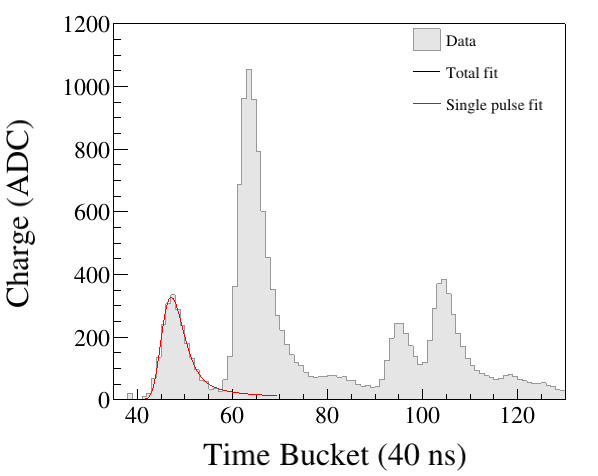
\includegraphics[width=.4\textwidth,valign=t]{psa0.png} \label{fig:psa0}}}%
    \qquad
    \subfloat[$\mathrm{2^{nd}}$ iteration]{{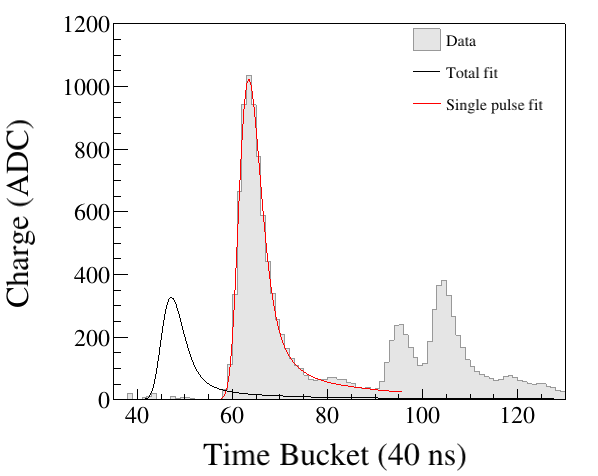
\includegraphics[width=.24\textwidth,valign=c]{psa1.png} \label{fig:psa1}}}%
    \subfloat[$\mathrm{3^{nd}}$ iteration]{{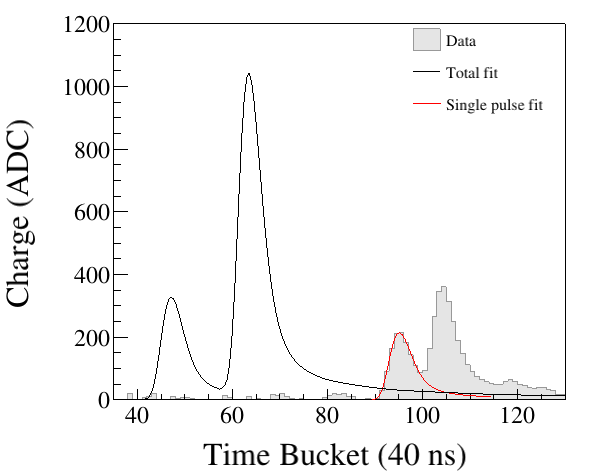
\includegraphics[width=.24\textwidth,valign=c]{psa2.png} \label{fig:psa2}}}%
    \subfloat[$\mathrm{4^{nd}}$ iteration]{{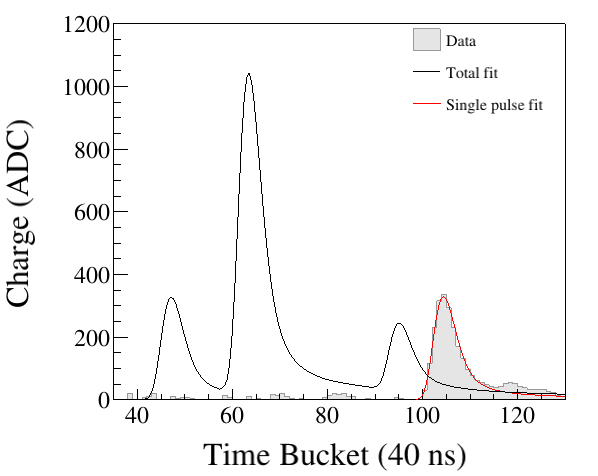
\includegraphics[width=.24\textwidth,valign=c]{psa3.png} \label{fig:psa3}}}%
    \subfloat[Final output of the PSA]{{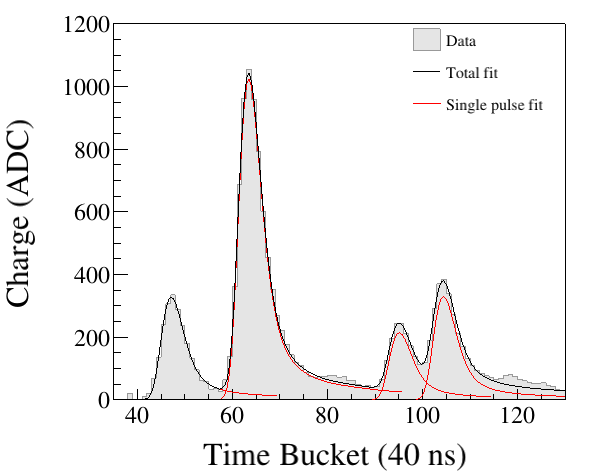
\includegraphics[width=.24\textwidth,valign=c]{psa4.png} \label{fig:psa}}}%

  	\caption{Example of the pulse shape algorithm through each step in processing a given pad. }
	\label{fig:psaTask}
\end{figure}


\subsection{Helix Tracking}
%Cluster cut
%ellipsoid cut
\label{sec:helixtrack}

 The function of the  helix track finding algorithm is to sort the hit cloud into unique sets of hits representing tracks. This is performed by a Riemann track finding algorithm where the Cartesian space is mapped onto a Riemann sphere. This is a particular transformation in which unique helices in the Cartesian space form great circles on the Riemann sphere. This is particularly useful since hits which correspond to a track form a helix in the Cartesian space of the TPC coordinates. It is difficult to search for tracks in the hit cloud by fitting a general helix to different combinations of hits. It is much easier to search for collection of hits by fitting a plane to the great circles which are formed on the Riemann sphere. More details on the Riemann tracking can be found here \cite{spiritroot_paper}. From here the set of hits which form a unique track are stored into a new helix track container called the STHelixTrack class. 
 

%\paragraph{Definition of clustering}
The hits within a helix track are dense and the position resolution of an individual hit is not very precise. As discussed in Section~\ref{sec:prf}, the TPC achieves sub-millimeter position resolution by combining neighboring pads into clusters using the Pad Response Function (PRF). In the helix track finding task, the hits are further reduced into more precise clusters. A brief description of the method of clustering is illustrated in Figure \ref{fig:topview}. We have found that it is sufficient to simply cluster hits along one direction, either along the x or z-direction, depending on which direction is most perpendicular to the track. For example, the three clusters at the bottom of Figure \ref{fig:topview} are clustered along the x-axis, and the upper three are along the z-axis. The bold pads highlight the hits belonging to an example cluster from each set. Since we decide to cluster only in one direction, there is a natural inflection point in a track where the direction of clustering must switch. This switching point is determined by the crossing angle of the track $\theta$, which is defined as the angle between the tangent of the track, projected onto the pad plane, and the x-axis -- at a particular cluster location. In this definition, $\theta = \ang{90}$ corresponds to the case when the track is going along the z-axis and $\theta = \ang{0}$ for a track going along the x-axis.  The clustering direction in the case $\ang{45} < \theta \leq \ang{90} $ is along the x-direction. For tracks with angles $\ang{0} < \theta \leq \ang{45}$ we cluster along the z-axis. 

 

\begin{figure}[!htb]
\centering
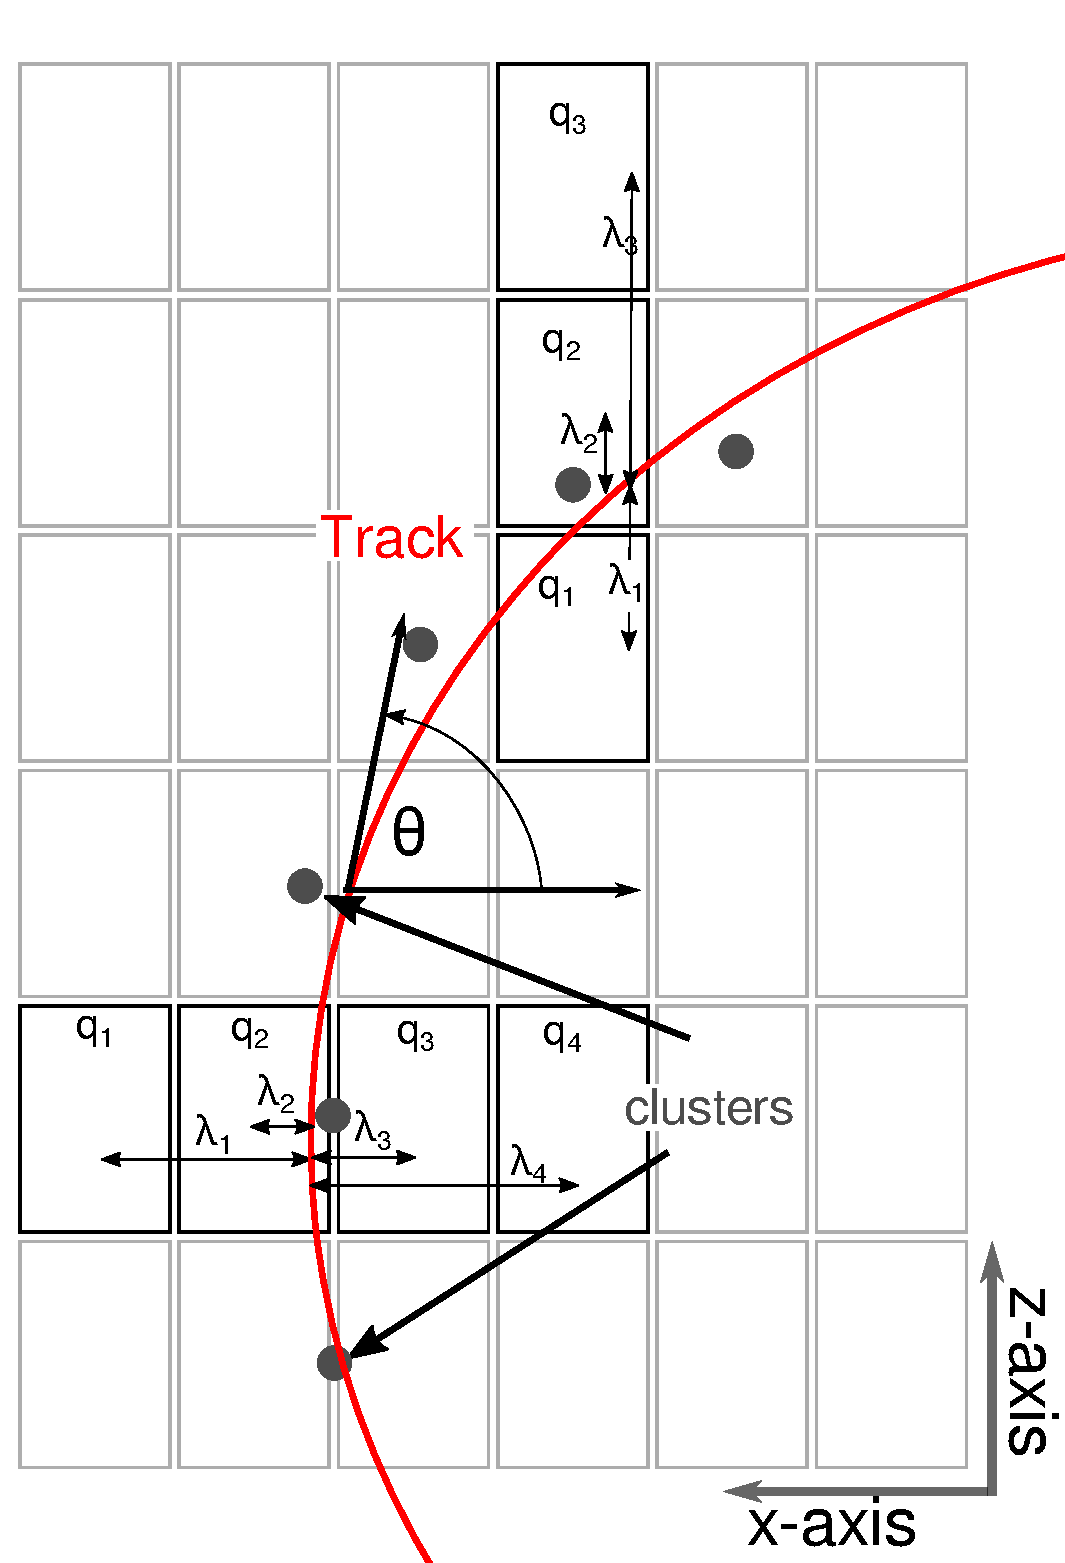
\includegraphics[scale=.5]{top_view_helix_ext.pdf}
\caption{Top down view of a fit to a track passing through several pads. Here we outline the pads in bold, where the charges $q_i$ represent the charged deposited on each pad. In this example, three clusters at the bottom are clustered in the x-direction and for the upper three clustered in the z-direction. The cluster for each group of hits represents the average position of the track. The track fit represents the position of the avalanche, $\bar{x}$,  where the position from the center to each pad to the $\bar{x}$ position is defined as $\lambda_i$.}
\label{fig:topview}
\end{figure}

 The position along the clustering direction, $\overline{X}$, is calculated as the charge-weighted average, $\overline{X} = \sum_i q_ix_i$, where $q_i$ and $x_i$ are the charge and position of the i-th hit in the cluster. The other direction is set to the center of the pad. For example, if we are clustering hits along the x-axis, the z-position is set to the center of the pad in the z-direction and vice versa. Switching the clustering direction gives better position resolution than if we clustered only along one direction. You can imagine if we calculated the clusters only along the x-axis, tracks with $\theta \approx 0^{\circ}$ the x-position is not well defined. The cluster position and charge are stored into a new container representing the cluster called the STHitCluster class. All the clusters which belong to a particular helix track is also stored in the corresponding STHelixTrack class. 

\subsection{Correction Task}
\label{sec:corrTask}
%extend dynamic range
%PRF cut
%space charge correciton
In this task the hit distribution, within a given cluster, is checked against the measured PRF discussed in Section~\ref{sec:prf}. Figure~\ref{fig:prfpimData} shows black lines around the measured PRF in the data representing gates defining the acceptable PRF region. If the charge distribution of the hits in a particular cluster is such that less than 50\% of the hits lie within this PRF gate, the cluster is thrown out from the track. Later, in Section~\ref{sec:expPRF}, we will describe how to define the PRF for a cluster. Clusters which do not follow this PRF gate usually have been corrupted in some way. Typically this occurs when charges from other nearby tracks mix, distorting the hit distribution which corrupts the energy loss and position of the cluster. This tends to occur most frequently in the dense region surrounding the target, where the track density is high. But it may occur along the track for any other reason. The width of the gate is to allow for a reasonable range of PRF values to be accepted, without biasing the data too much.   

%CONSIDER SHOWING SOME PROOF OF IT IN ACTION 

This correction task also handles several other important corrections. The first is a novel algorithm which extends the dynamic range of the electronics and is discussed in detail in Section~\ref{sec:extendDynamicRange}. The other correction task that is handled here is the space charge correction which will be discussed in more detail in Section~\ref{sec:spacecharge}. These two corrections represent the most significant corrections that greatly improve the data. 

\subsection{Momentum and track reconstruction (GENFIT)}
After all of the corrections are applied to the clusters, the cluster's position and charge values are then passed to a software package which reconstructs the momentum of the track called GENFIT. GENFIT utilizes a Kalman fitting algorithm which returns the estimated momentum and charge values for a given track \cite{genfit}. These values are then stored into a new track container called the STRecoTrack class. 

This task is repeated a second time, but this time including the vertex as a constraining point in which all tracks are refitted. In this way, the momentum resolution is greatly improved by adding the vertex as a constraining point; since the BDC detectors, described in Section~\ref{sec:bdc}, provide very accurate x and y values for the vertex location on the target. The energy loss of the track is calculated by the truncated mean method described in Eq.~\ref{eq:truncmean}. The GENFIT task represents the final part of the analysis pertaining to track reconstruction. From here the PID can be constructed using the energy loss, momentum, and charge information. 

\subsection{Vertex tracking (RAVE)}
\label{sec:vertex}
After all tracks are reconstructed by GENFIT, the tracks are then passed to the RAVE software package which reconstructs the event vertex from a collection of tracks \cite{rave}.  The RAVE vertex is typically referred to as the TPC vertex in this dissertation. It is used primarily to find if an event is on target as will be discussed in Section~\ref{sec:vertexcut}. Off target events stemming from reactions in the active collimator or with the counter gas are rejected this way. After such off-target events are rejected,  we use the BDC vertex and refit the tracks as mentioned in the above section; this leads to more accurate momentum values than the TPC generated vertex provided by the RAVE routine. 



\section{Calibrations and Corrections}
In the following subsections we will discuss in detail the calibrations and corrections happening within the software framework that was outlined above.  

\subsection{Gating grid noise subtraction}
\label{sec:ggnoisesub}
Opening the gating grid is essentially done by shorting the adjacent wires in the gating grid together, and allowing them to reach equilibrium as fast as possible. Due to coupling between the gating grid, the ground plane, and other effects, the impedance of the supply cables was not perfectly matched, causing an imbalance in the current where one side discharged faster than the other side. This caused an under-damped oscillating current in the grid, which created an oscillating residual noise early in the time bucket spectrum. Figure~\ref{fig:ggNoiseSub} shows in the upper panel shows the ADC time bucket spectrum after averaging over 2000 events in a given pad. 
 %The ground grid shielded some of the noise, but the path to ground was on two ends and was not sufficiency for this frequency.
 
\begin{figure}[!htb]
\centering
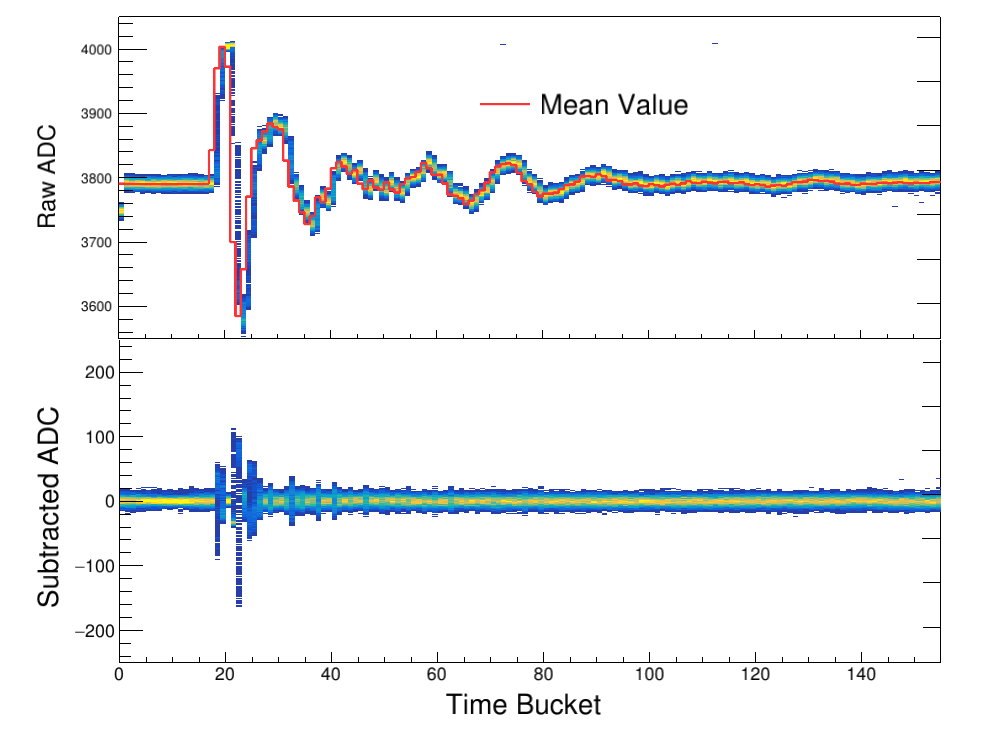
\includegraphics[width=\textwidth]{ggNoise.png}
\caption{Gating grid noise profile and subtraction for a particular pad.}
\label{fig:ggNoiseSub}
\end{figure}

The gating grid noise profile was measured by recording experimental data, only turning off the anode wires. In doing so there are no signals originating from tracks in the TPC and there is only the gating grid noise, since the grid is still being triggered. The gating grid noise was stable for a given pad and the average value --shown as the red line-- can be calculated after averaging over several thousands of events and then removed by subtracting the profile from the real data for each pad.

The bottom panel of Fig.~\ref{fig:ggNoiseSub} shows the gating grid noise self correcting itself, representing a best case scenario. The pedestal -- or base line ADC-- is around 3800 ADC in the upper panel, is automatically subtracted when subtracting the gating grid noise profile since the subtracted ADC spectra is centered around 0. Still, some residual gating grid noise remains even after the subtraction, but it is significantly reduced and its extent is over a much smaller time bucket region. This failure happens in regions where the derivative of the gating grid noise is large. In these areas the ADC value is dependent upon small jitters in the timing of the signal and as a result can vary significantly from event to event. To remove this residual noise in the subtracted spectra we ignored the first 30 time buckets of the readout.

In the experiment the gating grid itself was quite stable in the  ${}^{132}$Sn and ${}^{124}$Sn systems and was not stable in the ${}^{108}$Sn and ${}^{112}$Sn beams, where gating grid resistors broke in these earlier runs many times. Because of this, the gating grid noise was monitored regularly and we took gating grid noise profiles frequently, especially after a gating grid board was replaced. 


%The average noise profile was constructed by averaging all the events in the gating grid runs, pad-by-pad; each pad had a slightly different noise profile since the impedance to each pad was slightly different. It is worth noting that the small electronics noise would be effectively canceled out by averaging over thousands of events. During the first stages of the software, the gating grid noise profile closest to that run would be subtracted from the raw data canceling the gating grid noise in that run. 

\subsection{Cocktail calibration}
\label{sec:cocktail}

\begin{table*}\centering
\ra{1.3}
\begin{tabular}{@{}rrrrrrr@{}}\toprule
& \multicolumn{3}{c}{$100 MeV Target$}\\
\cmidrule{2-4}
Particle &\phantom{abc} & Measured & Corrected & \% Difference Raw & \% Difference Corrected\\
\midrule
p   & 882.8 & 929.5 & 877.3   &  3.7  & -1.0  \\
d   & 817.1 & 831.15 & 797.94 &  1.7  & -2.3\\
\bottomrule
\end{tabular}
\caption{Summary of expected cocktail for the calibration run taken with the Aluminum target. }
\label{tb:cocktail100tar}
\end{table*}

\begin{table*}\centering
\ra{1.3}
\begin{tabular}{@{}rrrrrrr@{}}\toprule
& \multicolumn{3}{c}{$100 MeV$}\\
\cmidrule{2-4}
Particle & Expected & Measured & Corrected & \% Difference Raw & \% Difference Corrected\\
\midrule
p   & 882.8 & 903.5 & 889.0 &  2.0   & -1.6  \\
d   & 817.1 & 898.5 & 874.5 &  2.1   & -2.7\\
\bottomrule
\end{tabular}
\caption{Summary of expected cocktail from the lower beam energy.}
\label{tb:cocktail100}
\end{table*}

\begin{table*}\centering
\ra{1.3}
\begin{tabular}{@{}rrrrrrr@{}}\toprule
& \multicolumn{3}{c}{$300 MeV$}\\
\cmidrule{2-4}
Particle & Expected & Measured & Corrected & \% Difference Raw & \% Difference Corrected\\
\midrule
d   & 1621 & 1704 & 1612   &  5.1 & -0.6  \\
t   & 1612 & 1691 & 1596   &  4.9  & -1.0\\
${}^{4}$He   & 1613 & 1698 &  1595 & 5.3 & -1.1\\

\bottomrule
\end{tabular}
\caption{Summary of expected cocktail from the higher beam energy.}
\label{tb:cocktail300}
\end{table*}

A cocktail of several light charged particles (p,d,t,${}^{3}$He,${}^{4}$He) of well defined magnetic rigidity was produced and measured in the TPC to provide a momentum calibration of the TPC. The magnetic and slit settings of the dipoles in the BigRIPS spectrometer were set so that the momentum resolution of the beam was defined to better than $\delta p/p$ < 1\%. Two magnetic rigidity settings were studied with no target in place. A thick Aluminum target was also inserted to provide a slightly lower energy calibration point for part of the lower rigidity setting, effectively creating three energy calibration points over several particle species. In some cases certain particles were not able to propagate or were strongly attenuated and resulted in measurements of poor statistical precision. 

Since the cocktail beam was a mono-energetic source of particles and rigidity selection in the BigRIPS corresponding to an actual momentum resolution of better than 1\%, we can interpret the  observed momentum resolution as a measurement of the intrinsic TPC momentum for these particles. The momentum resolution in general depends on several factors such as the particle's angle, momentum, charge, track multiplicity, etc. This calibration beam represents an ideal situation where the track was parallel to the pad plane and the track is not affected by the presence of other tracks. The average momentum resolution was measured to be $dp/p = 2\%$ over the full range of particle species for all settings as measured by the sigma of the Gaussian momentum distribution. 

The energy loss resolution can also be directly measured from the monochromatic source provided by the cocktail beam. Each particle species in the cocktail beam has a well defined most probable energy loss;  the energy loss resolution was measured to be approximately 5\% for all particles. These measurements are summarized in Table~\ref{tb:momresolution}.

Since the magnetic dipole setting of the BigRIPS spectrometer is well defined, we can calculate the expected momenta of each particle species measured. The energy losses through various materials in the beam line were propagated using LISE++ software \cite{lise++}. We found that the momenta of light particles in the  cocktail calibration beam differed significantly (up to 5\% ) from the expected values. This is shown in Tables~\cref{tb:cocktail100tar,tb:cocktail100,tb:cocktail300}. We could address this discrepancy by incorporating the smaller horizontal magnetic field components at the edge of the dipole and taking into account the electron drift velocities in the direction of $\vec{E}\times\vec{B}$ as seen from Eq.\ref{eq:elecdrift}. The $\vec{E}\times\vec{B}$ drift velocity causes the electron trajectories to shift toward the +x-axis in the TPC coordinates causing particles of positive charge (going in the -x-axis) to have a higher measured momenta than in reality.  The details of the correction for the $\vec{E}\times\vec{B}$ effect will be discussed later in Section~\ref{sec:spacecharge} in a more general way which also includes the correction for the presence of positive space charge in the field cage volume. The same correction technique was applied here, where the cocktail beam is the special case of zero space charge.

(Tables \ref{tb:cocktail100tar} and \ref{tb:cocktail100}), protons see a slight improvement of about ~1\% whereas the deuterons are over corrected in both settings. In general, all these light particles corrected momentum are of the order of 1\% smaller than value given by the rigidity selection in the BigRIPS separator. This discrepancy could reflect the accuracy of our knowledge of the magnetic field of the SAMURAI dipole. Without a definitive explanation for this discrepancy, we have not attempted further correction of the calculated momenta. We note that it is of the same order as the resolution of the measurement of these momenta.  

\begin{table*}\centering
\ra{1.3}
\begin{tabular}{@{}cc@{}}\toprule
Momentum Resolution \% & <dE/dx> Resolution \% \\
\midrule
1.6  & 4.6\\
\bottomrule
\end{tabular}
\caption{Summary of the estimated momentum and energy loss resolutions.}
\label{tb:momresolution}
\end{table*}

%Apendix of the beam line elements
%apendix of the settings of the bigrips elments
%Picture of cocktail before and after ExB effect
%Table of LISE++ expected cocktail energies ridigity setting of dipole magnets (reference big rips line)


\subsection{Electronics calibration}
\label{sec:elecCalib}

\begin{figure}[!htb]
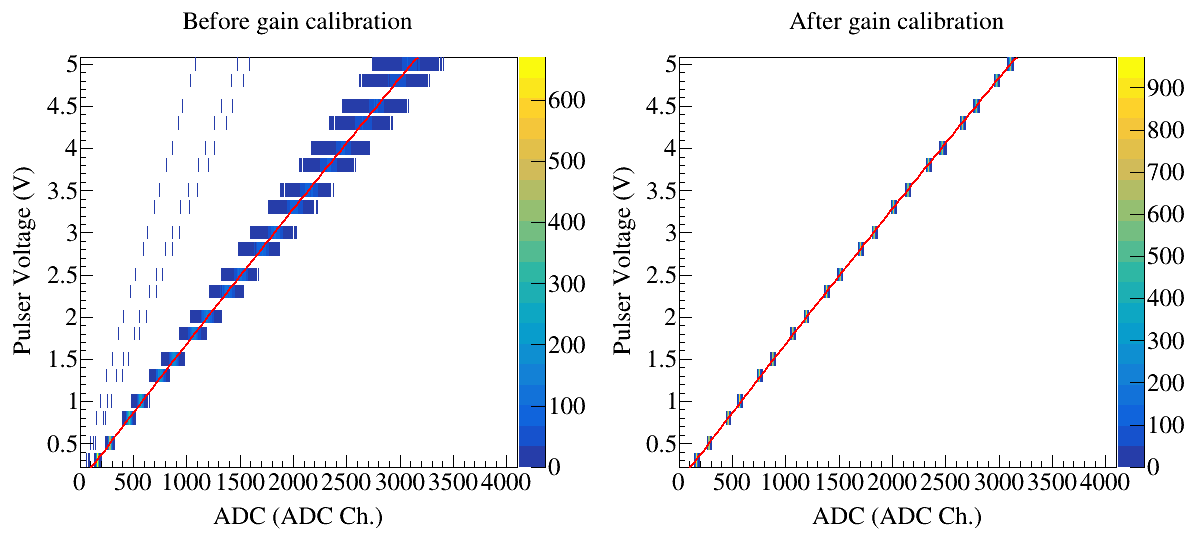
\includegraphics[width=\linewidth]{gaincalib.png}
\caption{Repose of each channel in the electronics to various input voltages of an input signal supplied by a pulse generator.}
\label{fig:gaincalib}
\end{figure}

The electronics were calibrated by measuring the response of each channel to an input signal supplied by a pulse generator. This is a relative calibration technique with the intent to calibrate the varying gains in each channel relative to one another, not an absolute calibration. The pulse was distributed to all the electronics channels by pulsing the ground plane for a range of input voltages. This distributed the pulse evenly across the entire pad plane. The input voltage is plotted as a function of the measured height of the pulse in the electronics channel given in units of ADC in Fig.~\ref{fig:gaincalib}, for every channel. The small variation in each channel can be seen as the wide band around each measurement point. A linear fit is performed to get the calibration line for each channel. A particular channel is chosen which provides a reference calibration to which the slopes of all other channels are calibrated too.   The right panel shows the resulting distribution of channels after calibration, in which the channel variation is reduced significantly. 



\subsection{Anode gain calibration}
\label{sec:anodeCalib}
As discussed in Section~\ref{sec:wireplanes} the voltage of the anode sections 12 and 14 were reduced during the experiment as high currents were observed on the wires due to a leak in the gating grid that has since been corrected \cite{jon}. Out of all the runs used in the analysis in this thesis -- see Appendix~\ref{tb:runList} -- the anode sections 12 and 14 were lowered to \SI{1085}{\volt} for runs 2272-2371 and set to \SI{1214}{\volt} for all other runs. By lowering the voltage on these anode wires, the gas gain is lowered as compared with all the other anode wire plane sections which operate at \SI{1460}{\volt}. To account for the drop in gain, we artificially increase the gain of the pads which lie above these anode wires in the software. The multiplicative factor is estimated by plotting the energy loss in the high gain sections relative to the low gain sections.



\begin{figure}[!htb]
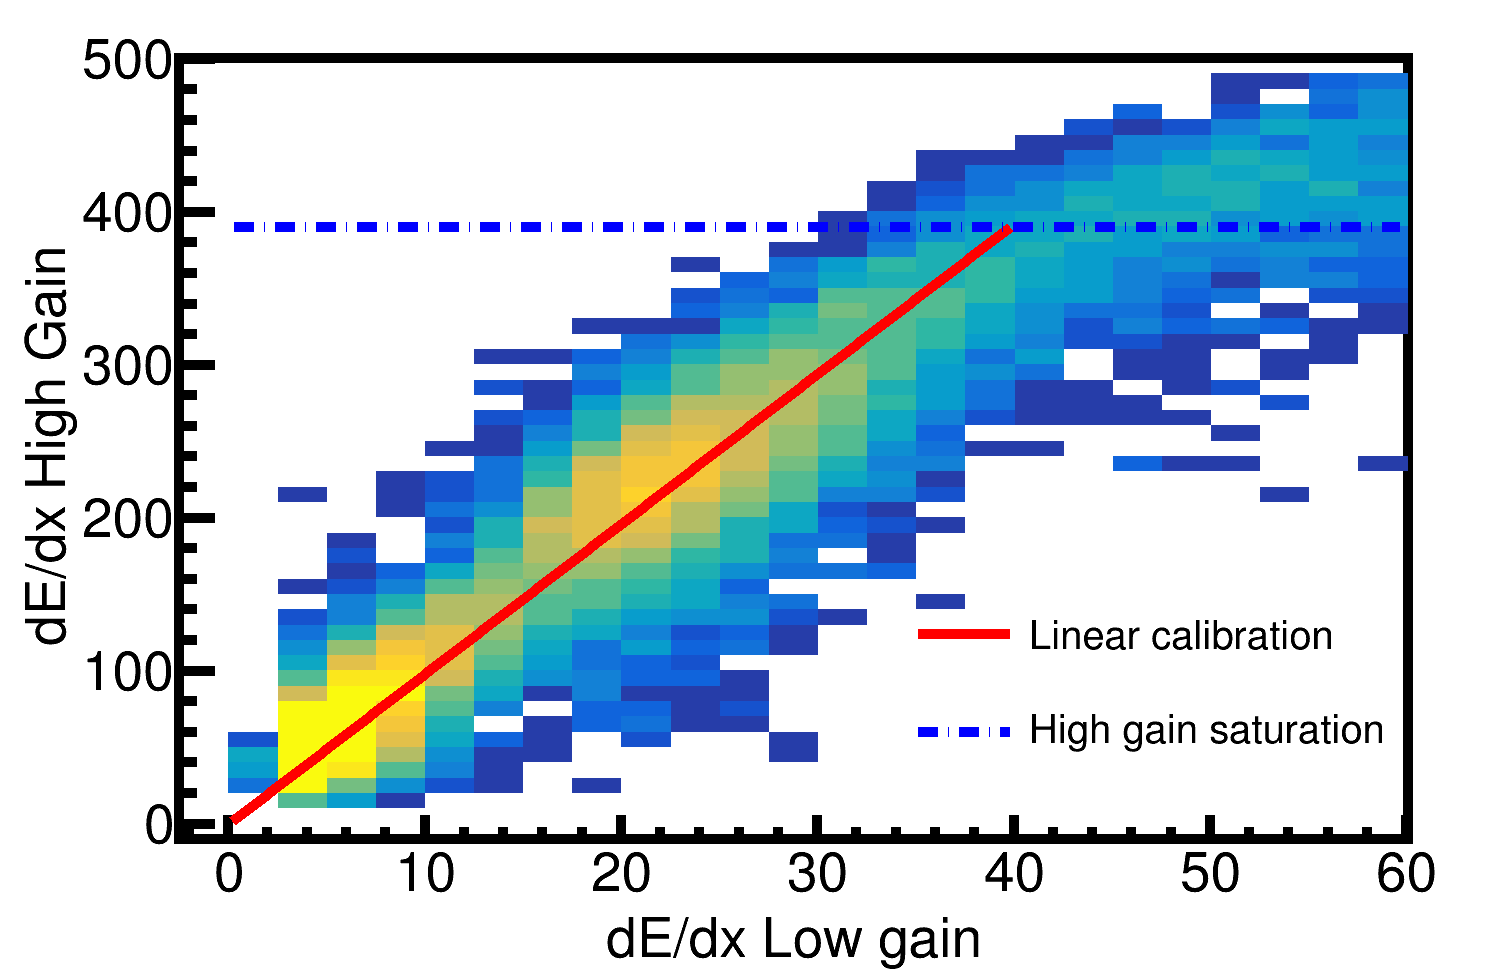
\includegraphics[width=\linewidth]{highlowcal.png}
\caption{Calibration of low and high gain sections of the anode wires.}
\label{fig:highlowcal}
\end{figure}

Figure~\ref{fig:highlowcal} shows the correlation plot of $\langle dE/dx\rangle$ of the high versus the low gain sections. The high gain channel saturates around a value of 400 ADC\si{\per\milli\metre} and plateaus, whereas the low gain does not; this region is left out of the fit. A linear fit was performed for the calibration between the high gain channel $h_c = G\cdot l_c$, where $l_c$ is the value of the low gain channel and $G$ is the gain factor. In the case where the low anode voltage was \SI{1214}{\volt}, the gain factor was $G=9.8$.

%where in the case of \SI{1085}{\volt}, the $G = $.  

 A map defining the gain calibration of each pad is pre-loaded into the software. In the decoder task the raw ADC spectra were multiplied by this gain factor for each channel. The PSA thresholds of those channels also were multiplied by the same gain factor since the noise levels were also artificially magnified as well. 

\subsection{Extending the dynamic range of the Electronics}
\label{sec:extendDynamicRange}

Using a TPC for measurements of HICs in intermediate energy heavy ion collisions presents a different set of challenges as opposed to higher energy experiments. Typically in higher energy experiments fundamental particles are produced with charge $\pm e$. Also, the particles are traveling at higher energies in which the energy losses are near or close to the minimum ionization. In these cases the dynamic range of most TPC electronics can cover a wide range of particles. In nuclear HICs, we are interested in measured particles with charges $Ze$ where Z=1-3, and even higher in some applications. Since the energy loss in the Bethe-Bloch equation, Eq.~\ref{eq:bb}, is proportional to $Z^2$, the range of energy losses reflects the possible range of z values. HIC of intermediate beam energies -- around \SI{300}{\MeVA} -- produce low velocity particles which exist in the $1/\beta^2$ region of Eq.~\ref{eq:bb}, where the energy loss grows dramatically. In this case, the dynamic range of electronics significantly limit the PID as the charge of a particle increases and the velocity decreases, leading to very large and even saturated pulses in the electronics. 

Several TPCs have tried to address this issue by having regions of low and high gain, either in amplification gain or in electronics gain. This mitigates the complete loss of information but introduces a new problem. Particles which deposit large amounts of charge will have good measurements in the low gain areas, whereas particles depositing minimal energy losses will lose information in the same low gain areas. The reconstruction of such tracks will suffer. There are ongoing efforts in the nuclear community to develop new electronics to mitigate these issues by developing more sophisticated  pre-amplifiers and electronics \cite{feanics,feanics2}.  Nevertheless, it is useful to develop a software technique which extends the dynamic range of TPC electronics without the use of new external hardware, which can be particularly useful for experiments which have already taken data with older electronics technologies. In this section we will outline a novel software technique that takes advantage of the PRF described in Section~\ref{sec:prf} and can effectively extend the dynamic range of the TPC electronics. 

The effective dynamic range is very different from the single channel dynamic range depending on how the TPC measurement is used. Typically TPCs are operated inside of a magnetic field for the purpose of reconstructing the momentum of a track, which requires sub-millimeter precision in the position determination along the track path. This is achieved by clustering several pads together as discussed in Section~\ref{sec:helixtrack}. To achieve this at least 2 adjacent pads must be measured, and the precision increases as the number of adjacent pads increases. 

In this case the effective dynamic range is not the single channel dynamic range, but the relative dynamic range between central pad --holding the largest charge-- and the adjacent pads --holding the smaller charges in the PRF distribution. For example, to measure minimum ionizing particles, the Signal-to-Noise-Ratio (SNR) of the pad with the smallest charge in the distribution should be some reasonable value, so that the full charge distribution can be measured. From the PRF in Section~\ref{sec:prf}, we know the central pad in the cluster holds about 80\% of the total charge, whereas the two adjacent pads each hold the remaining 10\%. In the \spirit TPC the electronics gain was set so that the pads have a SNR of 6:1 for minimum ionizing tracks, and therefore the central pad had a SNR of 50:1. The maximum SNR in the central pad -- before the electronics saturate -- the SNR is 800:1. Therefore the maximum SNR is roughly 16 times larger than that of minimum ionizing particles. 

Figure~\ref{fig:intro} shows the theoretical energy loss curves for several particles as a function of rigidity $p/q$. Minimum ionization can be seen to take place around \SI{10}{\kilo\electronvolt\per\centi\metre}. The dashed lines and vertical blue bar in are separated by a factor of 16, representing the effective dynamic range in the \spirit TPC. This dynamic range should be regarded as approximate because the energy loss fluctuates significantly about the most probable energy loss as described in Section~\ref{sec:energyloss}. Nevertheless, the blue dashed lines and vertical blue bar illustrate that the range of energy losses sampled in a fixed gain readout system is limited. One can change the gain and shift the energy loss range that can be sampled, but the dynamic range itself cannot be increased.

  
\begin{figure}[ht!]
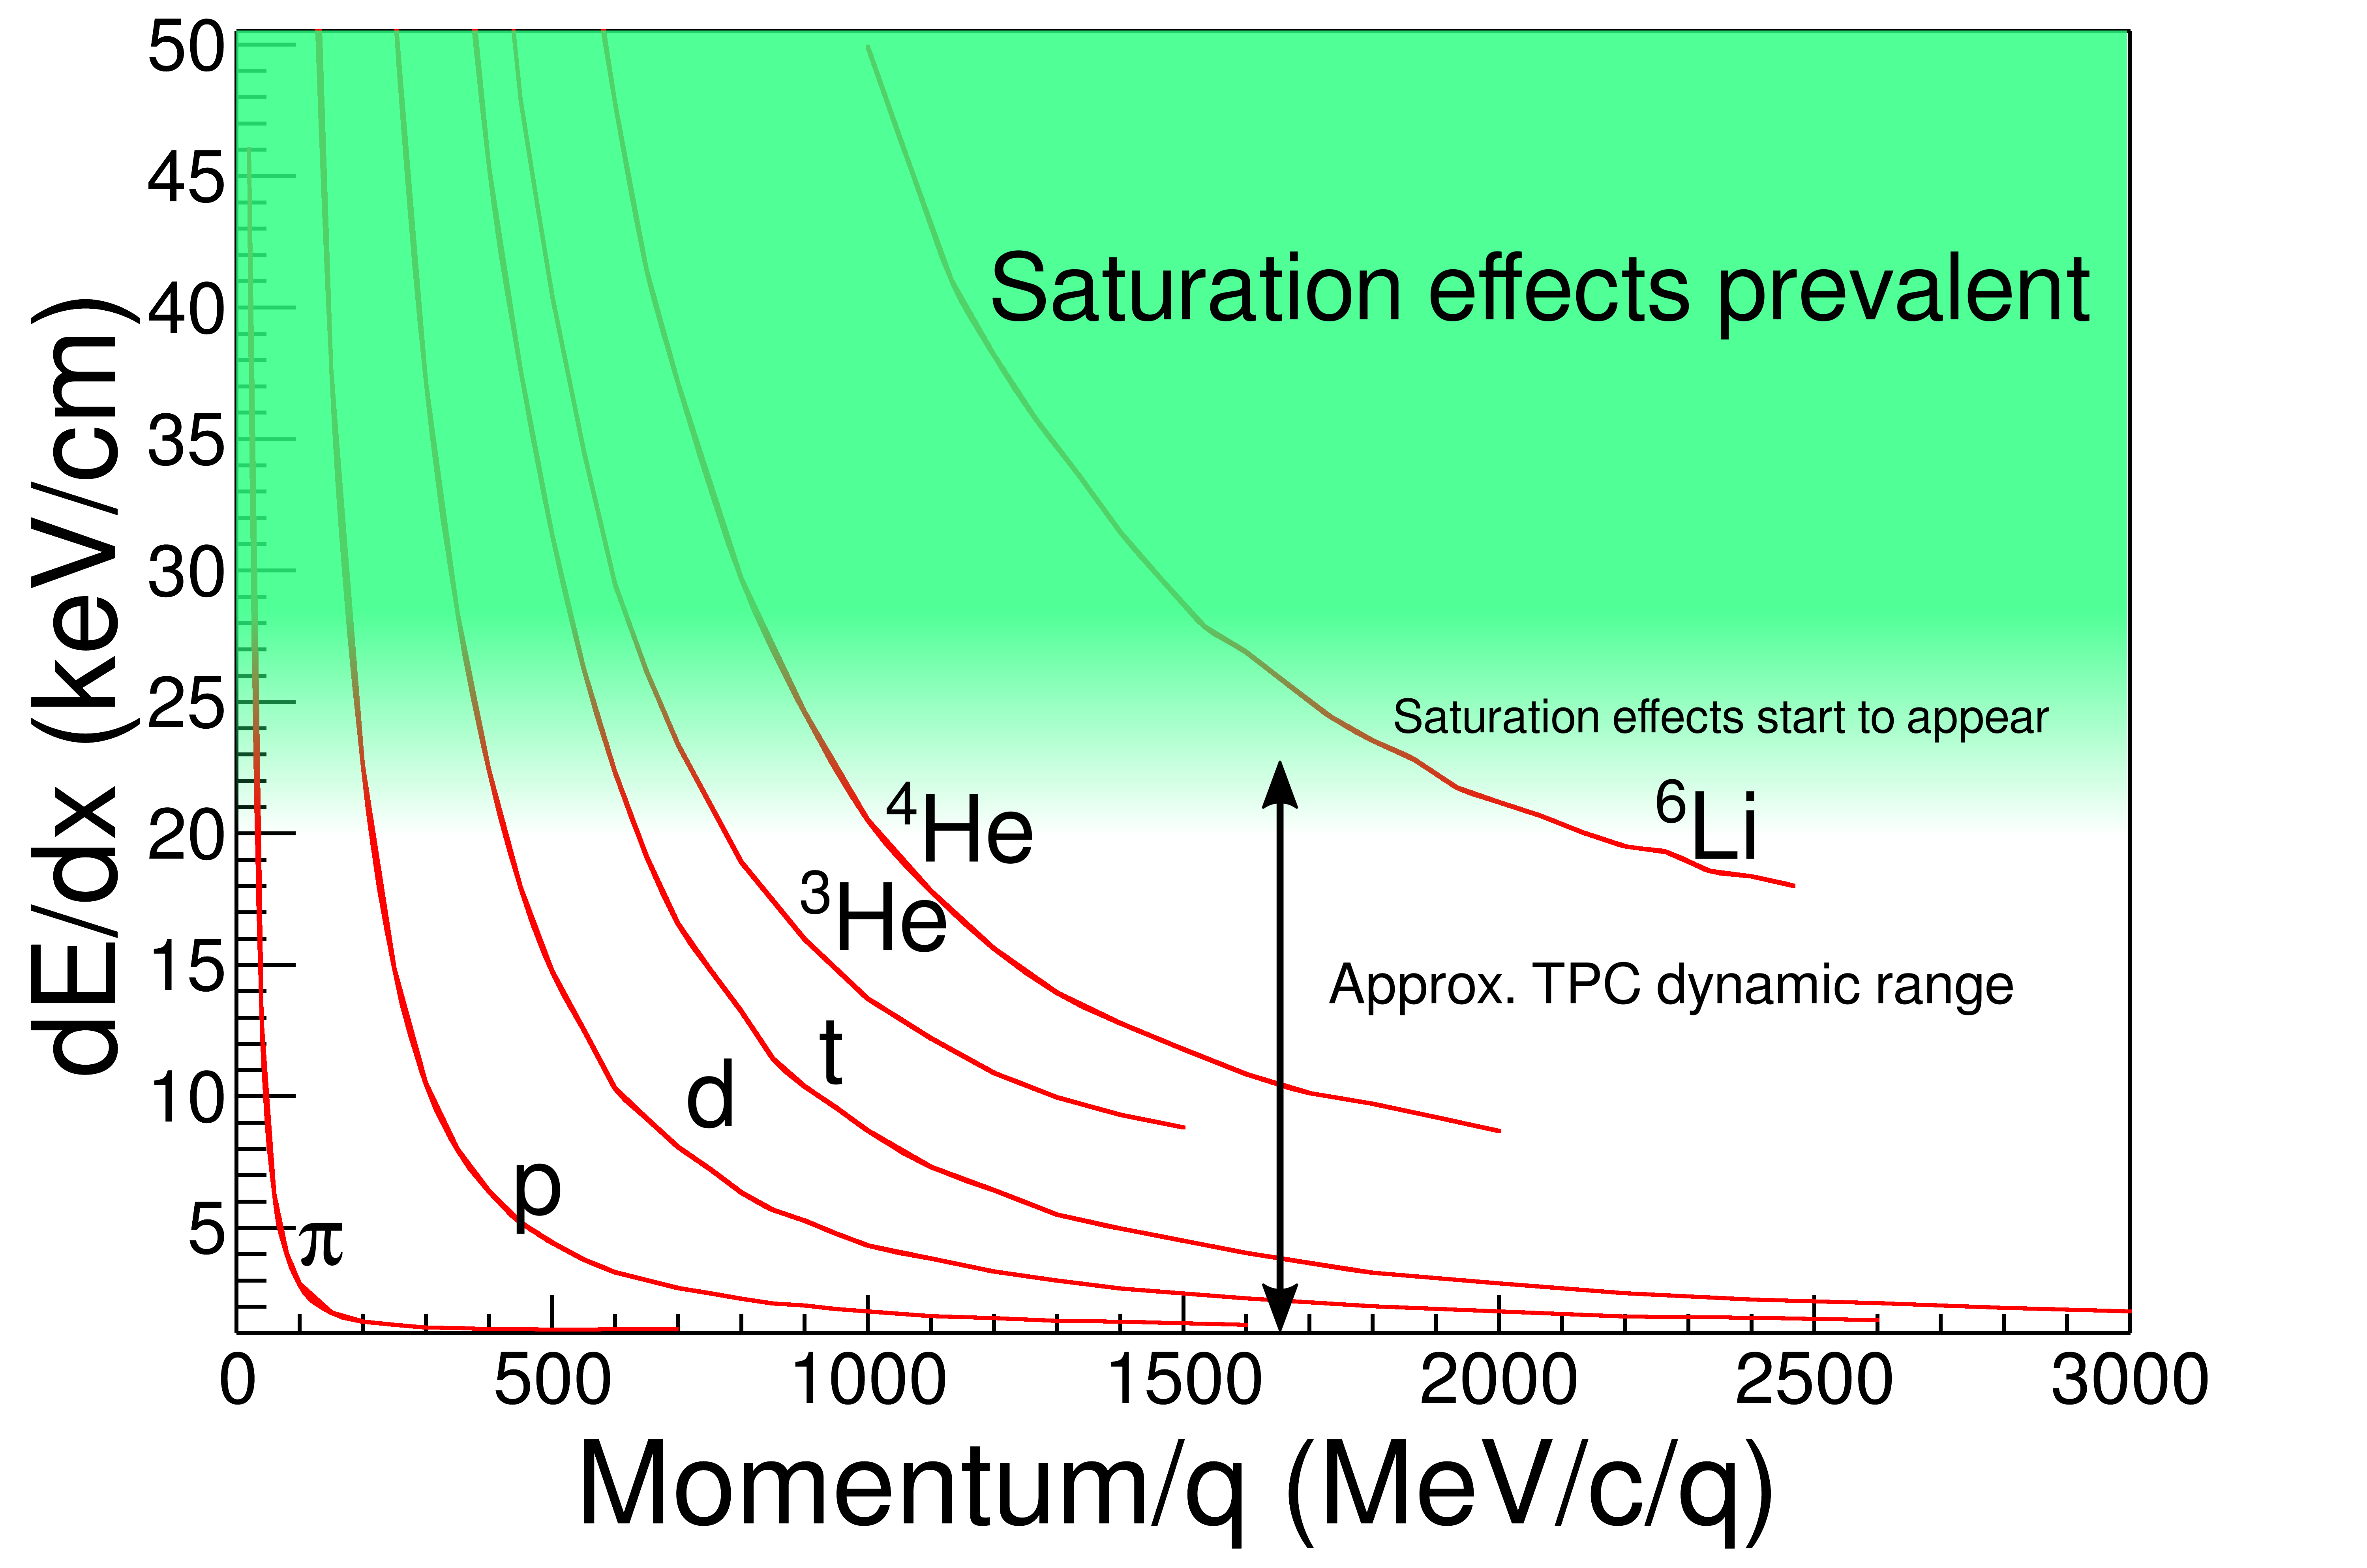
\includegraphics[width=\linewidth]{intrographic}
%\includegraphics[width=\linewidth]{intrographic_2}
\caption{The expected $dE/dx$ lines of different particles are given in red as calculated by Geant4. The approximate dynamic range of the TPC is shown by the vertical bar for the gain setting used in the experiment. Anything outside of this region would be saturated to some degree.}
\label{fig:intro}
\end{figure}


\subsection{Experimental Pad Response Function}
\label{sec:expPRF}
As mentioned in Section~\ref{sec:prf}, the PRF depends on the angle of the track as it crosses the wires and pads. The PRF of the TPC was experimentally determined from non-saturating hits and clusters in tracks at various track crossing angles. As in Fig.~\ref{fig:topview}, we postulate that the PRF is a function of the total charge deposited in a cluster $Q = \sum_i q_i$, and the difference in position of the center of the $i^{th}$ pad, $x_i$, to the mean position $\bar{x} = \sum_i x_i q_i/Q$, defined as,

\begin{equation}
\lambda_i = x_i-\bar{x}. 
\label{eq:lambda}
\end{equation}

The PRF is simply defined as the charge fraction of each pad as a function of $\lambda$, as shown in Equation \ref{eq:prf}. 

\begin{equation}\label{eq:prf}
PRF(\lambda_i) = \frac{q_i(\lambda_i)}{Q}
\end{equation}

Averaging over many events in the experimental data, the resulting PRF is particularly well behaved for the S$\pi$RIT TPC as seen in Fig.~\ref{fig:expprf}. Here we see the deviations from the expected analytic Gatti distribution (black curve). Fitting with a two parameter Gaussian function -- the red curve -- describes the data better. The PRF was fit with a two parameters Gaussian function, where $N_)$ is the normalization coefficient and $\sigma$ the corresponding width:

\begin{equation}\label{eq:gaus}
PRF_{\mathrm{Gaus}}(\lambda) = N_0 e^\frac{-\lambda^2}{2\sigma^2}.
\end{equation}


\begin{figure}[ht!]s
\begin{overpic}[width=\linewidth]{fig5.pdf}
\put(61,55){\contour{white}{ PRF${}_{\mathrm{Gaus}}(\lambda)$ eq. \ref{eq:gaus}  }}
\put(61,49){\contour{white}{ PRF${}_{\mathrm{Gatti}}(\lambda)$ eq. \ref{eq:gatti} }}
\end{overpic}
\caption{Experimental pad response function of many events for a crossing angle of $85^{\circ} < \theta \leq 90^{\circ}$.  }
\label{fig:expprf}
\end{figure}



The shape of the PRF depends on the crossing angle of the track, which determines how wide the charge is distributed along the wire \cite{gatti}. Figure~\ref{fig:prfpimData} shows the PRF for $\pi^-$ tracks versus the crossing angle $\theta$ of the track. The PRF gets wider starting from $90^{\circ}$  until where the clustering switches directions at $\ang{45}$. If we did not switch clustering directions the PRF would become wider until it was a uniform distribution and there was no position resolution. Switching shows the opposite trend where the PRF becomes narrower going from $45^{\circ}$ to $0^{\circ}$, as the position resolution gets better.

\begin{figure}[!htb]
     \centering
	 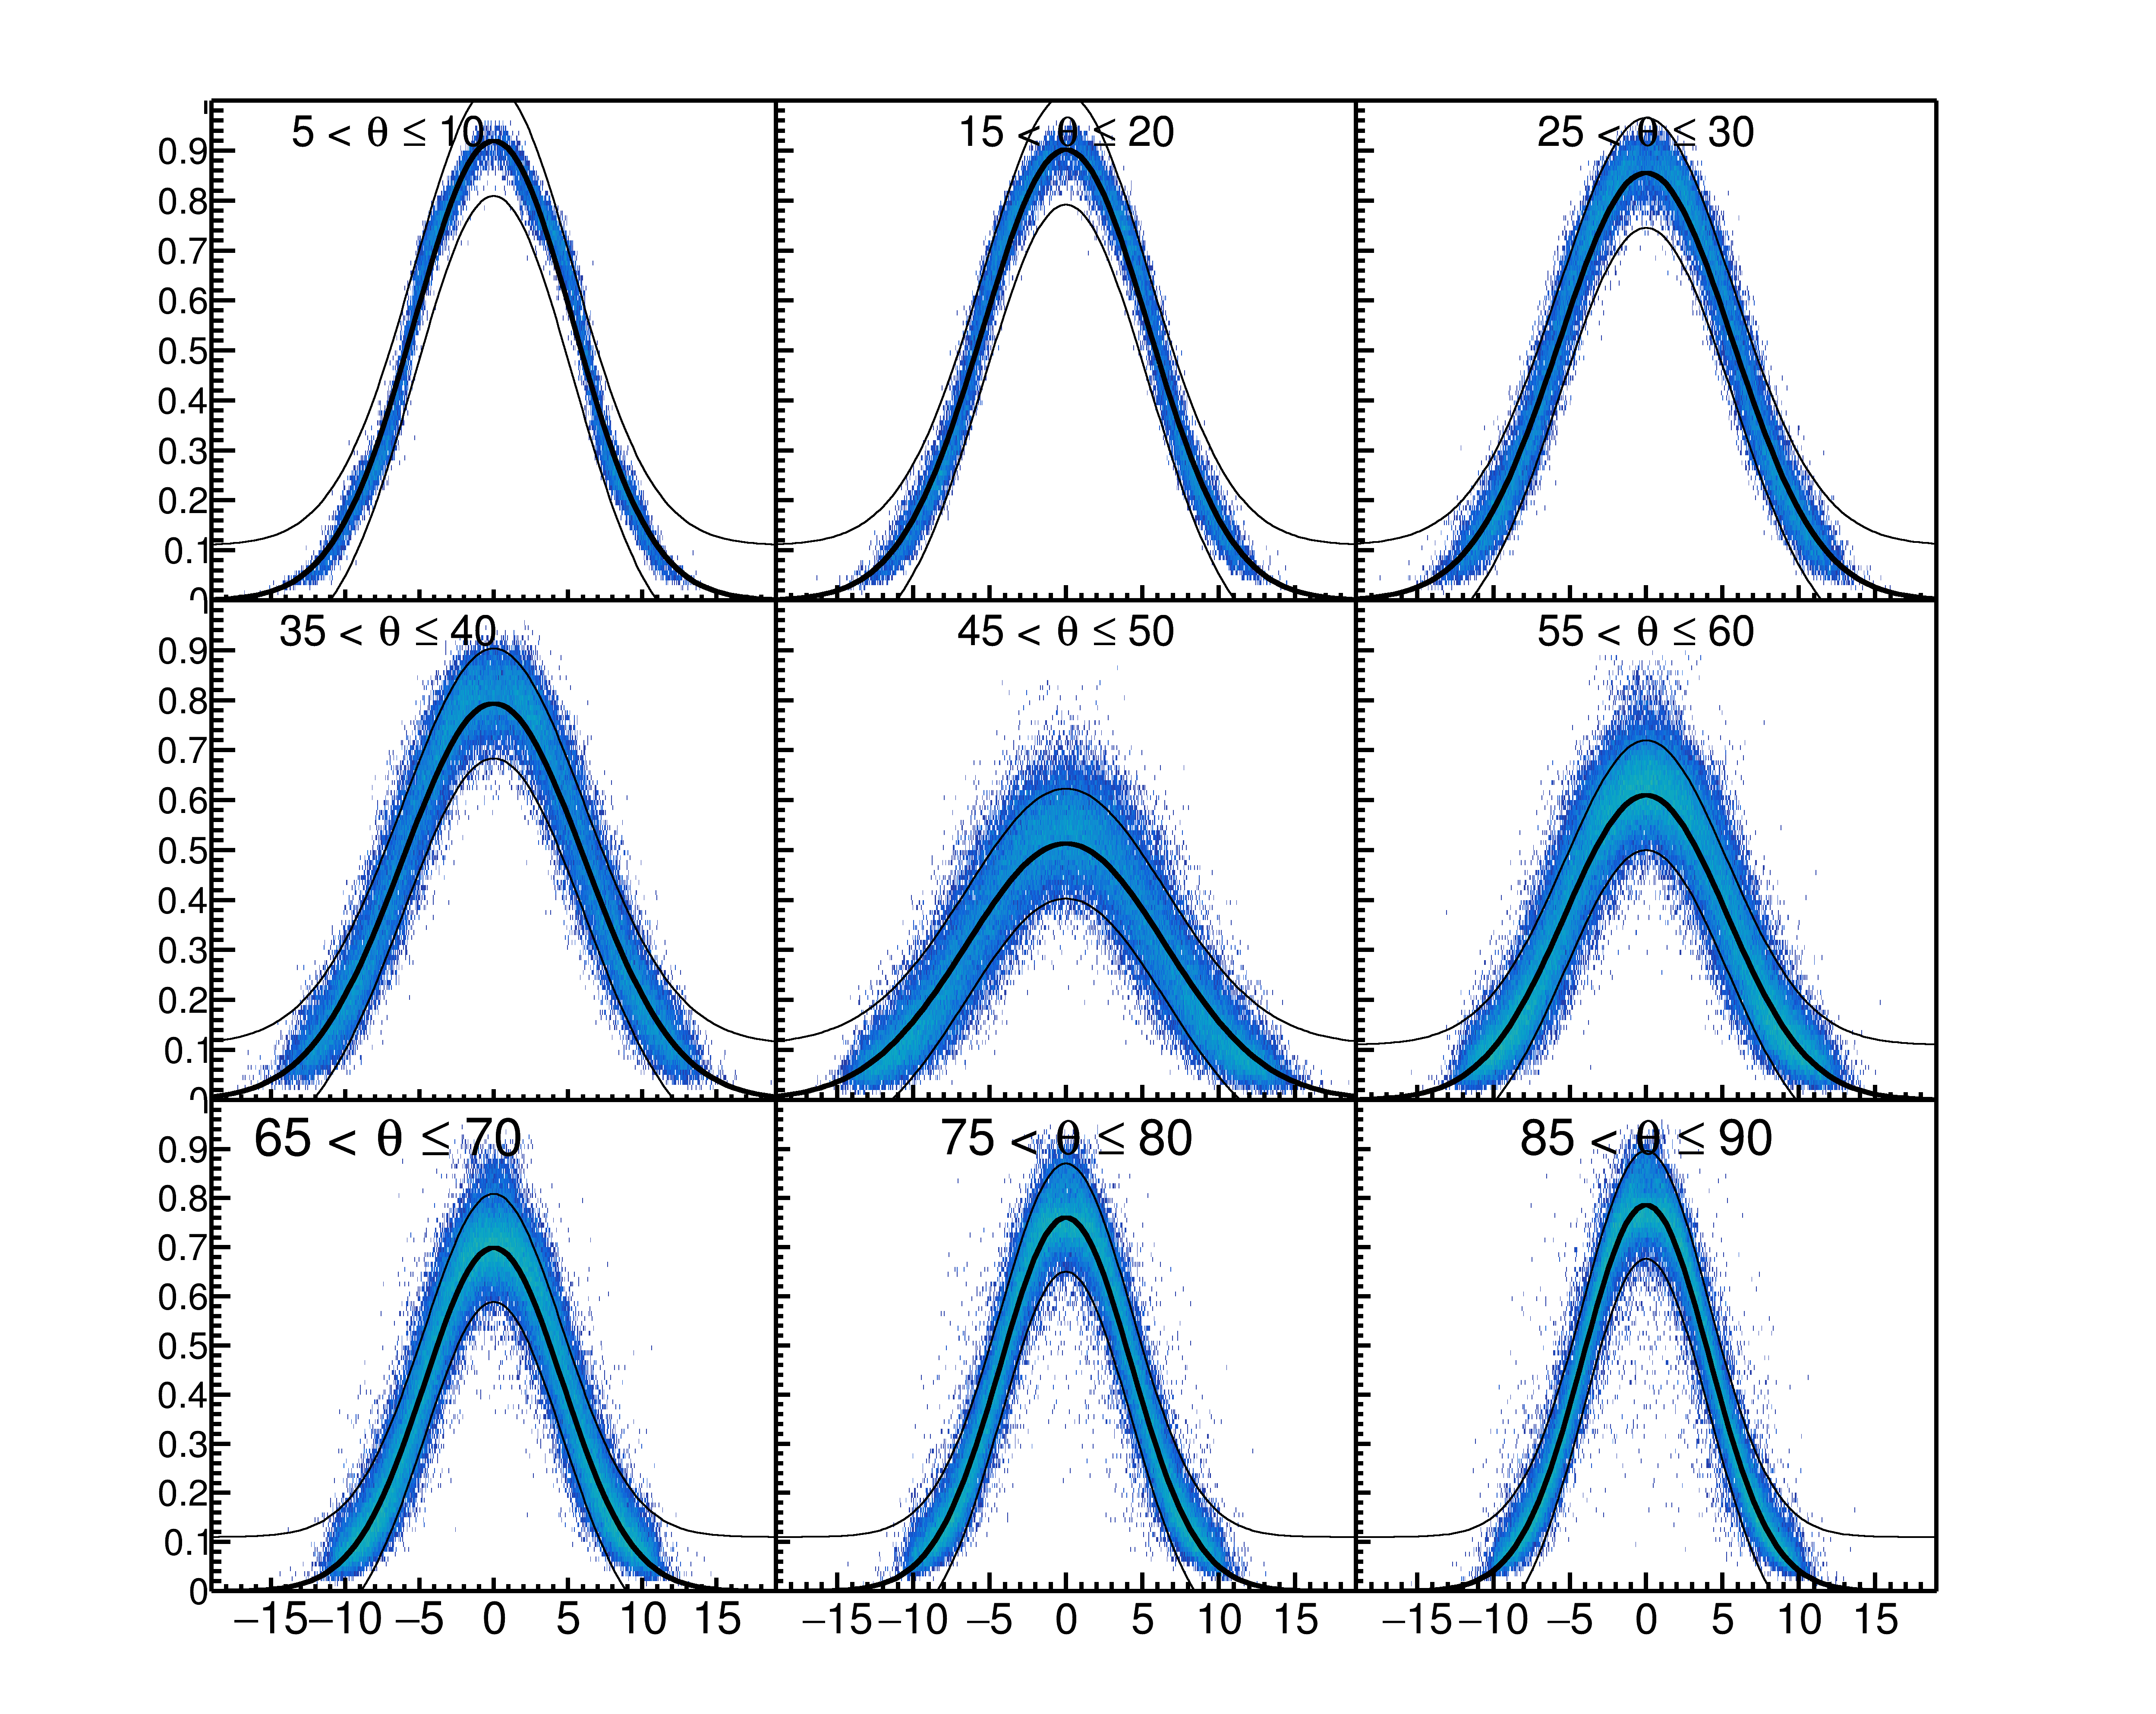
\includegraphics[width=\textwidth]{PRFs_data_wcut.png}
     \caption{Pad Response Function of $\pi^-$ tracks in experimental data. }
     \label{fig:prfpimData}
\end{figure}

\begin{figure}[ht!]
\vspace{5mm}
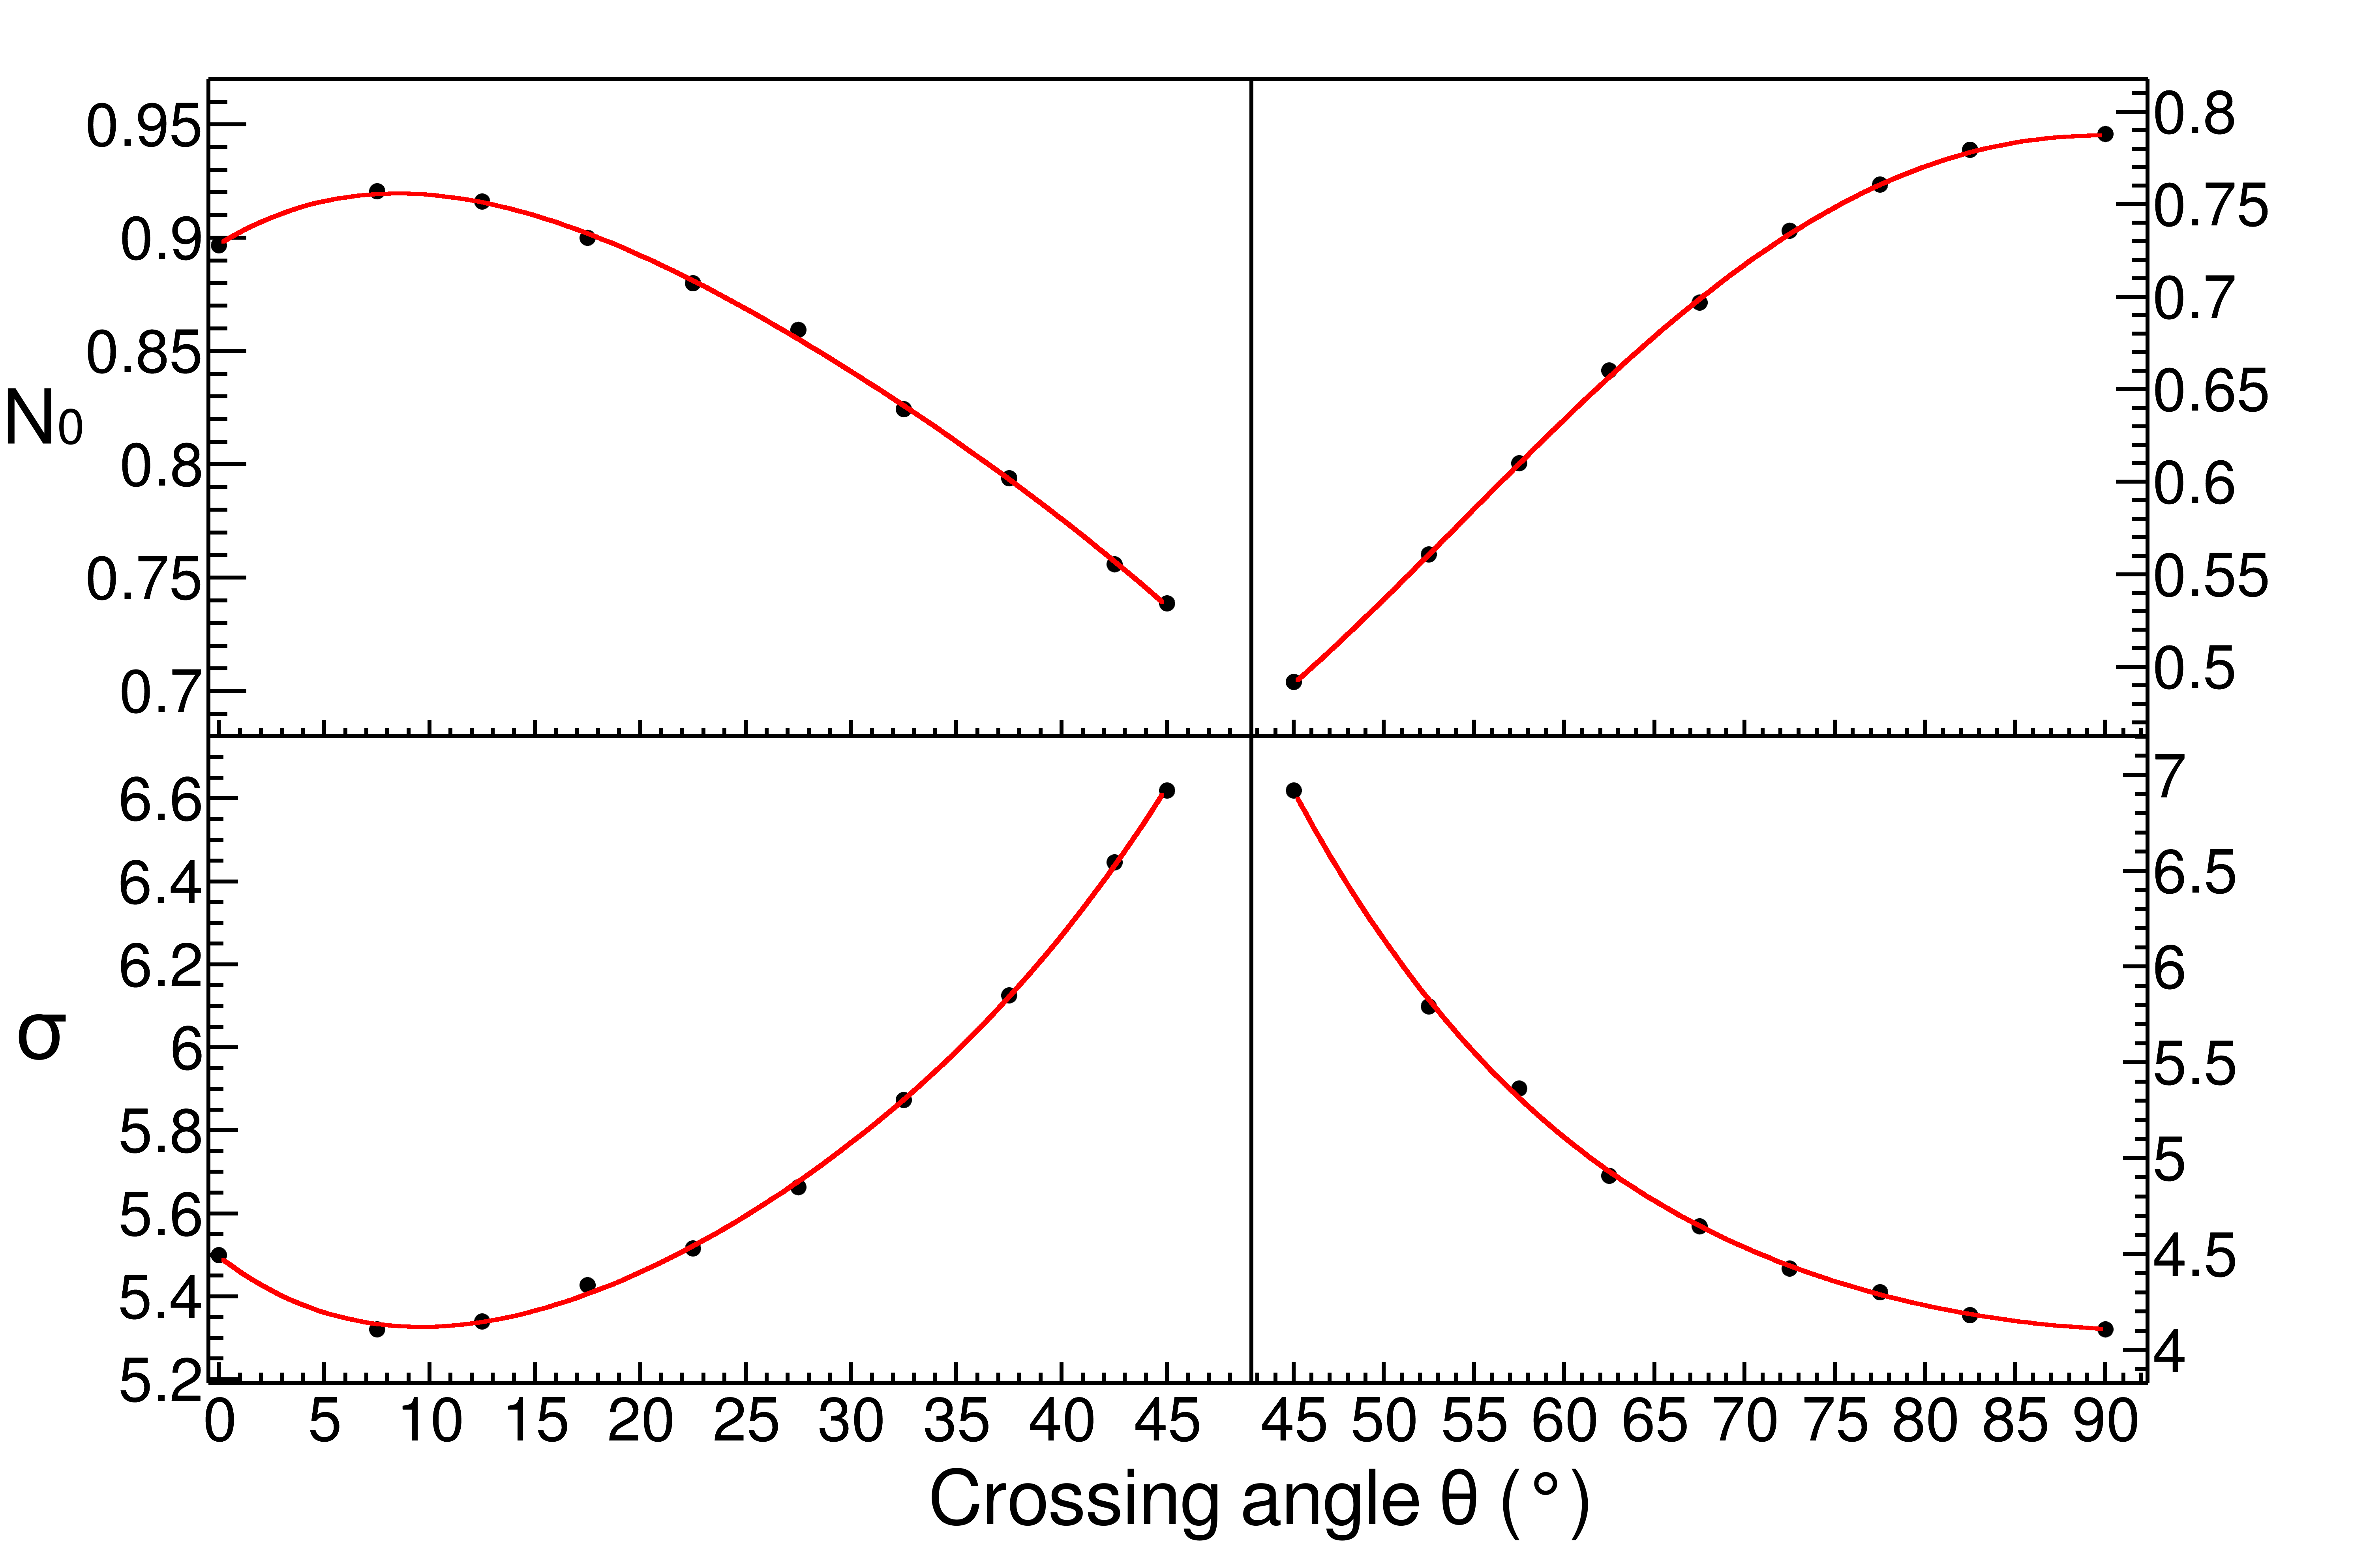
\includegraphics[width=\linewidth]{fig7}
\caption{Parameters $N_{0}$ and $\sigma$ as a function of the crossing angle $\theta$ with the $4^{th}$ order polynomial fits.}
\label{fig:normsigma}
\end{figure}

\begin{comment}
\begin{table}
\centering
 \begin{tabular}{||c c c c c c||} 
 \hline
 Coefficient & $c_0$ & $c_1$ & $c_2$ & $c_3$ & $c_4$ \\ [0.5ex] 
 \hline\hline
 $0 < \theta < 45$ & & & & &  \\ [.25ex]
 \hline
 $N_0$ & .897 & 5.766E-3 & -4.263E-4 & 7.444E-6 & 5.705E-8 \\ 
 \hline
 $\sigma$ & 5.496 & -3.920E-2 & 2.693E-3 & -5.208E-5 & 5.334E-7\\
 \hline
 $45 < \theta < 90$ & & & &  & \\ [.25ex]
 \hline	
 $N_0$ & 1.220 & -6.258E-2 & 1.608E-3 & -1.492E-5  & 4.654E-8 \\
 \hline
 $\sigma$ & 31.368 & -1.109 & 1.779E-2 & -1.336E-4 & 3.940E-7\\
 \hline
\end{tabular}
\caption{Coefficients of the $4_th$ order polynomial fit to the Gaussian parameters $N_0$ and $\sigma$. The polynomial form is given as $c_0 + c_1 x + c_2 x^2 + c_3 x^3 + c_4 x^4$}
\label{tb:coeff}
\end{table}
\end{comment}
 
The Gaussian fit was performed on each PRF for a crossing angle steps of  $\ang{5}$ ranging from $\ang{0} < \theta \leq \ang{90}$. Figure~\ref{fig:normsigma} shows the two parameters resulting from fitting the Gaussian function -- Eq.~\ref{eq:prfgaus} -- which are plotted versus $\theta$. A $4^{th}$ order polynomial fit of these parameters allowed for interpolating for any given $\theta$ value, which is shown as the black line. Once we have this interpolation, we can predict the PRF for any given value of $\theta$. 


\subsection{Method of Desaturation}
\label{sec:desat}

\begin{figure}[ht!]
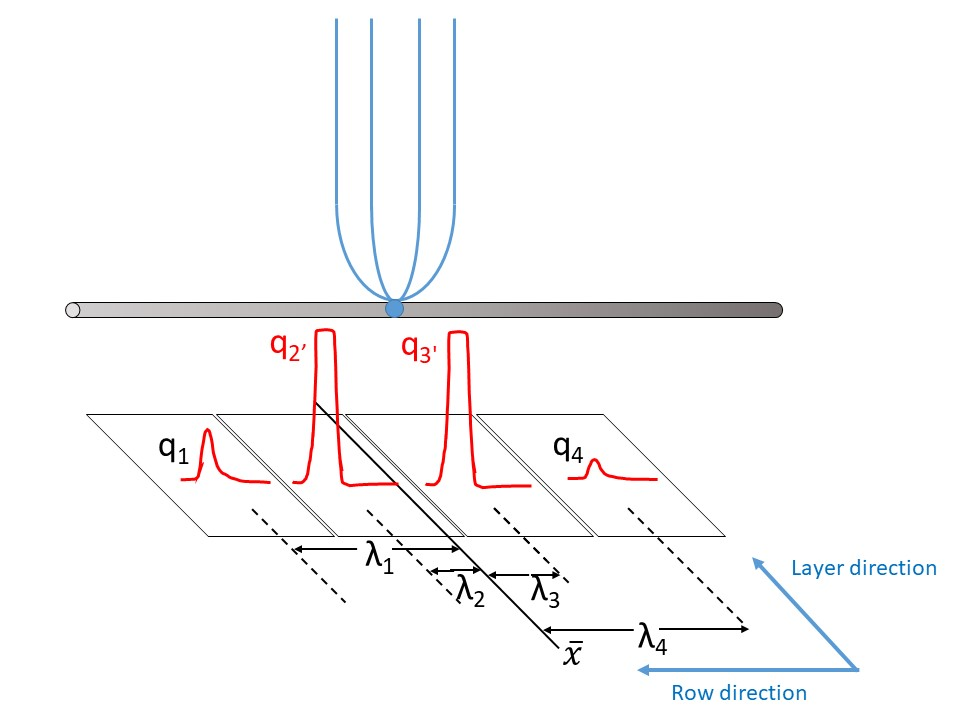
\includegraphics[width=\linewidth]{saturated_pads}
\caption{A typical case of a saturating event. The red pulses represent the time bucket signal for each collected charge. The pads directly underneath the avalanche point, $q_{2'}$ and $q_{3'}$, are saturated while pads farther away, $q_1$ and $q_4$ are not saturated.}
\label{fig:satpad}
\end{figure}

In the following, we will use the term \emph{desaturation} to describe the technique of correcting saturated pads. Figure~\ref{fig:satpad} shows a typical situation of saturated hits in a cluster. When an avalanche causes a large enough induced signal, the pads directly underneath the avalanche collect the largest charge becoming saturated, denoted here as $q_{2\textprime}$ and $q_{3\textprime}$. Pads further away collect less charge and typically are not saturated, detonated here as $q_{1}$ and $q_{4}$. Although the charge values in the saturated channels are lost, we know that the distribution of all charges must follow the PRF; this is fundamental operating principle of all TPCs. We have already measured the PRF as a function of crossing angle in Section~\ref{sec:expPRF}, and from the tracking information, we know the crossing angle of the track at a given cluster and therefore the PRF corresponding to that cluster. 

We assume the distance of each pad to fitted track, $\lambda_i$ , Eq.~\ref{eq:lambda}, is fixed, defining the fraction of charge each pad receives as defined by the $PRF(\lambda_i)$ function. To determine the best estimate for the charge values of each saturated pad, a chi squared function is minimized,

\begin{equation}\label{eq:chi}
\chi^2 = \sum_i \frac{(q_i^{\mathrm{obs}} - q_i^{\mathrm{expect}})^2}{q_i^{\mathrm{expect}}},
\end{equation}


where $q_i^{\mathrm{obs}}$ are the non-saturated charges and $q_i^{\mathrm{expect}}$ are the charge values expected for that pad as calculated from the PRF, $q_i^{\mathrm{expect}} = Q\cdot PRF(\lambda_i)$. The saturated charge values $q_{i}^{\textprime}$ are treated as unknown variables and are allowed to vary in the $\chi^2$ minimization routine, they enter the calculation when they are added to get the total charge $Q = \sum q_i + \sum q_i^{'}$. The minimum $\chi^2$ value returns the best estimate for the unknown saturated charge values. The saturated hit charges are updated to reflect these estimates and the cluster position and charge are updated accordingly.


\begin{figure*}[!htb]
\centering
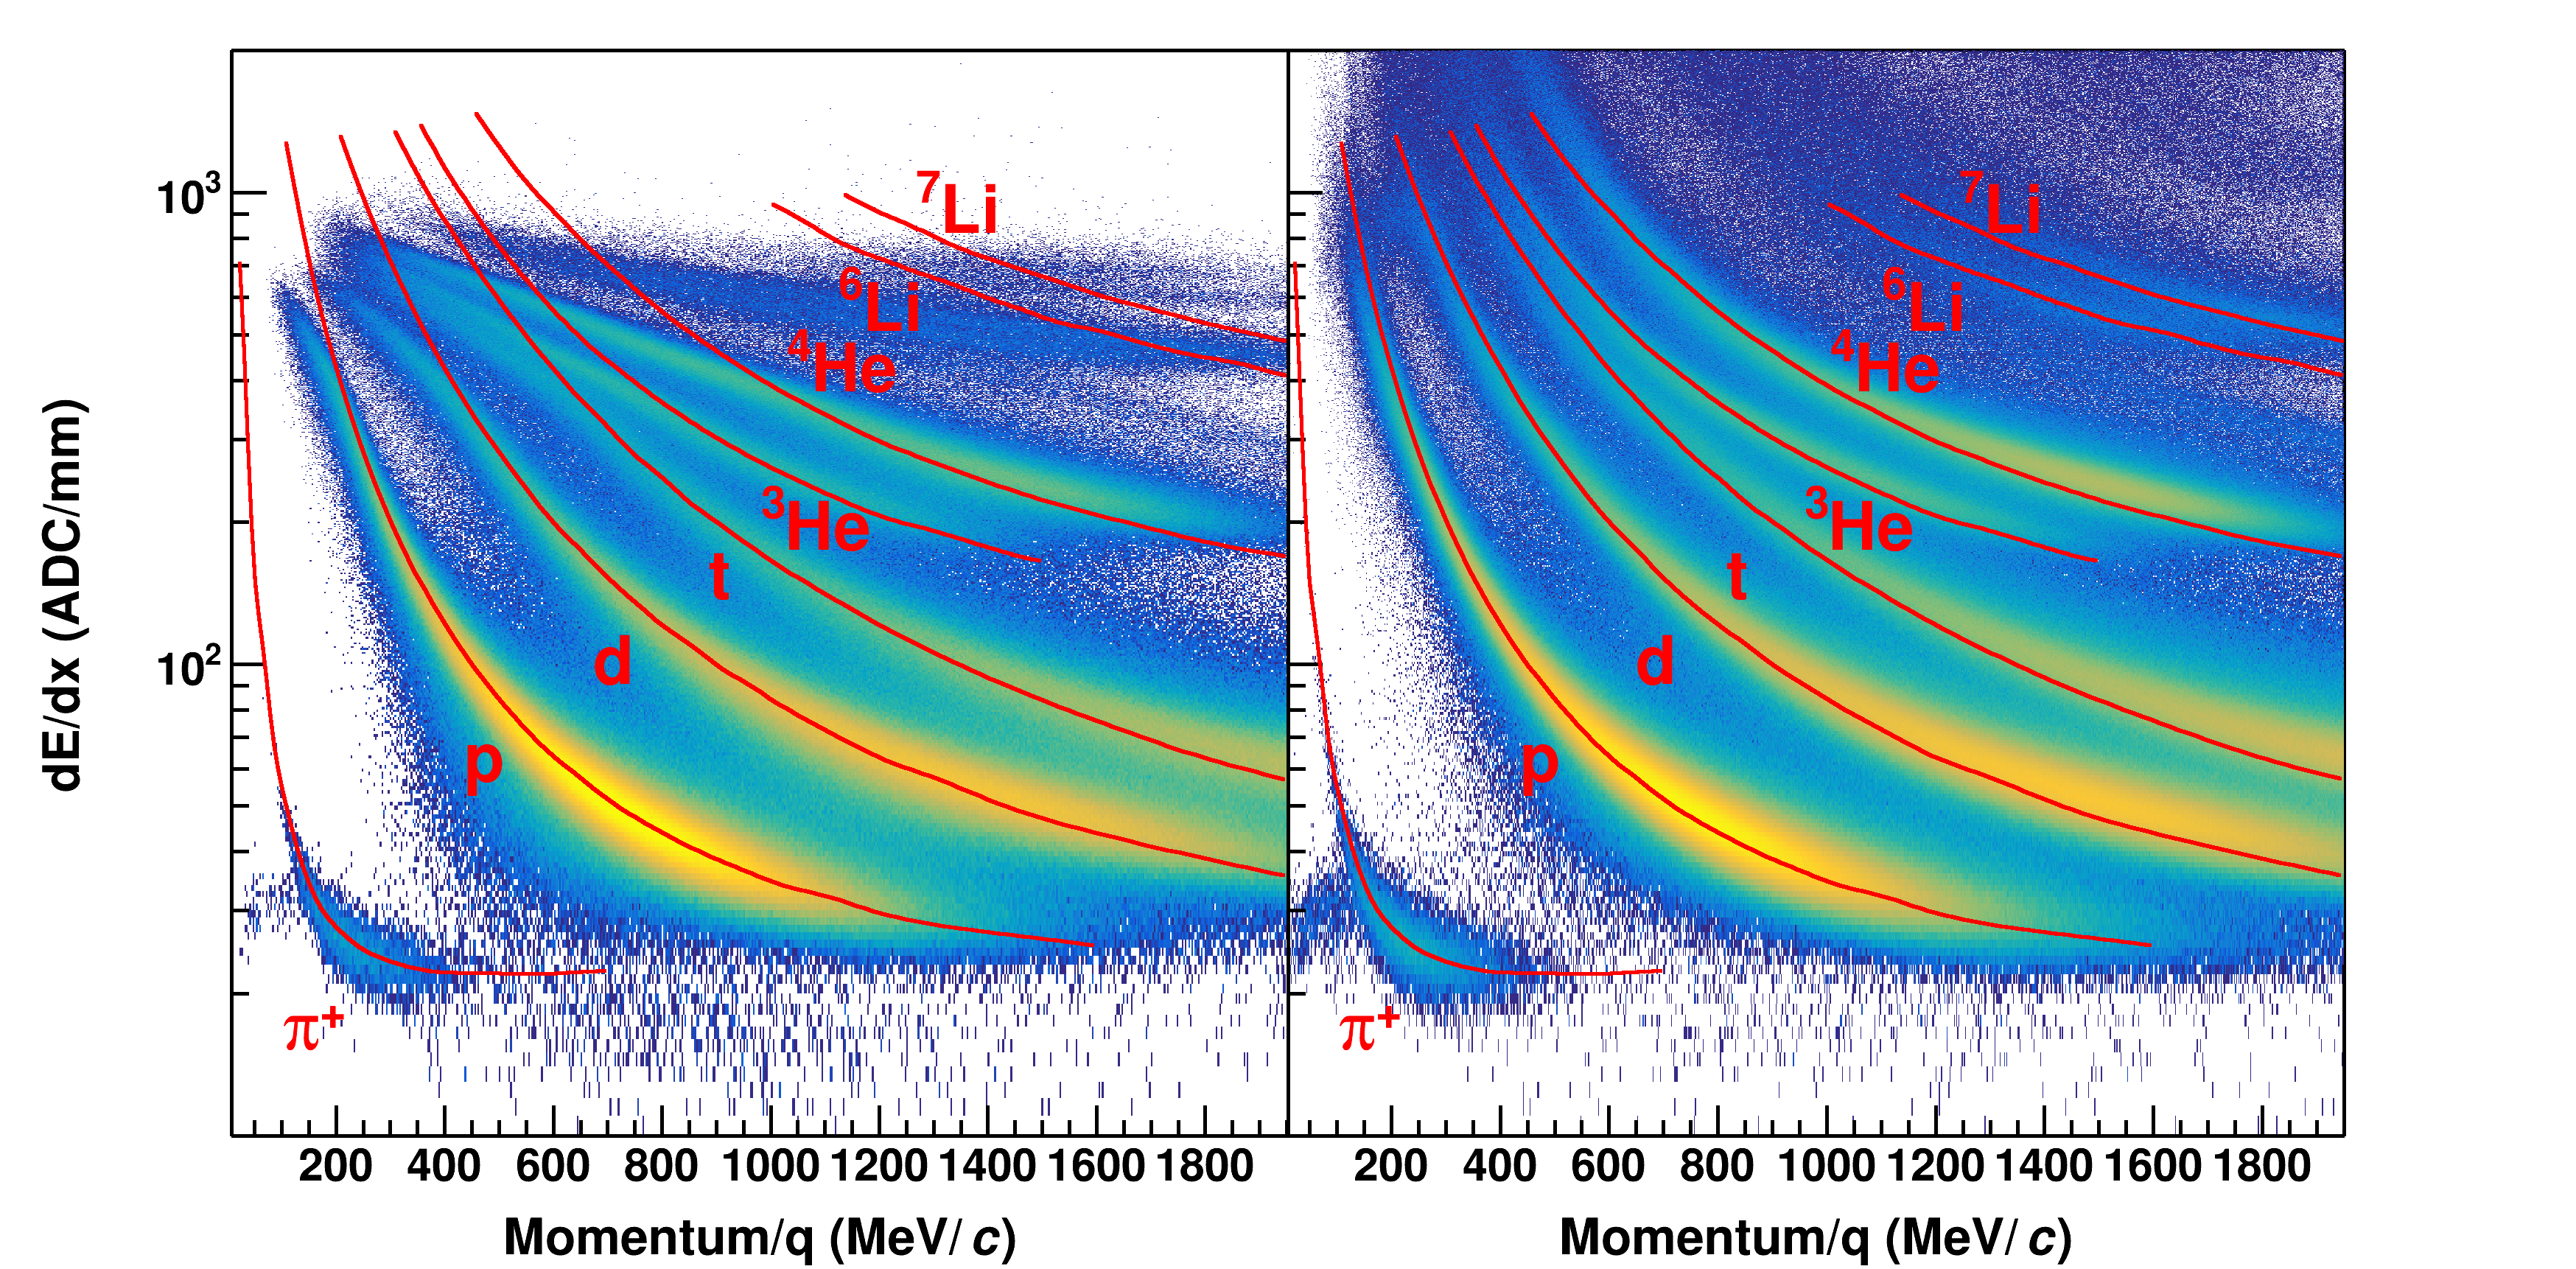
\includegraphics[width=\linewidth]{data_combine}
\caption{Uncorrected (left panel) and desaturated (right panel) collision data at polar angles of $\theta < 40^{\circ}$ and azimuthal angles between $-80^{\circ} < \phi < 80^{\circ}$}
\label{fig:data_combine}
\end{figure*}


\begin{figure*}[!htb]
\centering
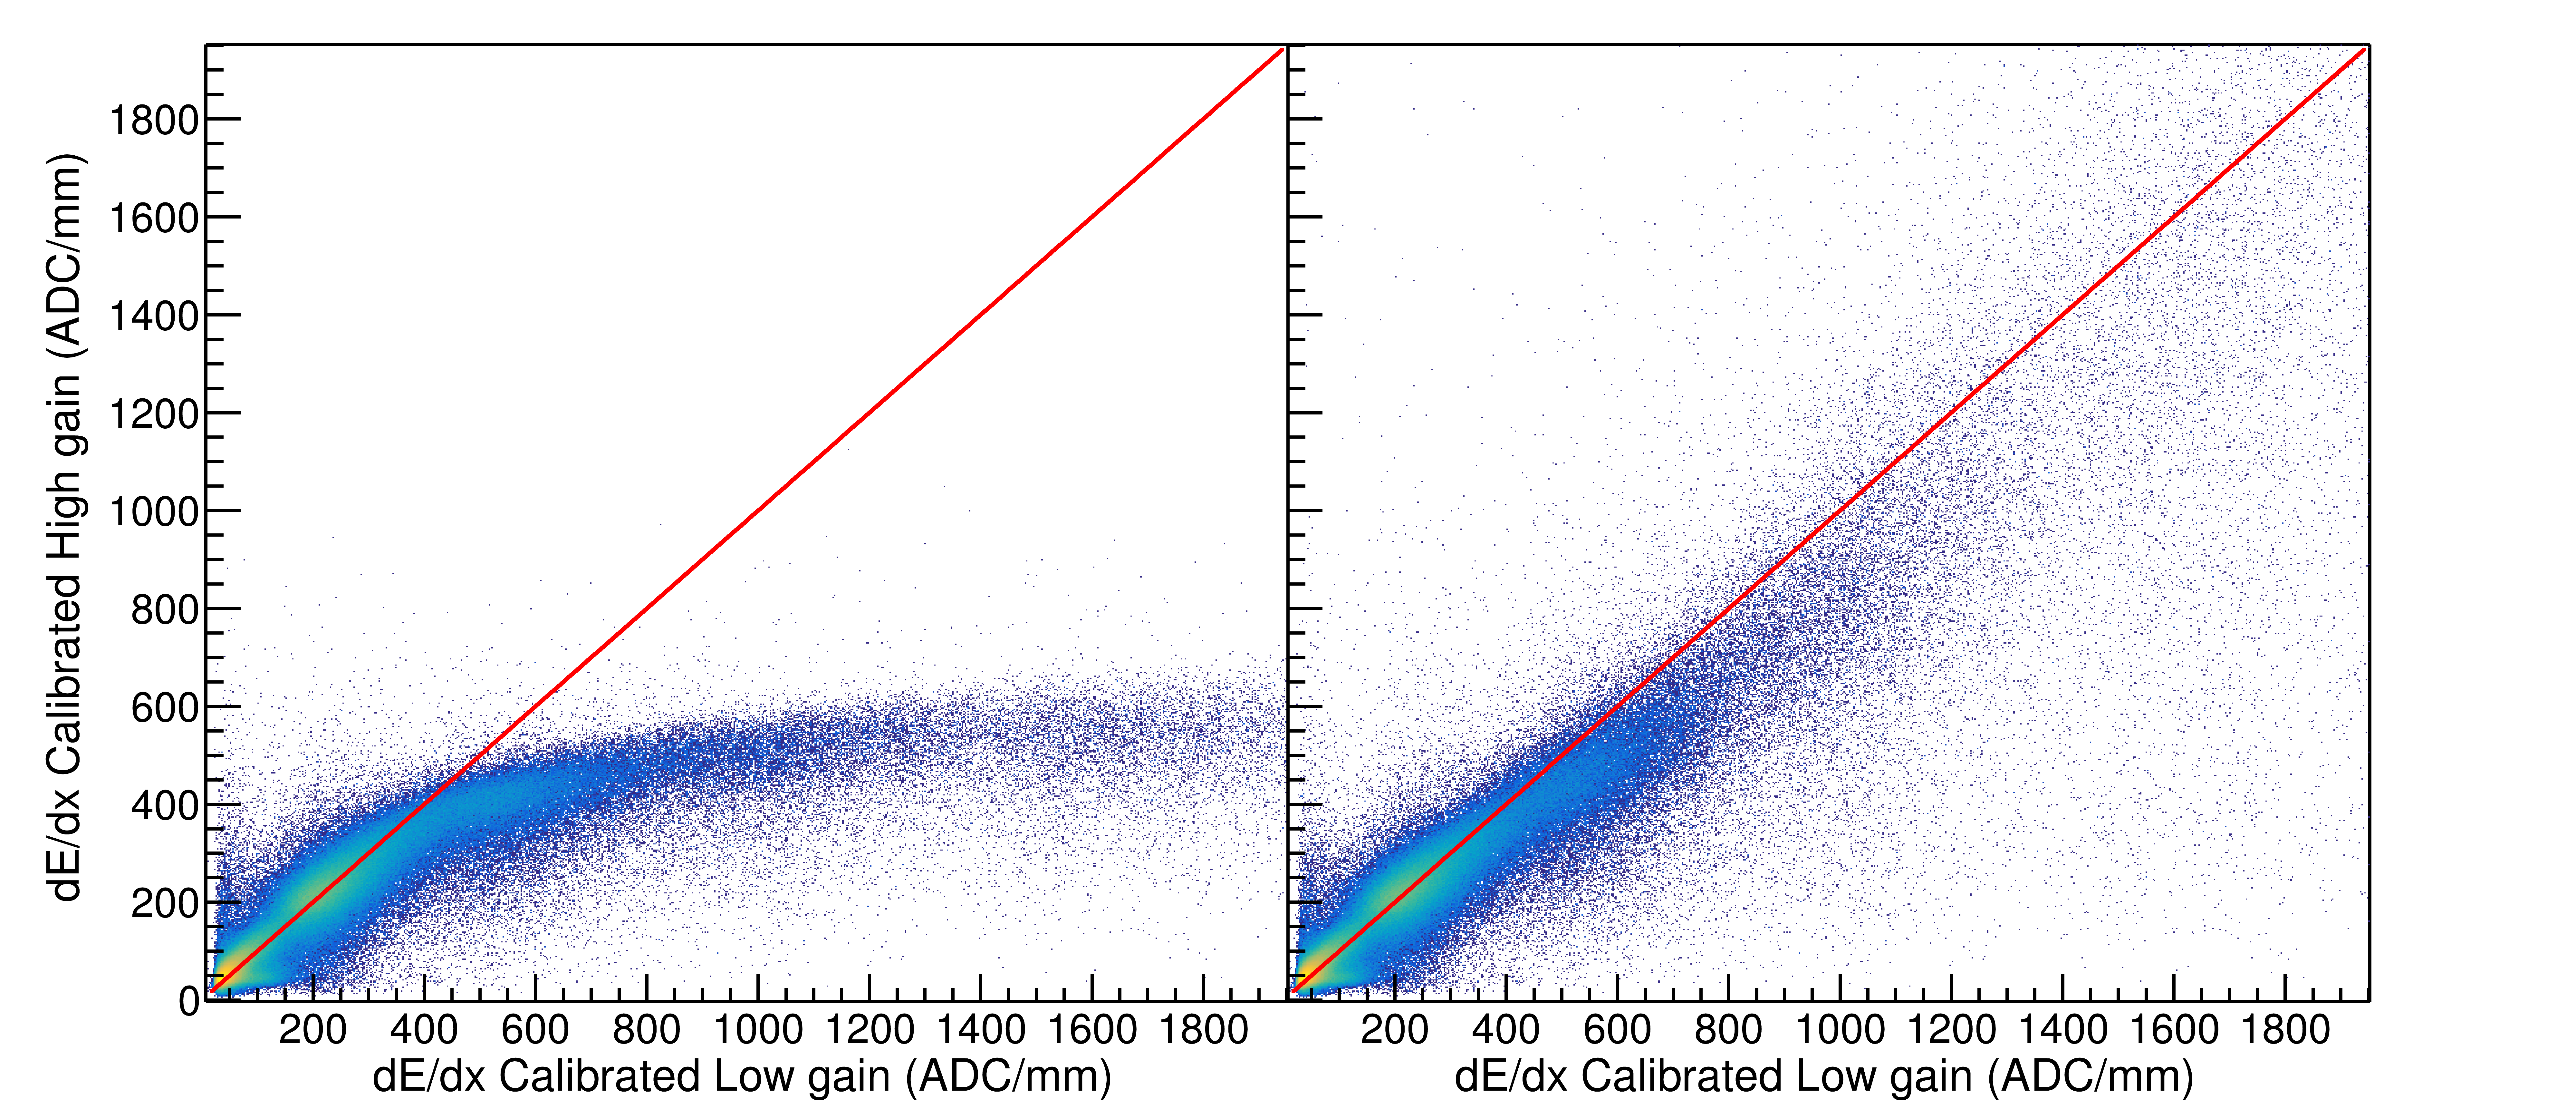
\includegraphics[width=\linewidth]{lowvshigh.png}
\caption{Uncorrected (left panel) and desaturated (right panel) collision data comparing the low gain region to the high gain anode regions of the TPC.}
\label{fig:lowvshigh}
\end{figure*}

To provide evidence of the success of this technique, we observe tracks which saturate pads in the high anode wire voltage region but are not saturated in the low anode voltage region. While this desaturation technique avoids the need to lower the gain of any region, the low anode voltage region proved to be a direct measurement of the success of this technique.
 
Figure~\ref{fig:lowvshigh} shows the $\langle dE/dx\rangle$ values of the high gain region compared with the calibrated low gain region. The effect of saturation can be seen in the high gain region for the uncorrected data above values of \SI{400}{ADC \per \milli\metre} where the values plateau, whereas the low gain region still returns accurate values. Below this value the electronics are not saturated, and therefore the high and low gain sections agree. After applying the desaturation method, the correlation between the high and low gain sections is restored, as seen in Fig.~\ref{fig:lowvshigh}. From this comparison, we can approximate that the correction has corrected the high gain sections to agree with low gain sections to values of \SI{2000}{ADC \per \milli\metre}, increasing the dynamic range by a factor of a factor of at least 5.

The success of the desaturation becomes more clear when looking at the PID lines from the experimental data in Fig.~\ref{fig:data_combine}. In the following PID plots the red lines represent the most probable energy loss as given by Geant4 straggling functions. The uncorrected data in the left panel shows the effects of saturation, where the PID lines deviate significantly from their theoretical expectations starting at around \SI{400}{ADC \per \milli\metre}. After applying the desaturation technique -- in the right panel-- we see a large improvement, most notably for the He and Li particles, which suffer the most from saturation. Even the ${}^{6}$Li and ${}^{7}$Li particles can be separated and a more subtle improvement of the lighter particles (p, d, t), can also be seen at lower momenta. In these regions, there was little to no PID resolution before desaturation technique was applied.  


%Give some failures of the assumptions made

\subsection{Space Charge Corrections}
\label{sec:spacecharge}

%MAYBE ADD A LITTLE NAPKIN CALCULATION OF SPACE CHARGE TO SHOW ORDER OF EFFECT. 

As the particles pas through the gas inside of the field cage, they ionize the gas creating electron-ion pairs. The drift velocities of the ions are typically \SI{e4} times slower than electron drift velocities \cite{blumrol}. Because of this, any source of ions have the potential to build up in the drift volume, creating a positive space charge. If the space charge build up is large enough, it would distort drifting electrons therefore biasing the track momentum measurement. There are several regions of the TPC in which ions are created. The largest source of positive ions is created in the avalanche process near the anode wires. But as discussed in Section~\ref{sec:wireplanes}, the gating grid captures all of the ions from this region. The other source of ions comes from the primary ionization produced by the beam and reaction products in the detector gas. The energy loss  $\langle dE/dx\rangle \propto Z^2$, where Z is the charge of the particle type. Because the charge of the un-reacted beam is around Z=50, the ionization due to the beam is a factor of \num{2e3} times that of the light charged particles which mostly are of charge Z=1. Therefore the ions resulting from the un-reacted beam is the largest source of positive ions in the TPC. 


%NEED TO PUT IN ABOUT THE GATING GRID LEAK 
 
 \begin{comment}
 
 \begin{table}[!htb] % not just 'h!'
\centering % not a center environment
\begin{tabular}{
  @{}
  l
  S[table-format=1.2]
  S[table-format=1.2]
  S[table-format=1.2]
  S[table-format=5.2]
  S[table-format=5.2]
  @{}
}
\toprule
Beam Energy Loss  &
 {${}^{132}$Sn} &
 {${}^{124}$Sn} &
 {${}^{112}$Sn} &
 {${}^{108}$Sn} &
  {Avg.}\\
  
\midrule
$\si{\kilo\eV\per\centi\meter}$ & 11.2   &.034  &5.43   &  903   &150     \\
\bottomrule
\end{tabular}

\caption{Average energy loss of each beam.}
\label{tb:beameloss}
\end{table}
\end{comment}


\begin{figure}[!htb]
\centering
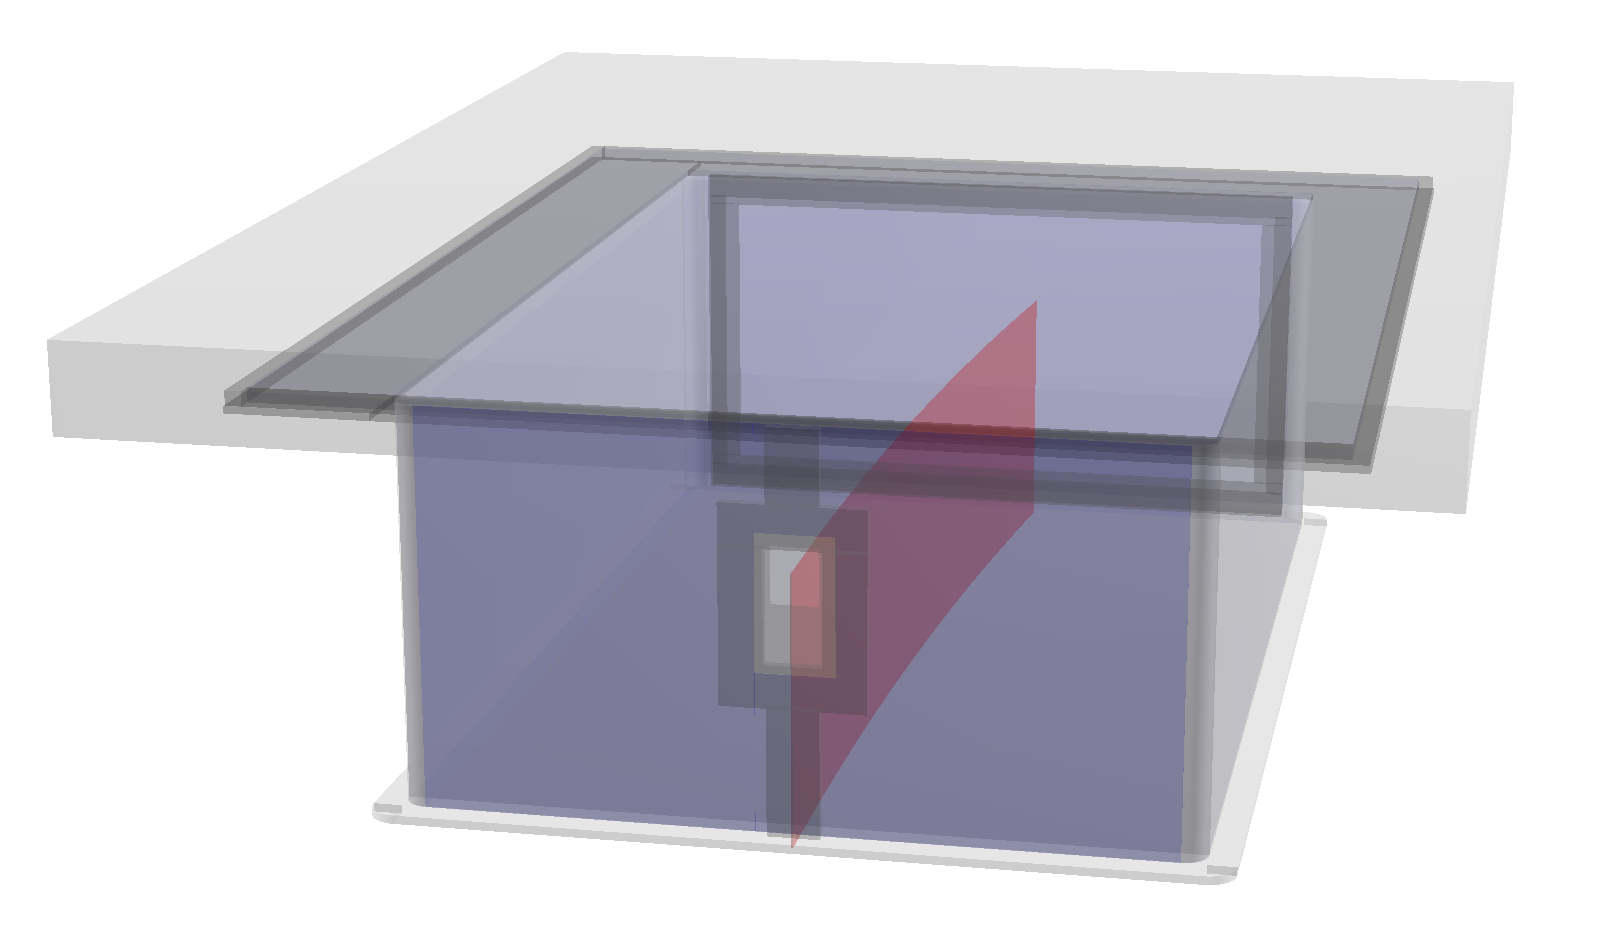
\includegraphics[width=\linewidth]{spacechg_cartoon.png}
\caption{Cartoon diagram of the location of space charge for the ${}^{132}$Sn beam.}
\label{fig:spacechg_cartoon}
\end{figure}


\begin{figure}[!htb]
\centering
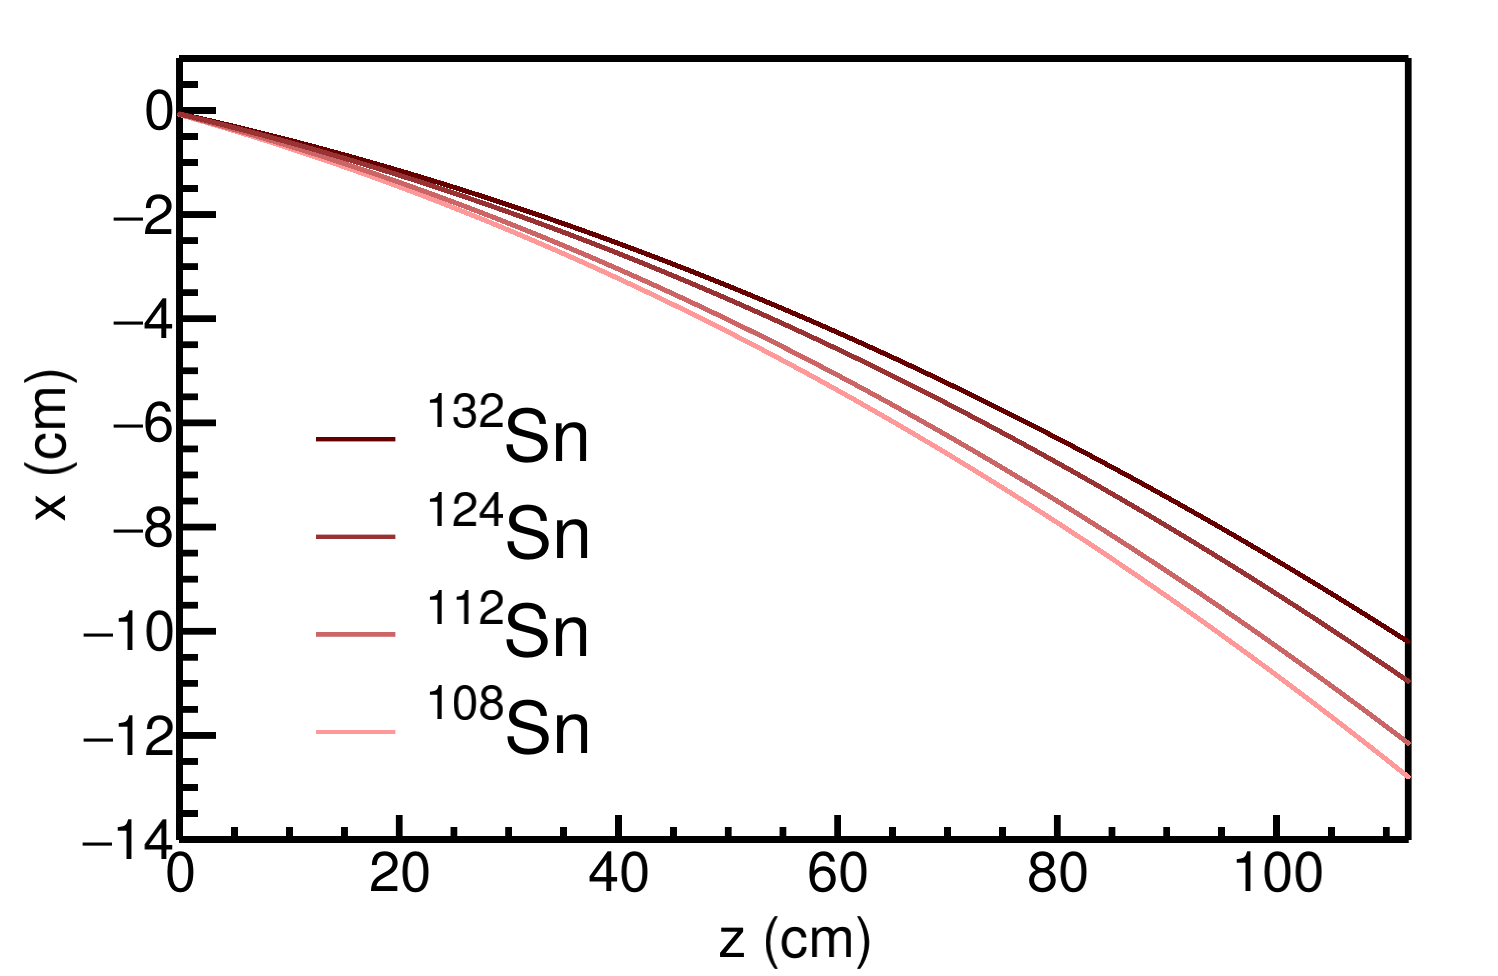
\includegraphics[width=\linewidth]{beampath.png}
\caption{Beam path of the experiments}
\label{fig:beampaths}
\end{figure}
 
 
 The beam is positioned about \SI{25}{\centi\metre} below the anode plane and \SI{29.6}{\centi\metre} above the cathode in the TPC. It takes electrons approximately 5\si{\micro\sec} to drift to the anode plane whereas it takes the ions \num{5e4}\si{\micro\sec} to drift to the cathode. The beam rate in the experiment was approximately \SI{10}{\kilo\hertz}, which has an average occurrence of 1 beam every \SI{100}{\micro\sec}. This is  much shorter than the time it takes for the ions to terminate on the cathode plane, resulting in a build up of positive ions. Figure~\ref{fig:spacechg_cartoon} gives an idea of the shape of the sheet of space charge carved out by the beam path. Figure~\ref{fig:beampaths} show the beam paths of all beams as extracted from the data. The ions from each beam create a line charge which drifts towards the cathode with a constant velocity. The average distance between sequential ion paths is about \SI{25}{\micro\metre} apart, therefore we expect the average number of beam paths that make up the sheet charge is around \num{1440} tracks. Since the number of tracks in the sheet charge is large, and inter beam spacing is very small, we approximate the sheet charge as a uniform charge density. 
 
 The secondary beams entering the TPC are also composed of many secondary species which are impurities as will be discussed in Section~\ref{sec:beam}. Their charge values are mostly distributed around Z~50. Let us assume a beam of ${}^{132}$Sn where the energy loss in P10 gas, at \SI{270}{\MeVA}, is \SI{11.2}{\kilo\electronvolt\per\centi\metre}. From the total number of beams above, and the beam path length of \SI{135}{\centi\metre}, the estimated charge density would be on the order of \SI{3e-8}{\coulomb\per\metre\squared}. This gives us an understanding of the amount of space charge we should expect to see in the chamber. 
 

Once the amount of charge is known, the electric potential can be calculated by solving Poisson's equation, 

\begin{equation}
\nabla^2 \phi = \rho,
\end{equation}

 where $\phi$ is the electric potential and $\rho$ is the free charge. The numerical solution is provided by the Jacobi method \cite{poisson}, provided all 6 sides have defined Dirichlet boundary conditions for the potentials. We neglect the wire plane region since the drift details around it are not significant for the space charge effects we are discussing here. The pad plane and cathode are trivial, where the side walls of the field cage are given linearly varying potentials on the surface, such that the electric field is the same strength as the real TPC with no space charge present. Once the electric potential is solved, the electric field is simply the gradient of the potential  $\vec{E}= -\nabla \phi$. 
 
It has been shown before that the amount of space charge present in the chamber is related to observables such as the Distance-Of-Closest-Approach (DOCA) of each track to the vertex point \cite{starSC}. In the presence of no space charge, the DOCA distribution of each track would be a centered around the true vertex location. Because of the left right symmetry in the TPC, the space charge affects different regions of the TPC differently, and a bias is introduced to the measured vertex location and widening the distribution to vertex of each track.  

An example of the distortion map in the TPC is shown in Fig.~\ref{fig:sc_shift} where left-going tracks are shown in blue, and right-going tracks shown in green. The vectors show the direction of electron shift, and their magnitude have been magnified to show the detail. The dashed lines show the tracks under the influence of the space charge where left and right-going tracks are affected differently. Right-going tracks tend to higher momentum values and the left-going tracks going to lower momentum values, for positively charged particles.  
 

\begin{figure}[!htb]
\centering
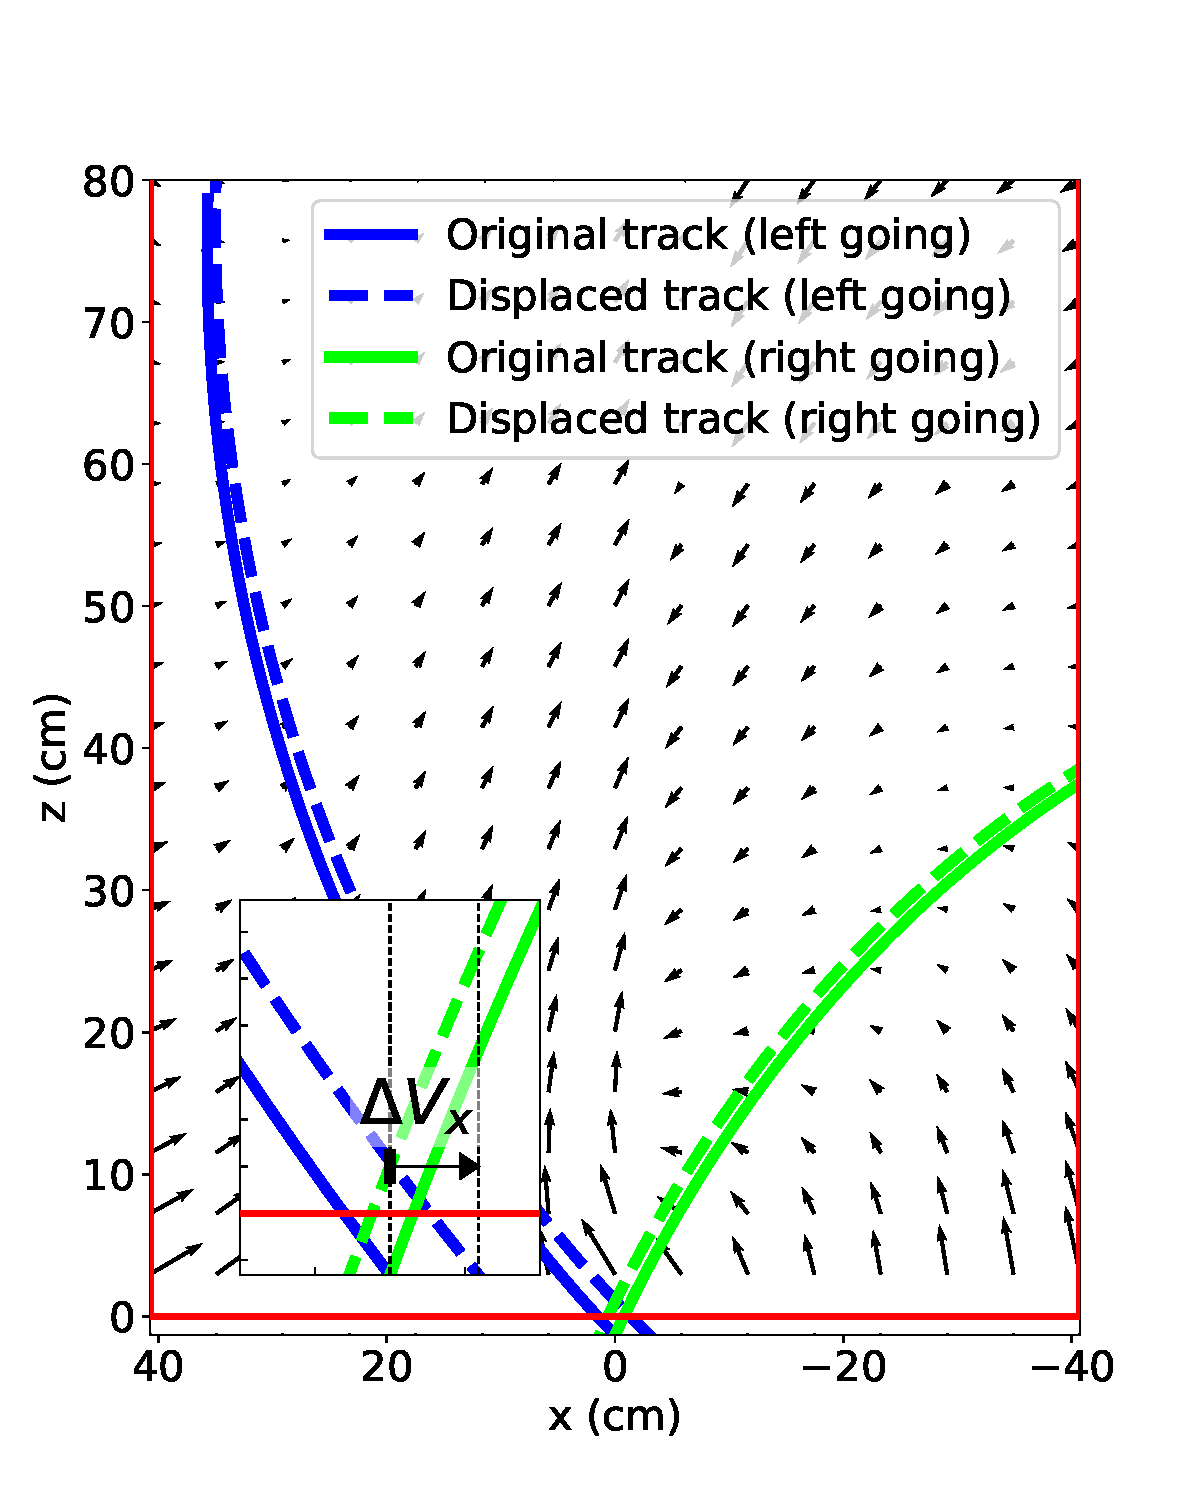
\includegraphics[scale=.5]{Effect_SC.pdf}
\caption{Example of the map of the electron shift. The effect is also shown on left-going (blue) and right-going (green) tracks. The original tracks are shown in the solid line and the shifted track in the dotted line.}
\label{fig:sc_shift}
\end{figure}

The inset figure of Fig.~\ref{fig:sc_shift} shows the effects of the space charge have on the x-component of the DOCA to the vertex. The DOCA distribution is displaced left-going track labeled by $\Delta\mathrm{V}_\mathrm{x}$, and in the opposite direction for right-going tracks. Figure~\ref{fig:VLR} shows the difference between right and left tracks as $\Delta\mathrm{V}_\mathrm{LR} = \Delta\mathrm{V}_\mathrm{x}^L - \Delta\mathrm{V}_\mathrm{x}^R$ , where  $V_x^L$ and $V_x^R$ are the most probable values of the DOCA distribution for left and right-going tracks respectively. As the space charge increases this value increases, where in the presence of no space charge, we would expect exactly $\Delta\mathrm{V}_\mathrm{LR} = 0$. 

\begin{figure}[!htb]
\centering
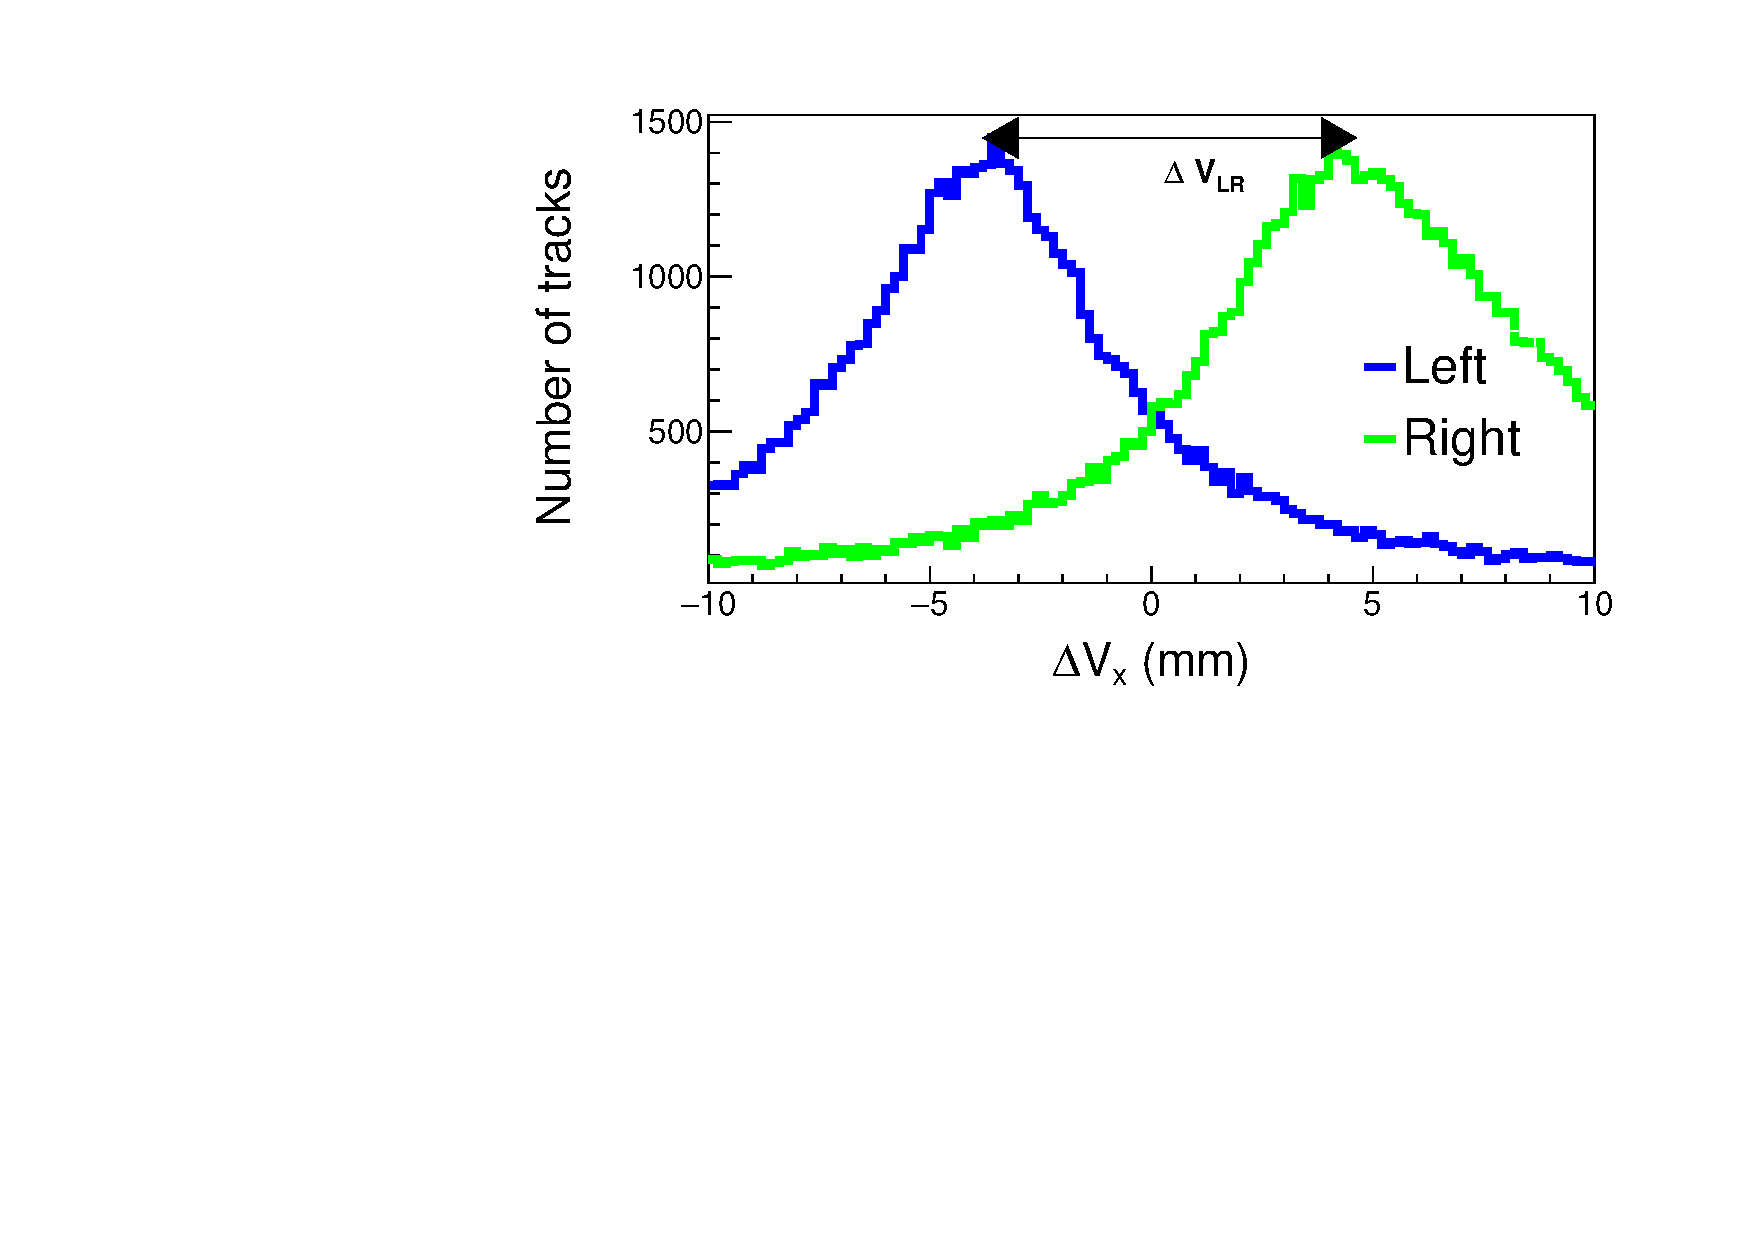
\includegraphics[scale=.5]{DVTP_raw.pdf}
\caption{$\Delta\mathrm{V}_\mathrm{x}$ distribution for left-going and right-going tracks. }
\label{fig:VLR}
\end{figure}



\begin{figure}[!htb]
\centering
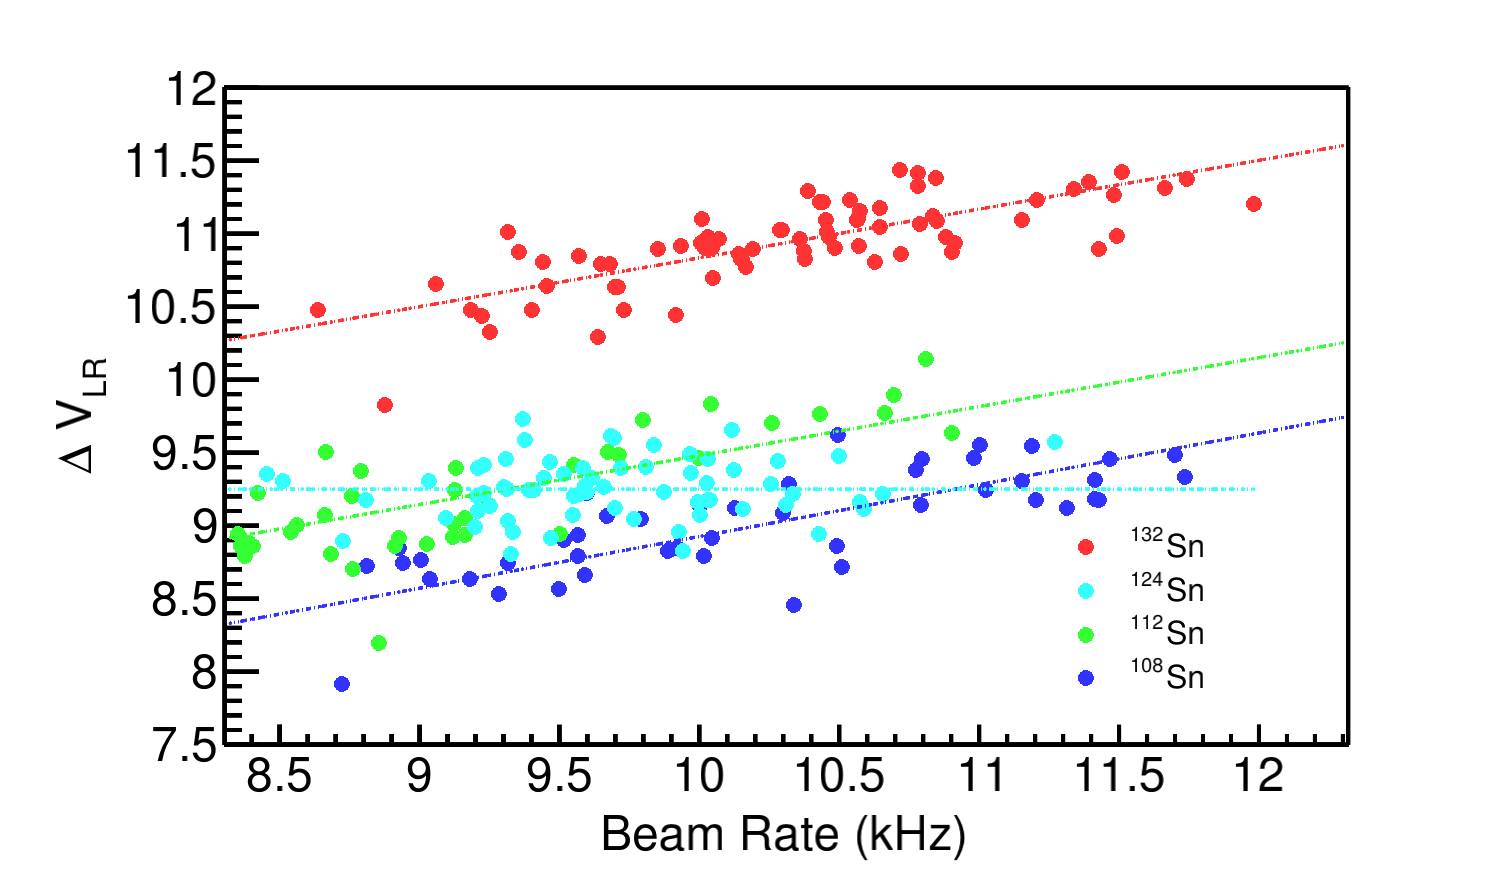
\includegraphics[width=\linewidth]{VLR_beamrate.png}
\caption{ $\Delta V_{LR}$ versus the beam rate for all systems with the fitted function.}
\label{fig:VLR_br}
\end{figure}



\begin{figure}[!htb]
\centering
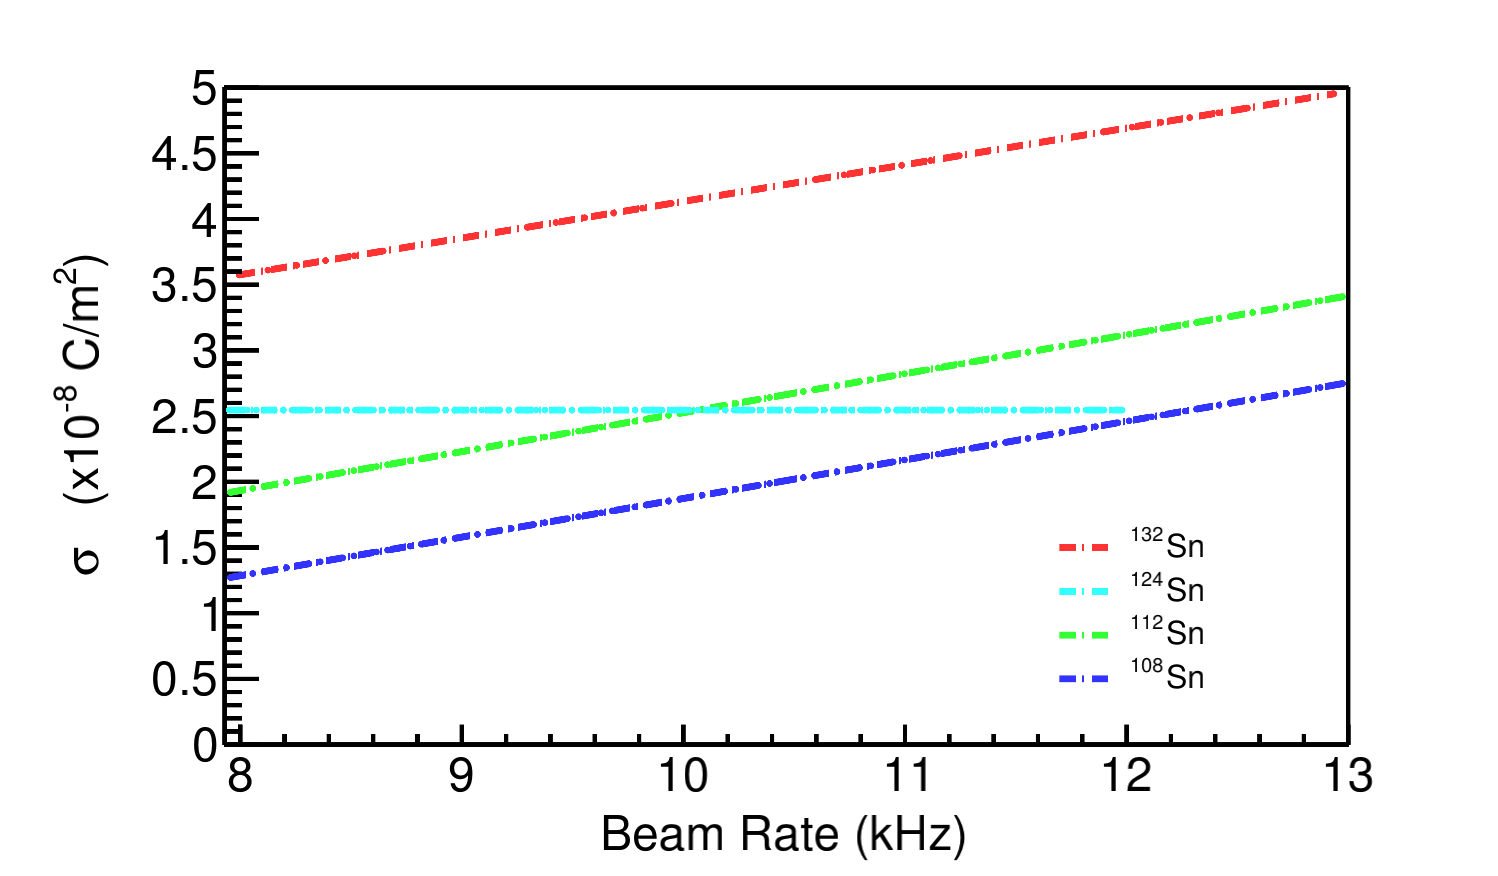
\includegraphics[width=\linewidth]{sc_beamrate.png}
\caption{Space charge fit function versus the beam rate for all systems. These are the assumed functions we use for interpolating the space charge value from the beam rate.}
\label{fig:spacechg_br_all}
\end{figure}

The average beam rate was recorded in each experimental run and slightly varied from run to run due to beam production variations. The amount of space charge present in the field cage is directly proportional to the beam rate and therefore $\Delta\mathrm{V}_\mathrm{LR}$.  Fig.~\ref{fig:VLR_br} shows the relation between the measured $\Delta\mathrm{V}_\mathrm{LR}$ values and the estimated beam rate. 

The only parameter in the space charge correction algorithm is the surface charge density $\sigma_{\mathrm{SC}}$. By varying $\sigma_{\mathrm{SC}}$ for a wide range of values, the $\Delta\mathrm{V}_\mathrm{LR}$ observable is measured and plotted in the left panel of Fig.~\ref{fig:spacechg_relation}. The values are linearly fit to find the solution of the surface charge density which gives $\Delta\mathrm{V}_\mathrm{LR} = 0$, which is then taken to be the estimate for the average amount of space charge present in a given run.

This is done for several runs which vary in beam intensity. Since the surface charge density is proportional to the beam rate, a linear fit gives good agreement for interpolating the surface charge values as a function of beam rate. Figure~\ref{fig:spacechg_relation} shows the relation of the dependence of the space charge as a function of beam rate for the ${}^{132}$Sn system.

\begin{figure}[!htb]
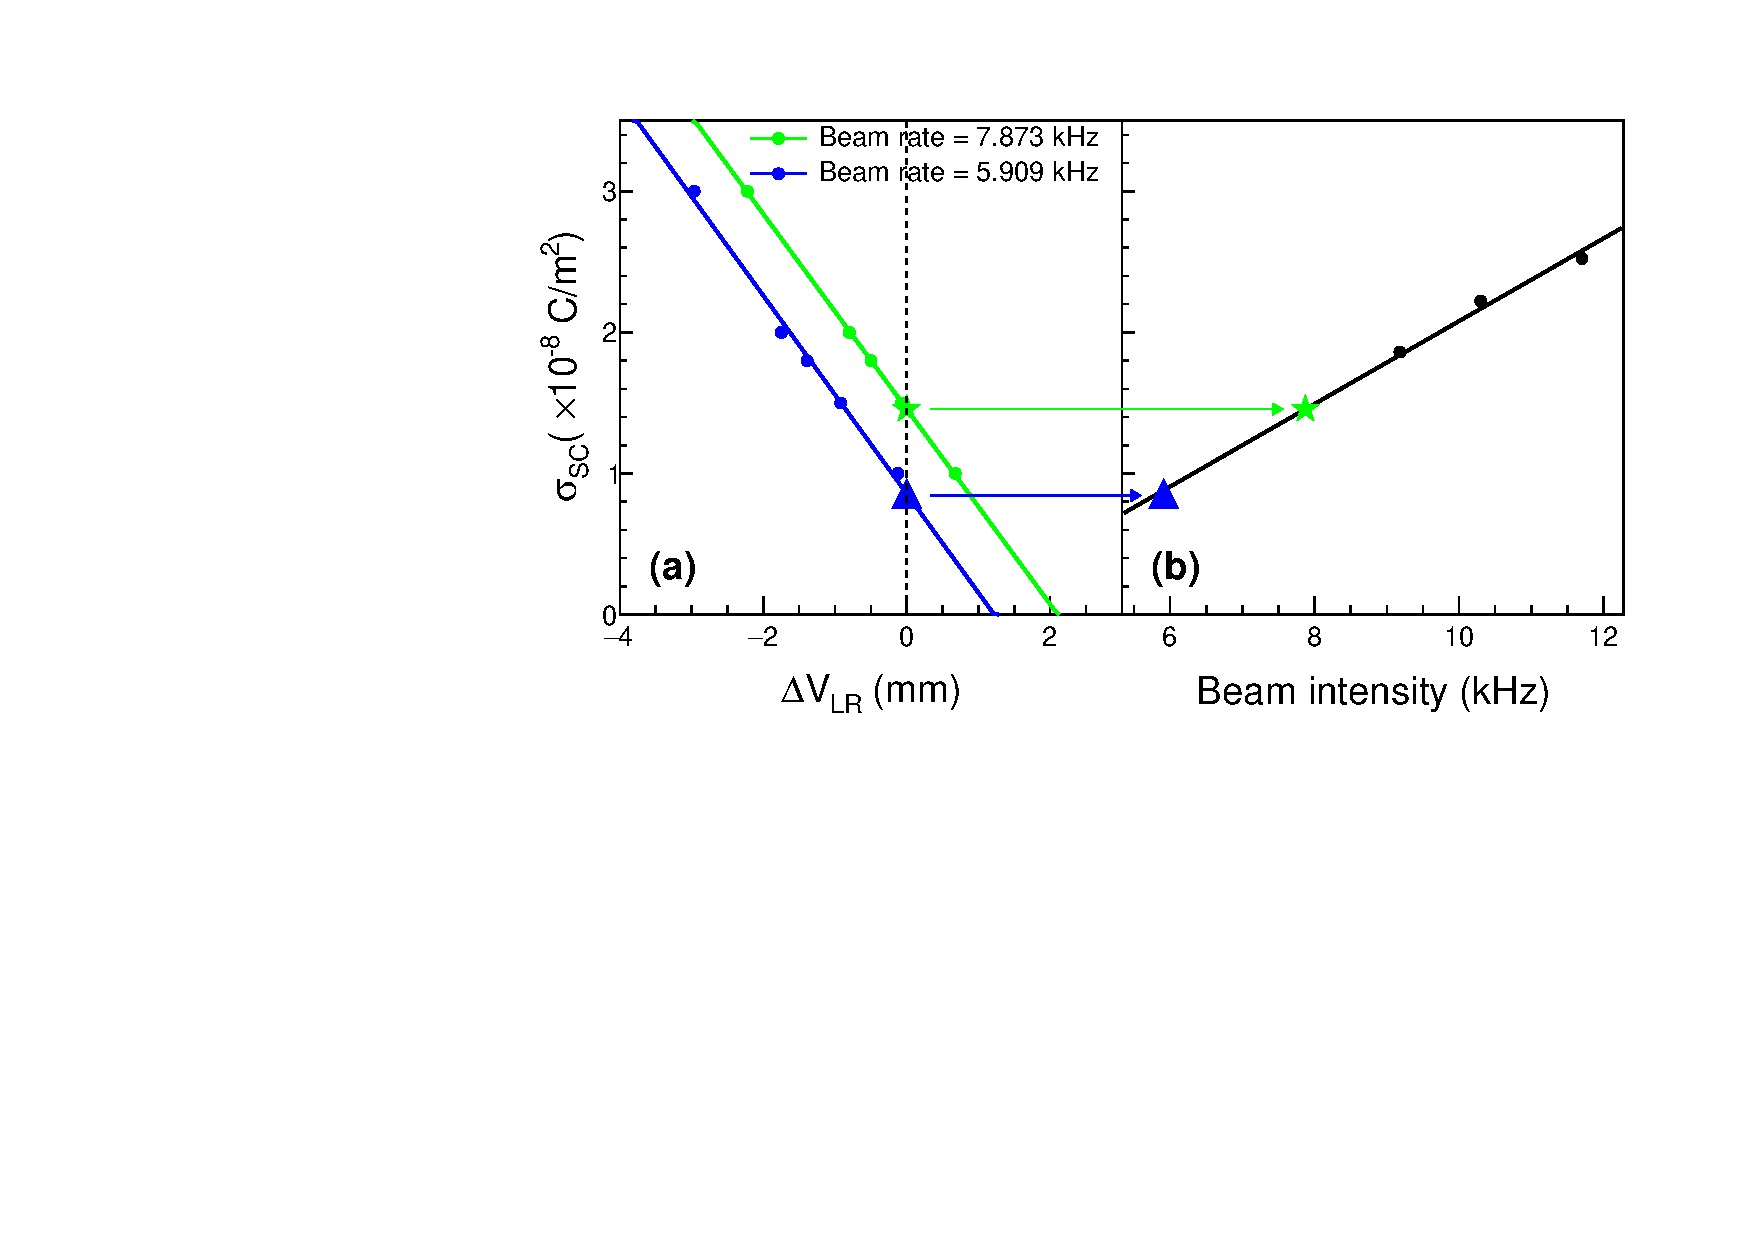
\includegraphics[width=\linewidth]{SC_Relation.pdf}
\caption{Relationship between the observable  $\Delta\mathrm{V}_\mathrm{LR}$ and the estimated charge density, and the beam intensity for each run. The blue and green line represents two separate runs at different beam intensities. The condition for  $\Delta\mathrm{V}_\mathrm{LR} = 0$ is solved for for each run. These values are then plotted against the beam intensity where finally a linear fit provides the interpolation for all beam intensities in between.}
\label{fig:spacechg_relation}
\end{figure}


Following this algorithm, the space charge can be estimated for each run and system. Figure~\ref{fig:scDensity} shows the summary of the extracted space charge values for each secondary beam. The linear fits relating the space charge density to the beam rate for each system is shown in Fig.~\ref{fig:spacechg_br_all} where the space charge value is inferred from the measured beam rate. Notice that in the $\tin{112}{124}$ system we assume a constant for the space charge density, since the variation in $\Delta\mathrm{V}_\mathrm{LR}$ rate did not span a large enough range to warrant a more detailed analysis. 

To reduce the need to compute a new electric field for each space charge value, notice that $E \propto \rho$. We can therefore solve the electric field for a certain reference charge value $\rho_o$, and scale the solution for any other free charge $\rho$ linearly by the ratio $\rho/\rho_o$. The full magnetic field map is provided by the SAMURAI collaboration \cite{magnet}. The velocity field map is calculated following Eq.~\ref{eq:elecdrift}, where the electron drift through this velocity map is propagated by using a time stepped $\mathrm{4}^{\mathrm{th}}$-Order Runge-Kutta integration from a certain starting point.
  
 The correction map is calculated in the inverse method, starting from the anode wires and location on the pad-plane (x,z), and stepping backward in time in the Runge-Kutta integration through the velocity field map until the electron reaches the measured y-position. This is done over a 3-dimensional grid where points in between are interpolated by a tri-linear interpolation. The measured clusters value (x,y,z) position is input into the correction map which outputs the interpolated correction values $dx$ and $dz$ which correspond to that cluster. The cluster position is then shifted to new positions $x\textprime = x + dx$ and $z\textprime = z + dz$.
 

%What is the best figure to put in? VLR vs Charge density? 
%estimate of the error of VLR and how it corresponds to charge density

\begin{figure}[!htb]
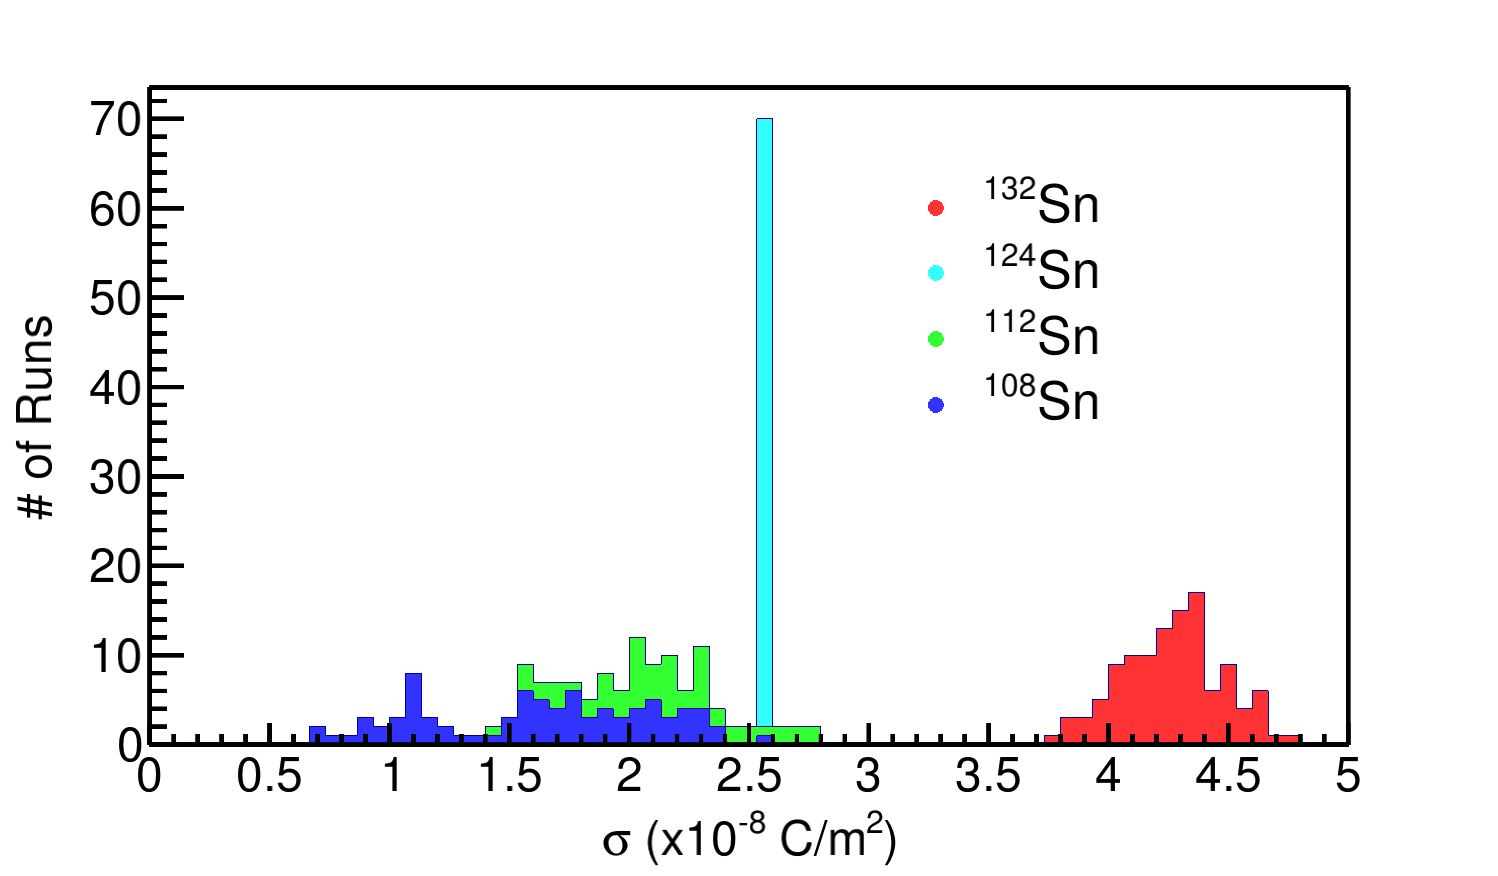
\includegraphics[width=\linewidth]{spaceChgDensity.png}
\caption{Distribution of estimated space charge densities for each beam type.}
\label{fig:scDensity}
\end{figure}



\begin{figure}[!htb]
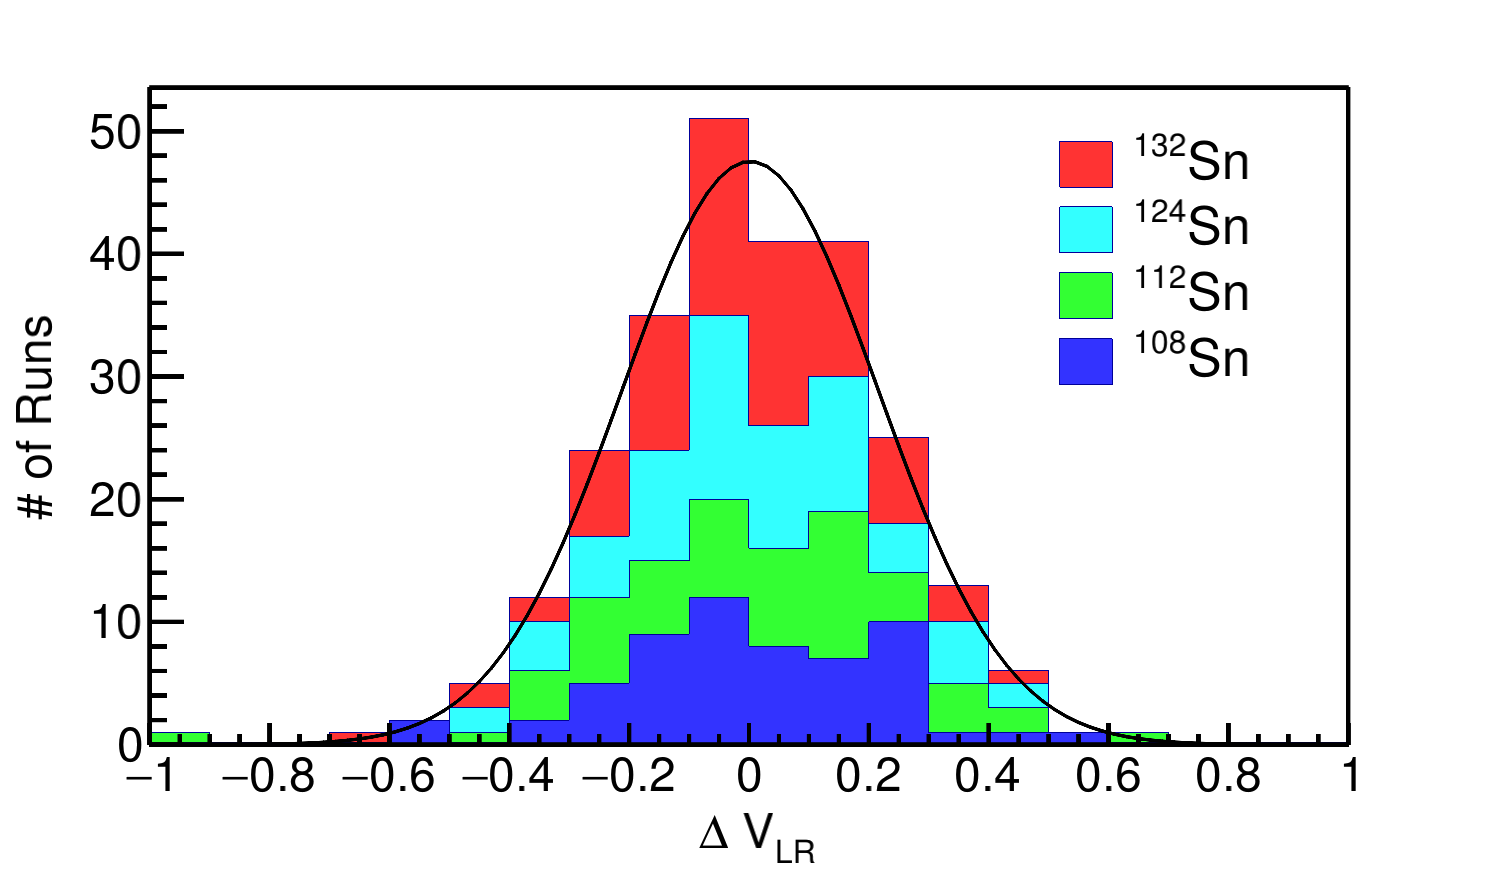
\includegraphics[width=\linewidth]{VLRresidual.png}
\caption{Residuals in the fitted line of $\Delta V_{LR}$ observable for all systems.}
\label{fig:vlrResidual}
\end{figure}

Adding the BDC vertex greatly improves the momentum resolution of the track fitting.  Since we know that the space charge affects right and left-going tracks differently, both tracks diverge from the original vertex location appearing to no longer originate from the BDC vertex which is independent of the space charge effects. Without correcting for the space charge effects adding the BDC introduces a systematic shift in the momentum when comparing right and left-going tracks as compared with the momentum value before adding the BDC. For tracks at polar angles of $\theta_{Lab} < \ang{40}$, the disagreement between momentum values with and without the BDC are much less obvious. This is because for small deviations in the track -- at smaller polar angles -- leads to small deviations at the target location. Therefore the momentum without the BDC as an extra constraint does not disagree as much with the BDC point as shown in Fig.~\ref{fig:mom_S_before}. Figure~\ref{fig:mom_L_before} shows the momentum value of tracks going at polar angles of $\theta > \ang{40}$ which are more sensitive to small changes in the track -- corresponding to larger deviations at the target location. Therefore we get large systematic shifts in the momentum after including the BDC. After correcting for the space charge effects, the reconstructed momentum value agrees with or without the BDC included, for both  polar angles $\theta_{Lab} < \ang{40}$ and $\theta_{Lab} > \ang{40}$, as seen in Fig.~\ref{fig:mom_S_after} and Fig.~\ref{fig:mom_L_after} respectively. 


\begin{figure}[!htb]%
    \centering
    \subfloat[Compare the momentum before and after including the BDC vertex for tracks with $\theta_{Lab} < \ang{40}$, before the space charge correciton.]{{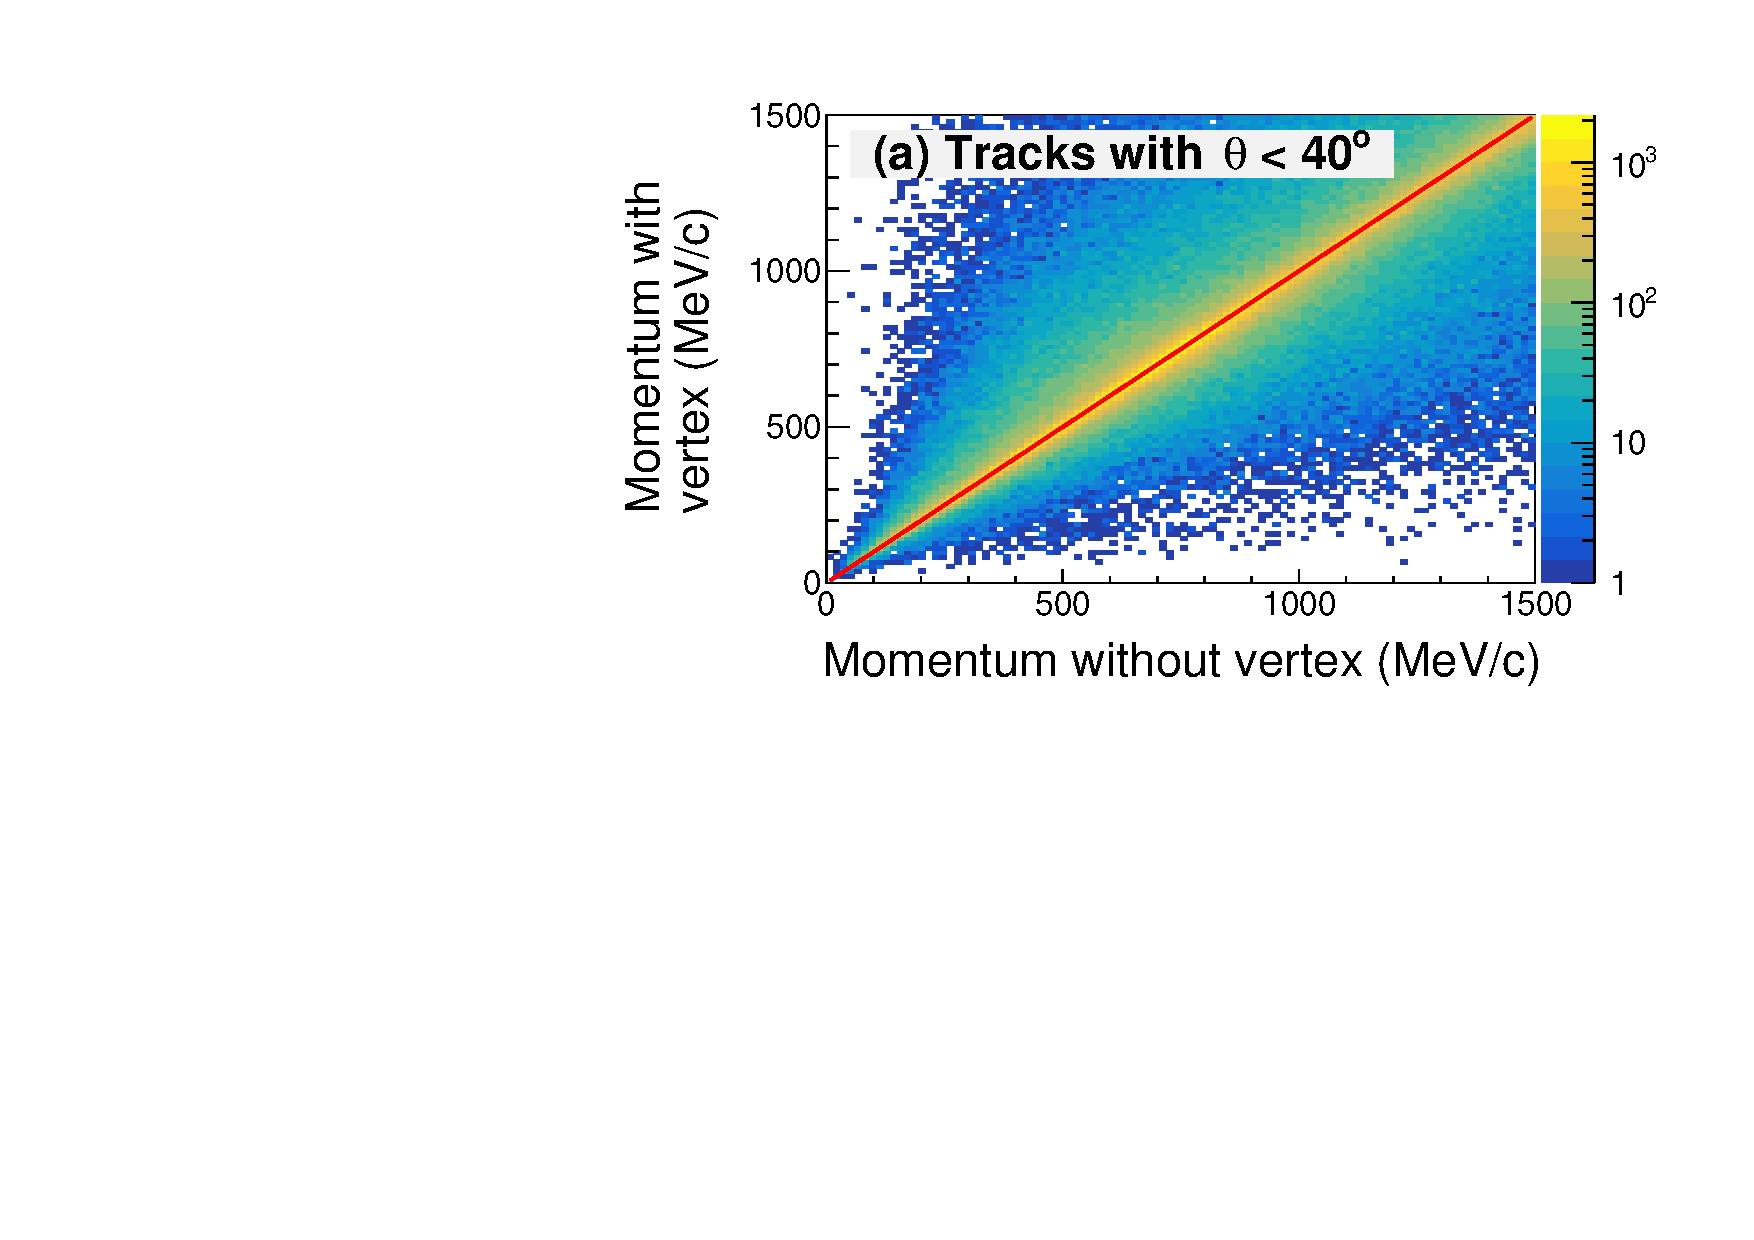
\includegraphics[width=.45\textwidth,valign=c]{BDC_P_small_angle.pdf} \label{fig:psa0}}}%
    \qquad
    \subfloat[Comparison of the momentum before and after including the BDC vertex for tracks with $\theta_{Lab} > \ang{40}$, before the space charge correction.]{{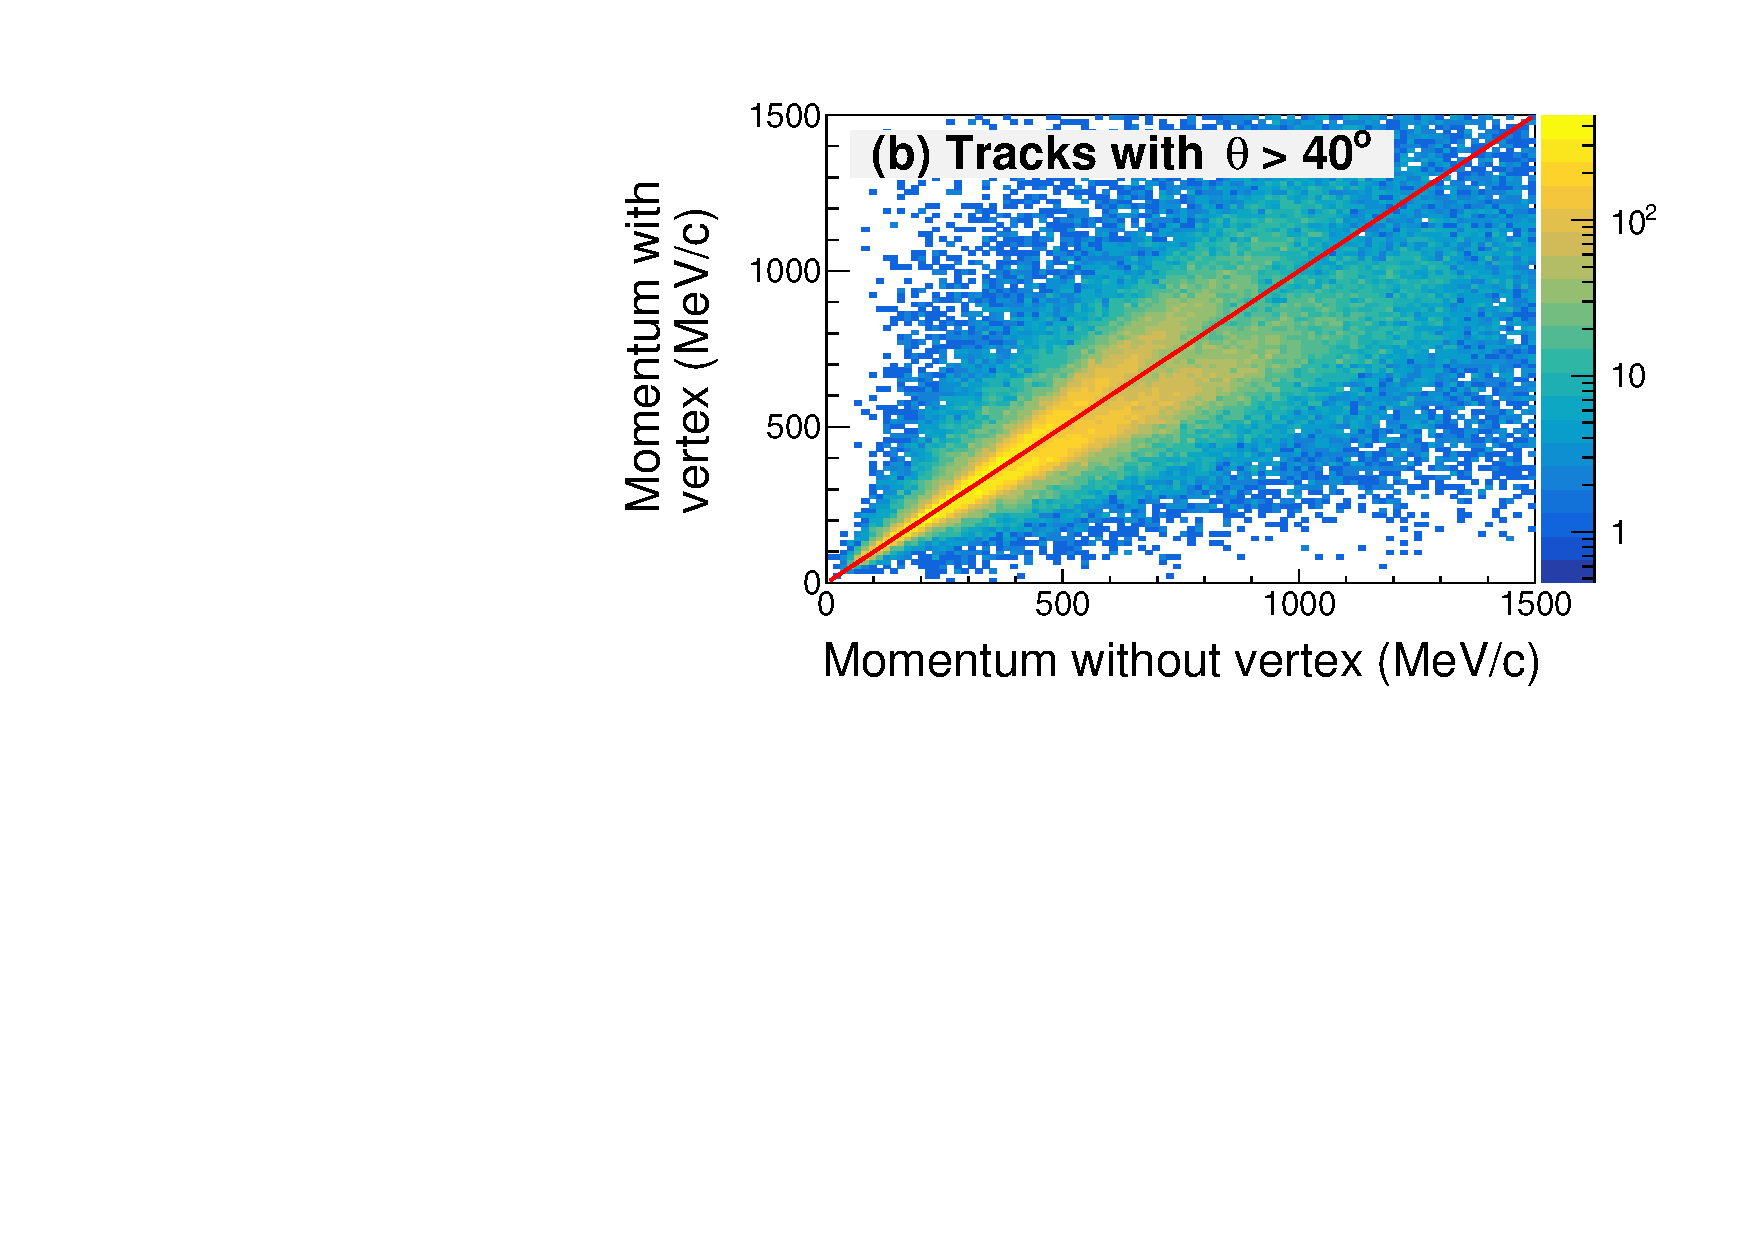
\includegraphics[width=.45\textwidth,valign=c]{BDC_P_large_angle.pdf} \label{fig:mom_L_before}}}\\
    \subfloat[Compare the momentum before and after including the BDC vertex for tracks with $\theta_{Lab} < \ang{40}$, after the space charge correction.]{{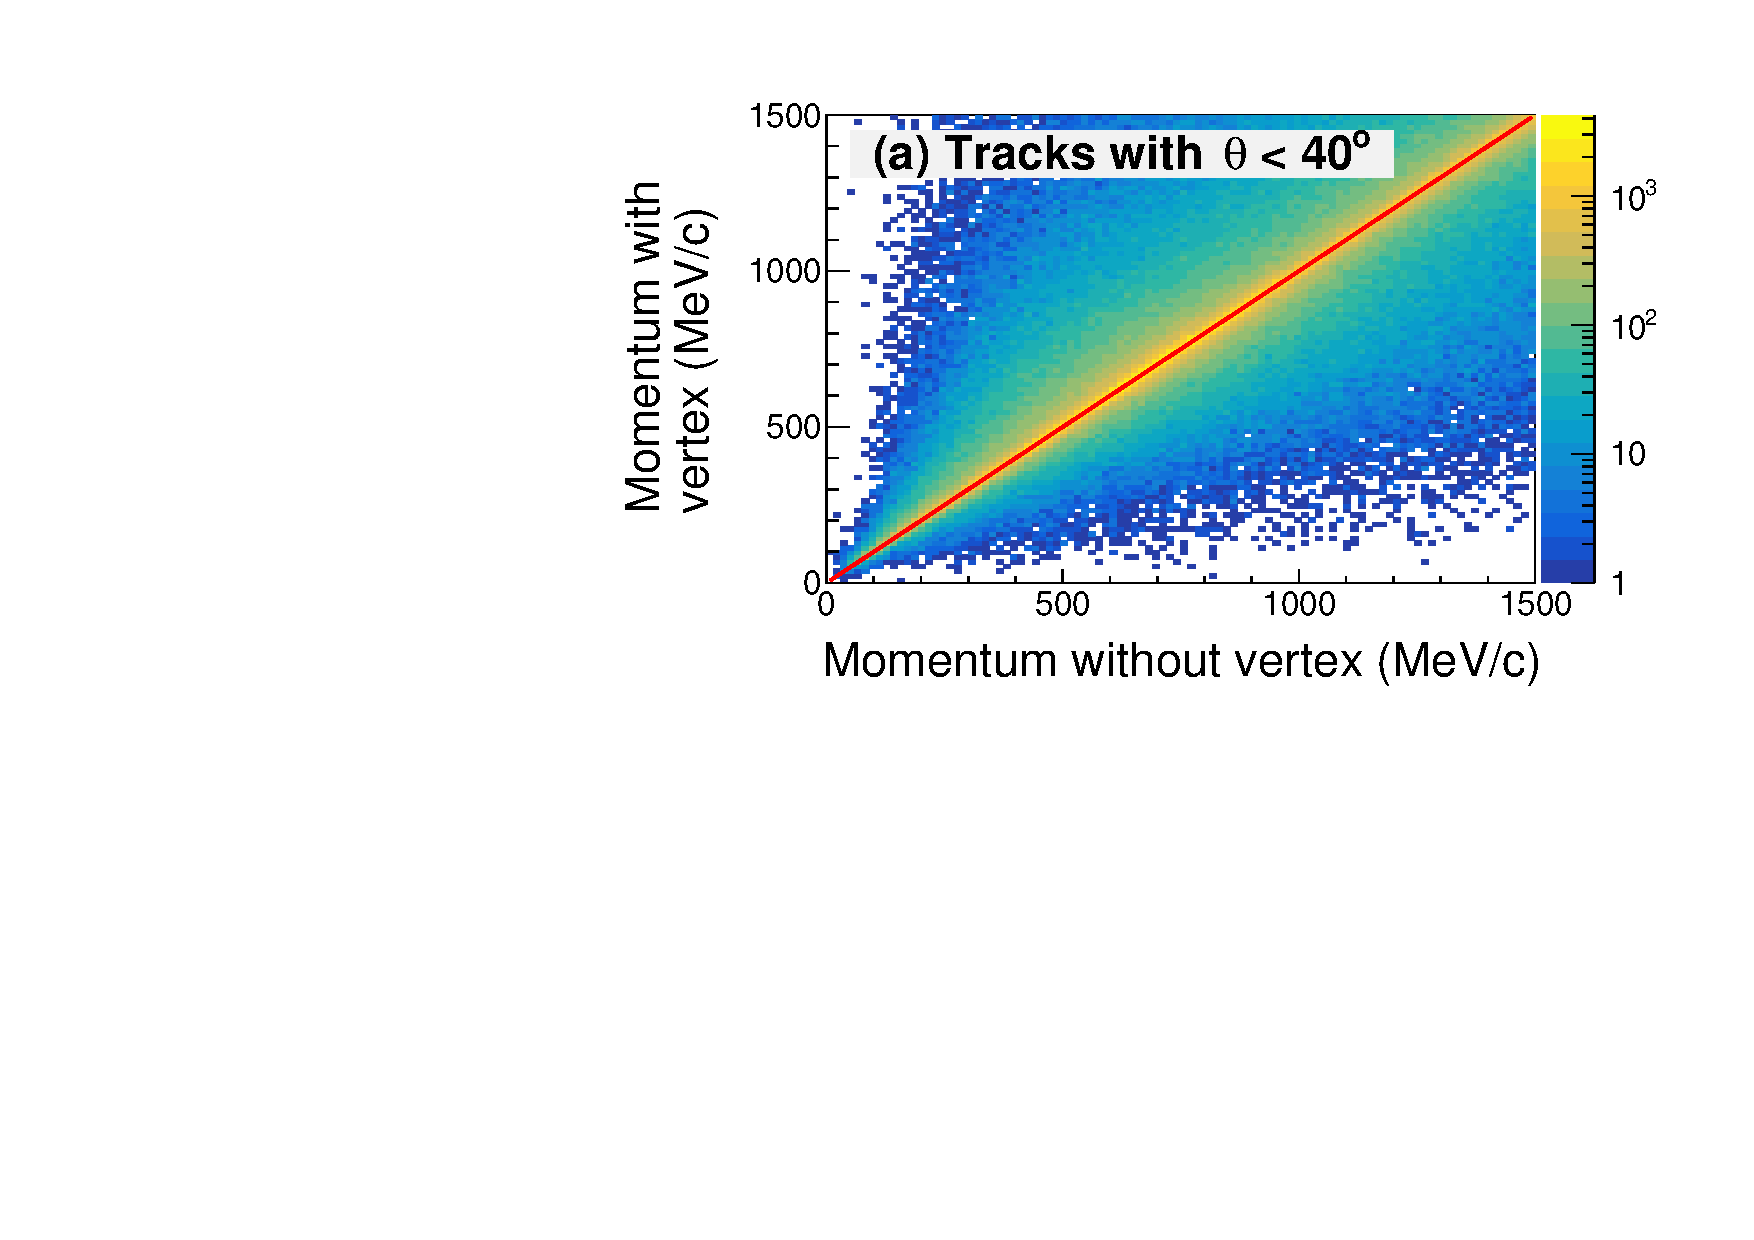
\includegraphics[width=.45\textwidth,valign=c]{BDC_P_aftercor_small_angle.pdf} \label{fig:mom_S_after}}}%
    \qquad
    \subfloat[Compare the momentum before and after including the BDC vertex for tracks with $\theta_{Lab} < \ang{40}$, after the space charge correction.]{{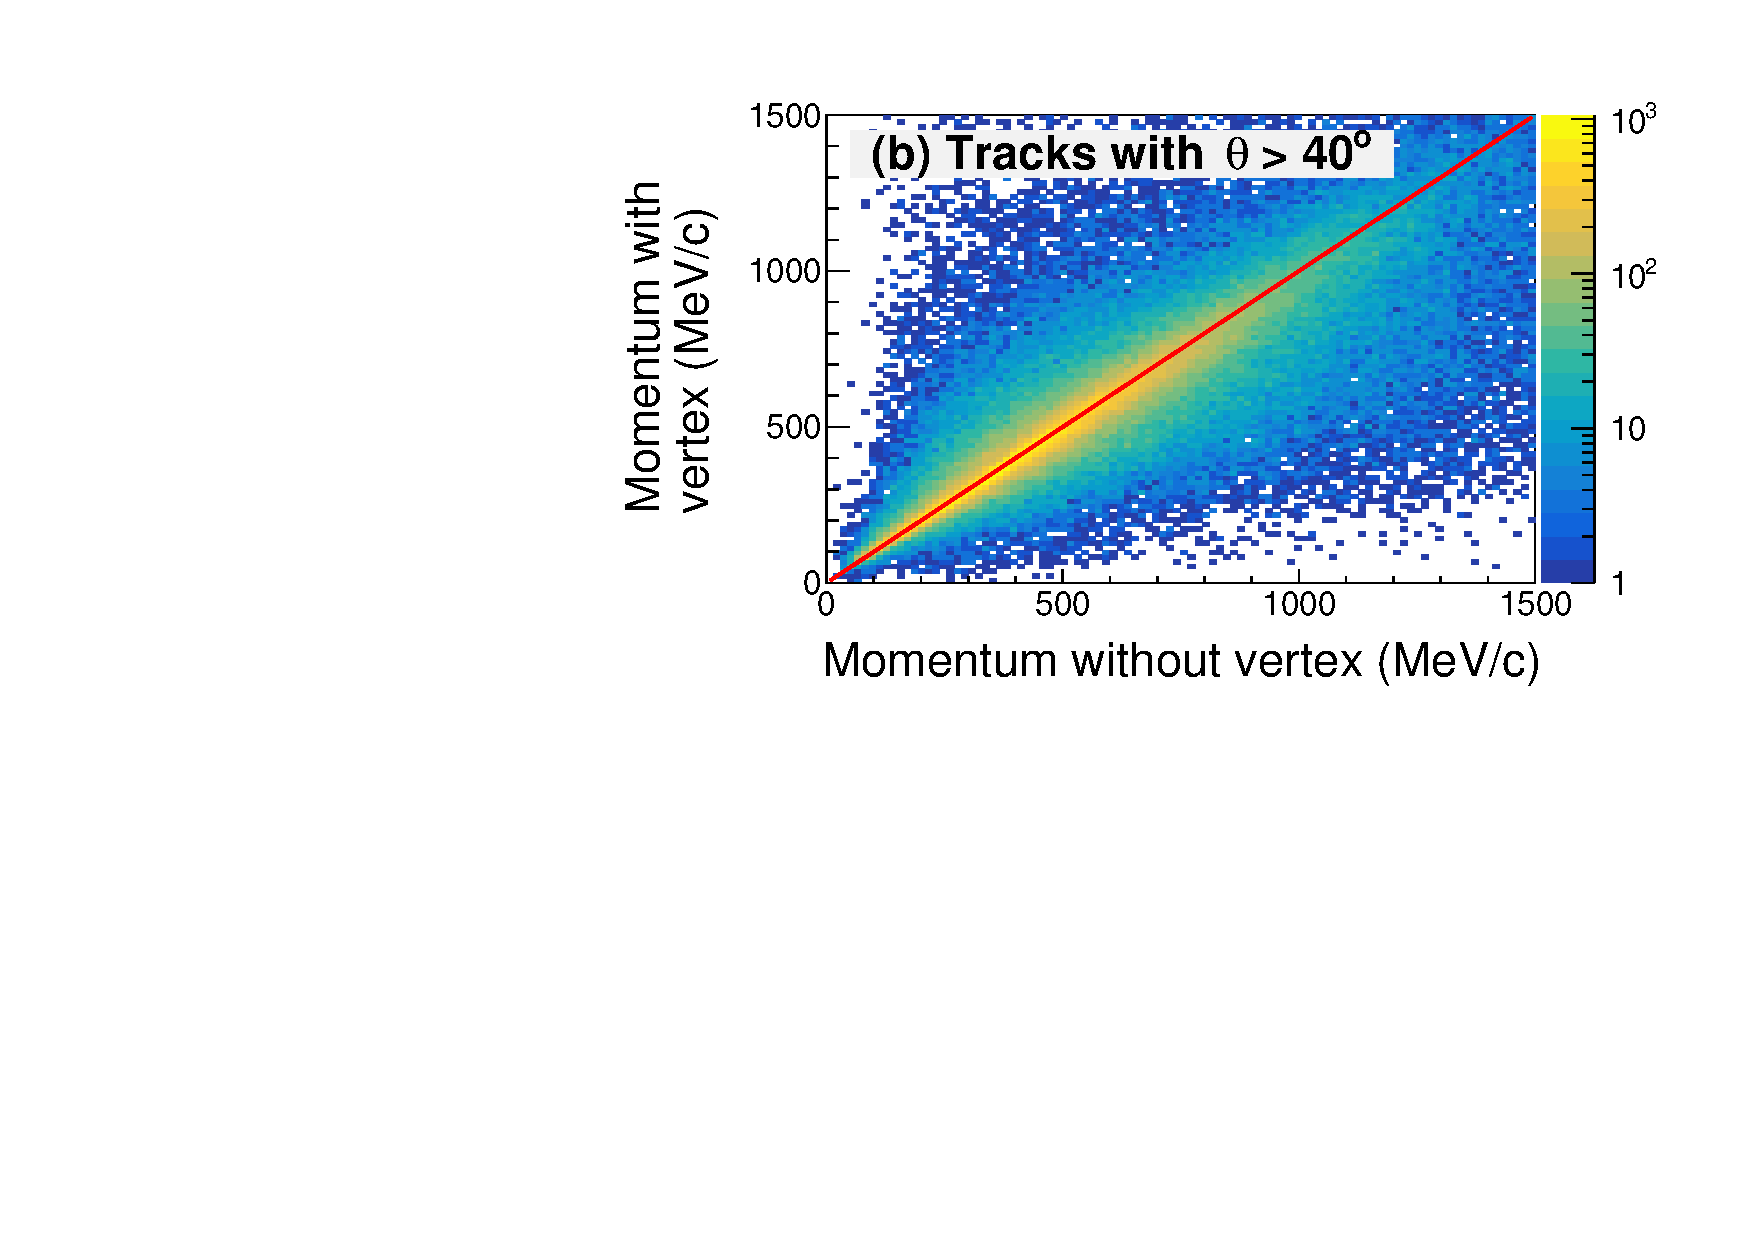
\includegraphics[width=.45\textwidth,valign=c]{BDC_P_aftercor_large_angle.pdf}  \label{fig:mom_L_after}}}%

 \label{fig:mom_sc}
\end{figure}



\begin{figure}[!htb]%
    \centering
    \subfloat[$\tin{132}{124}$ system.]{{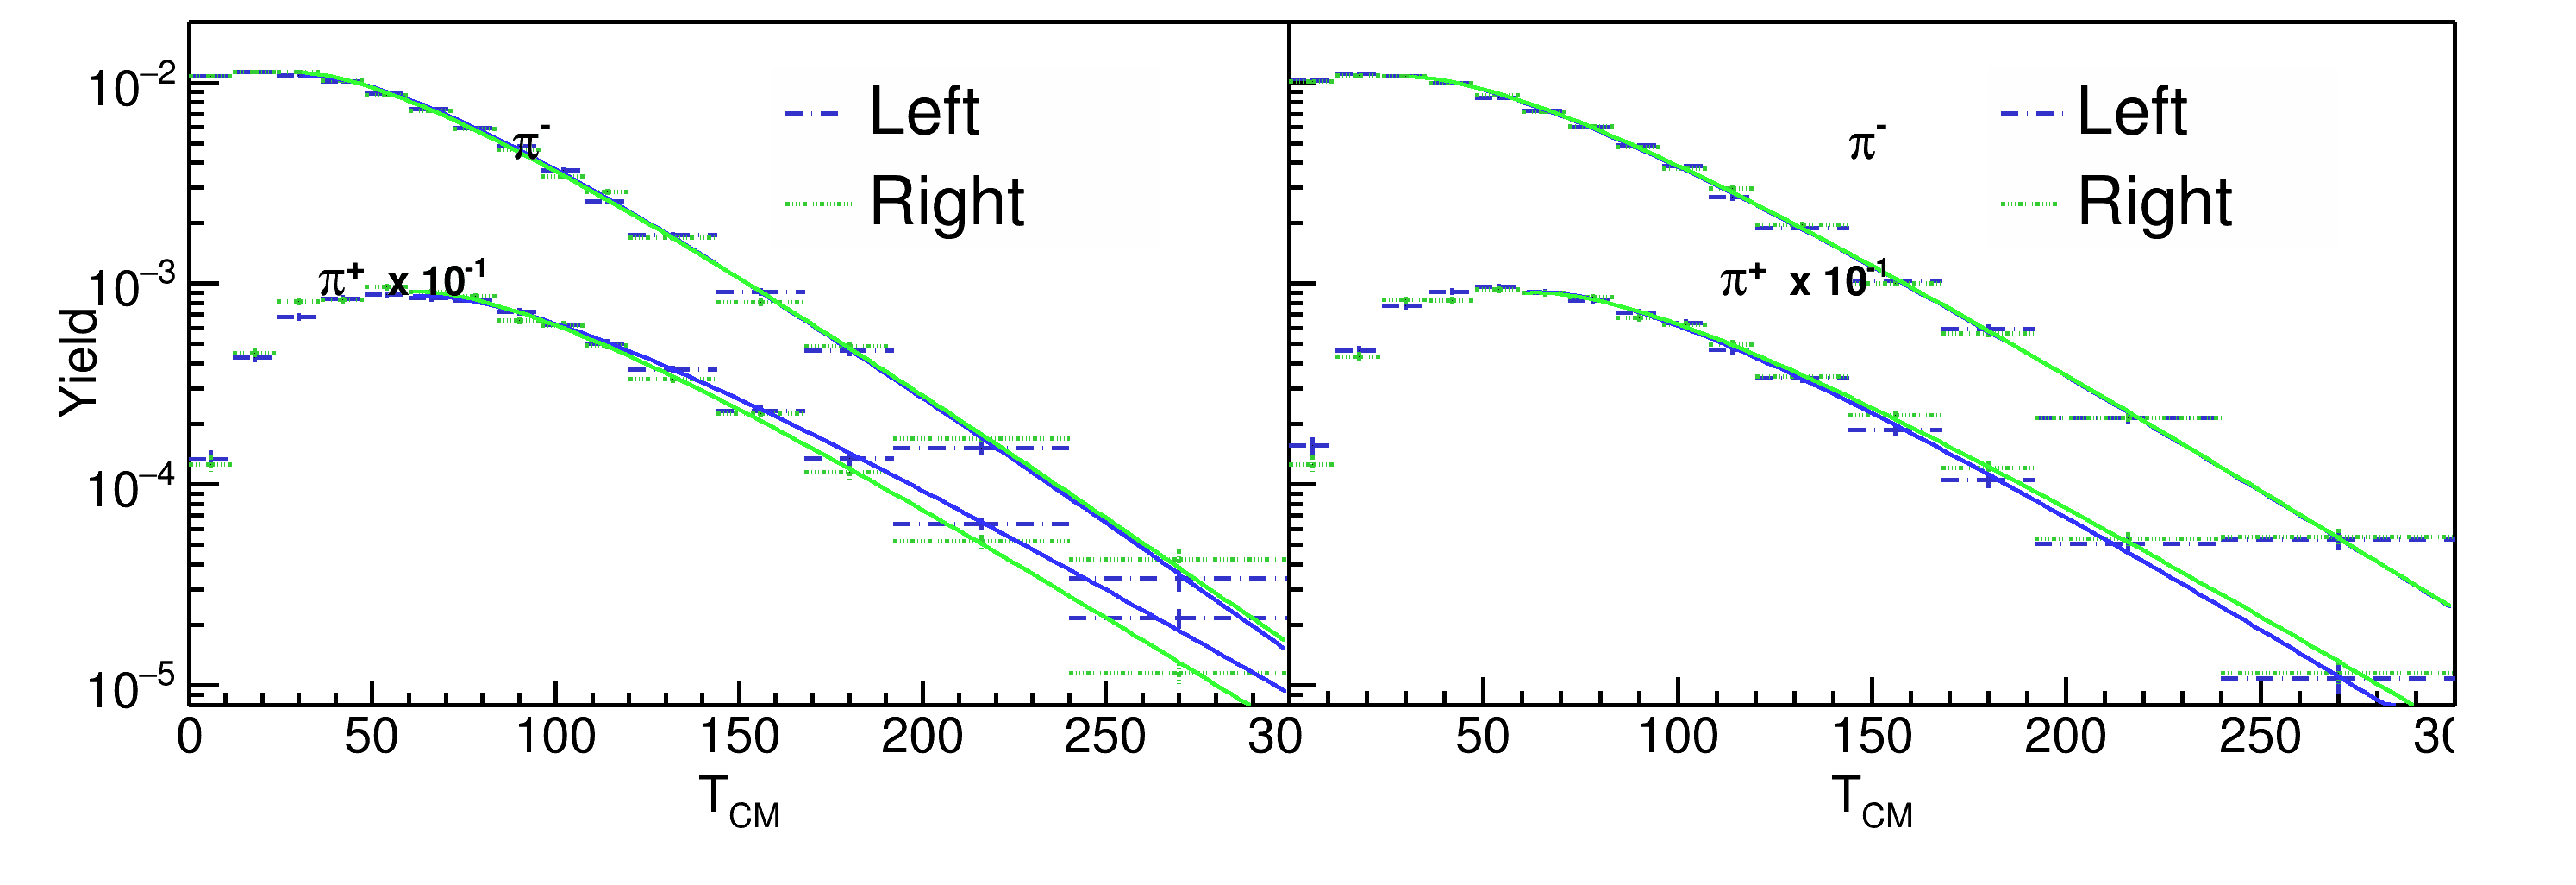
\includegraphics[width=\textwidth,valign=c]{sn132_SC} \label{fig:132momdist_sc}}}%
    \qquad
    \subfloat[$\tin{108}{112}$ system.]{{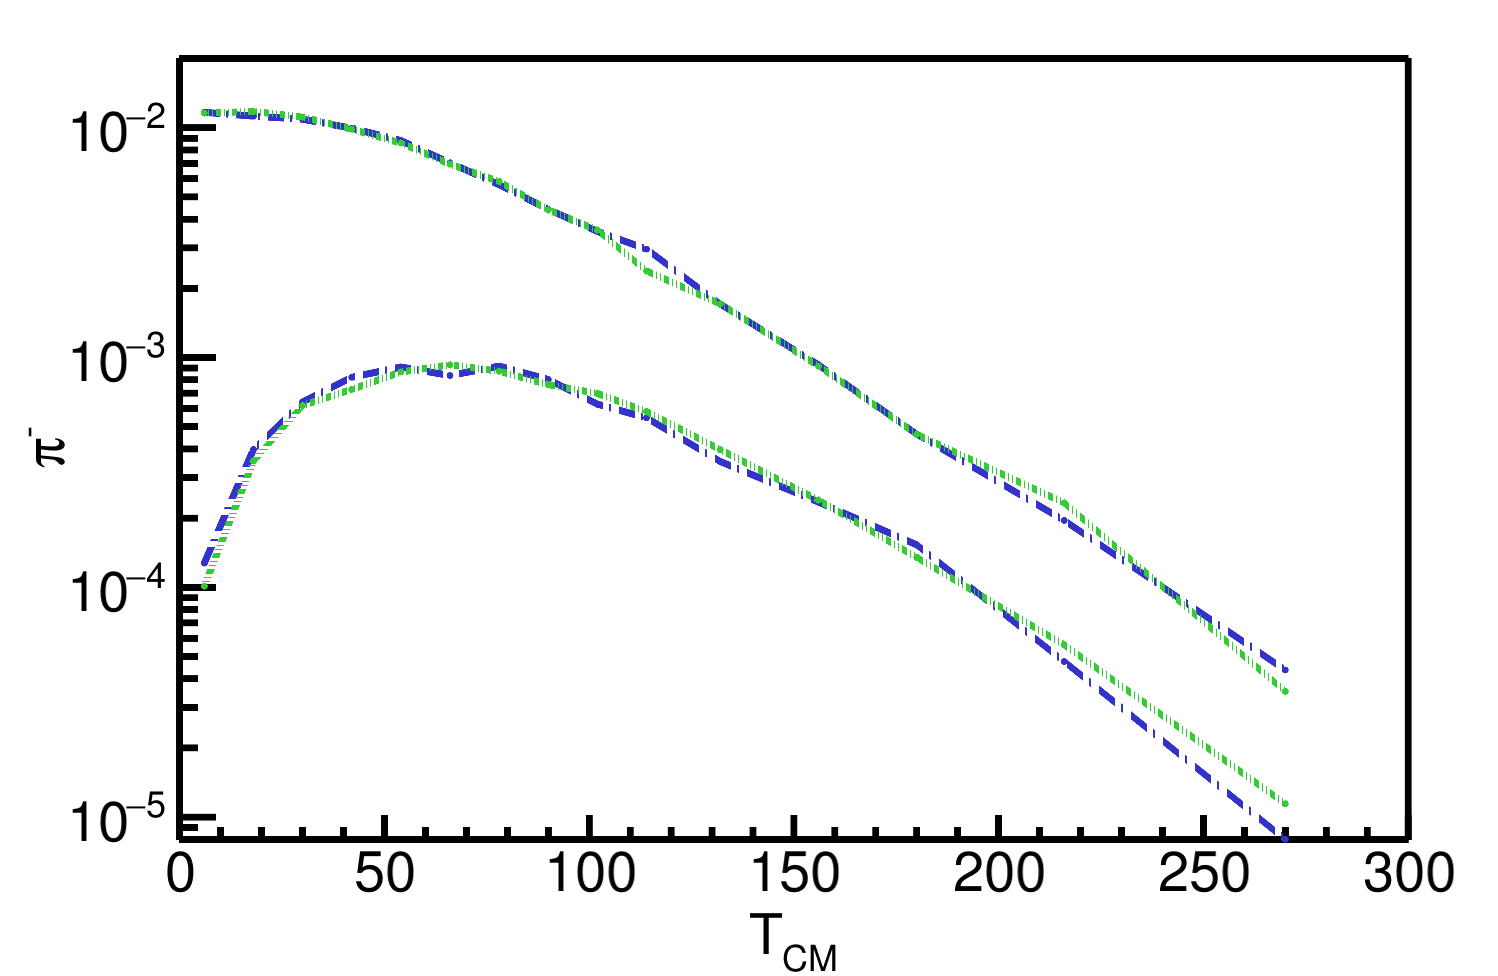
\includegraphics[width=\textwidth,valign=c]{sn108_SC} \label{fig:108momdist_sc}}}%
	\caption{Momentum distributions of the Left and Right sides of the TPC for $\pi^+$ and $\pi^-$ particles.}
	\label{fig:sc_momdist}
\end{figure}



This is one of the arguments for the success of the space charge correction task. Recall that only the relative distance between left and right-going tracks was minimized, and there was no guarantee that the corrected tracks coincide with the absolute BDC position at the target. The others being in agreement with the expected cocktail calibration beam as described in Section~\ref{sec:cocktail}.

Here we will discuss some of the final results of the pion kinetic energy spectrum as it pertains to the verification of the space charge analysis. The details of the pion PID analysis will be discussed in Section~\ref{sec:pid}. Figure~\ref{fig:sc_momdist} shows the $\pi^+$ and $\pi^-$ kinetic energy distributions in the center of mass system for the $\tin{132}{124}$ and $\tin{108}{112}$ systems. The momentum distributions are split into the beam-left and beam-right side of the TPC. For central collisions, one would expect no difference between the two momentum distributions due to the symmetry of the emission. As seen in the left panels of both figures, the data before the space charge correction is shown, whereas in the right panels the data after the space charge correction is shown. There is a significant improvement in the matching of the left and right side momentum distributions for both charged pion species, in both systems, especially for the high energy tail of the pions. It is remarkable that the DOCA observable provided a good enough measure of the average space charge in the chamber. There is no reason to assume correcting the DOCA distribution would correct the momentum distribution. This is the strongest evidence to the success of the space charge correction.



\section{CoBo timing correction}
The arrival time of signals originating from each pad may differ due to timing delays in the electronics and cabling. These timing differences affect the y-position measurement of each track. By measuring the y-direction track residuals, we find the timing differences correspond to about $\pm$\SI{2}{\milli\metre} in position differences. The timing difference is stable for each pad across several runs. 

\begin{figure}[!htb]%
    \centering
    \subfloat[]{{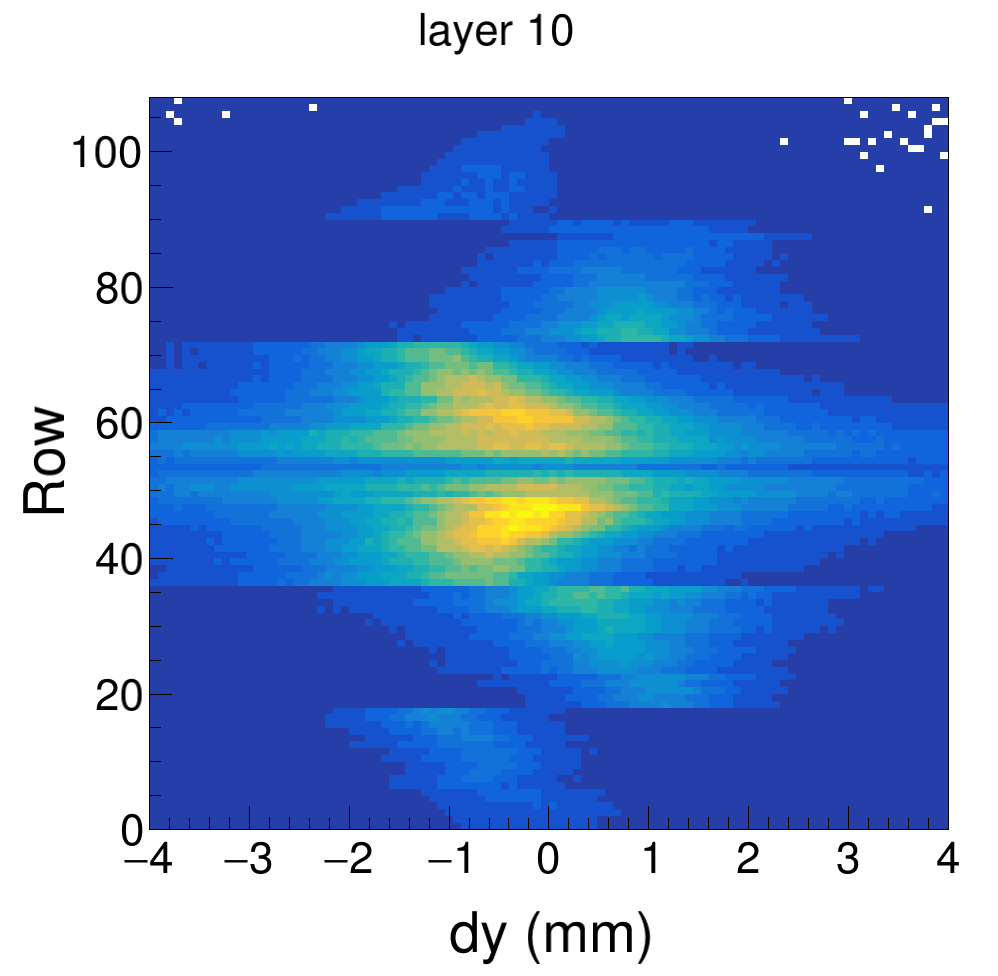
\includegraphics[width=.3\textwidth,valign=c]{run2907_yoffset6before_row_at_layer10.png} \label{}}}%
    \qquad
    \subfloat[]{{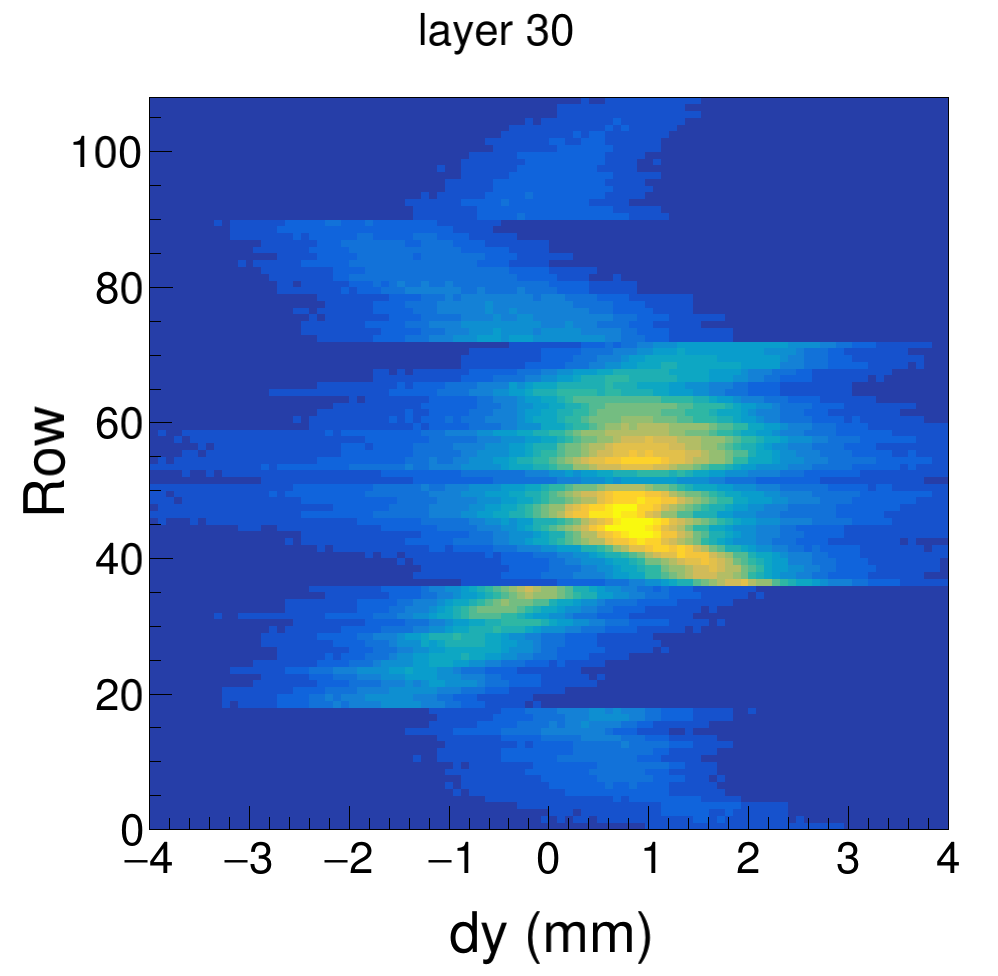
\includegraphics[width=.3\textwidth,valign=c]{run2907_yoffset5before_row_at_layer30.png} \label{}}}%
    \subfloat[]{{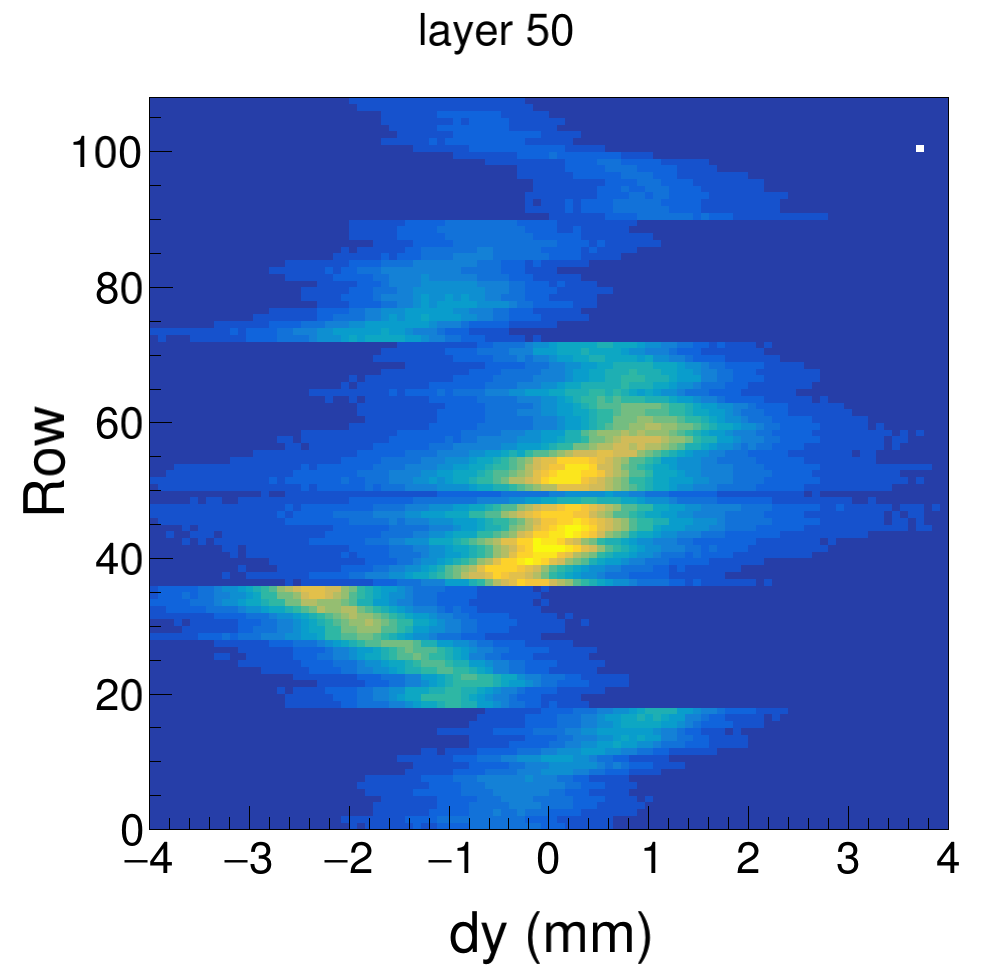
\includegraphics[width=.3\textwidth,valign=c]{run2907_yoffset4before_row_at_layer50.png} \label{}}}%\\
    
    \subfloat[]{{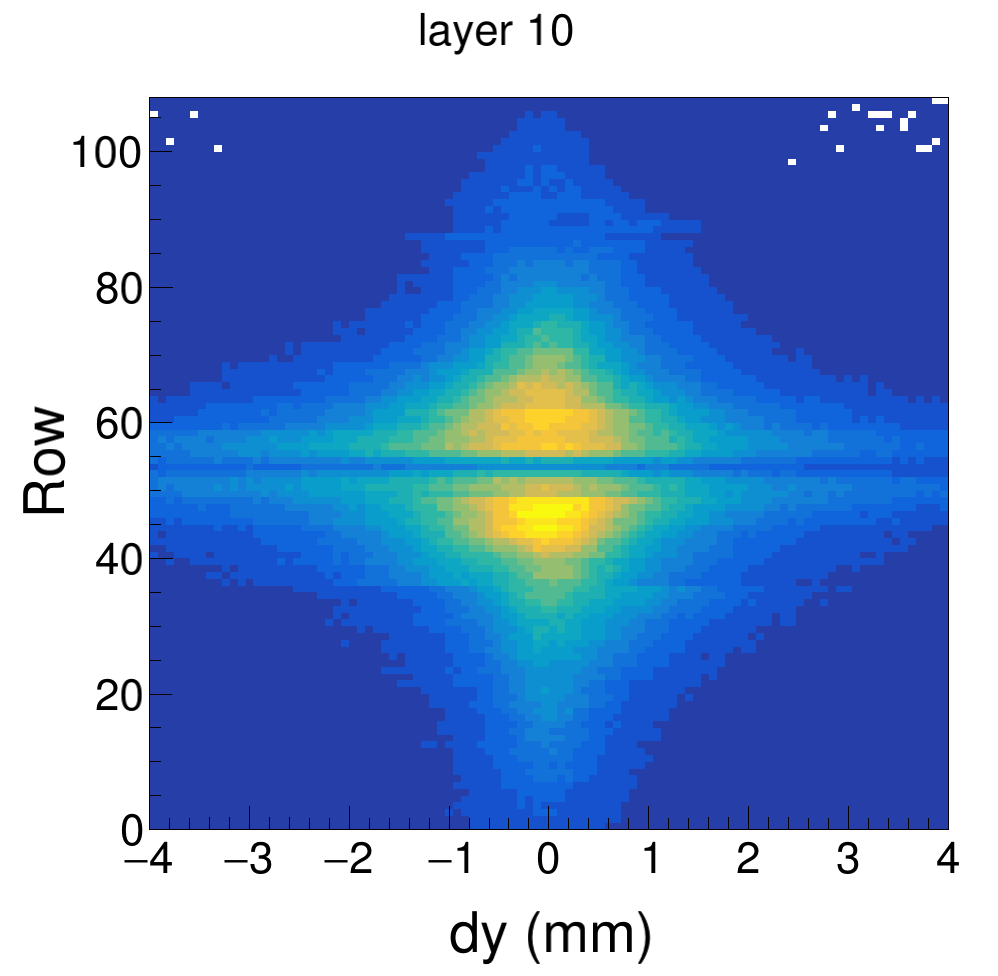
\includegraphics[width=.3\textwidth,valign=c]{run2907_yoffset6after_row_at_layer10.png} \label{}}}%
	\qquad
    \subfloat[]{{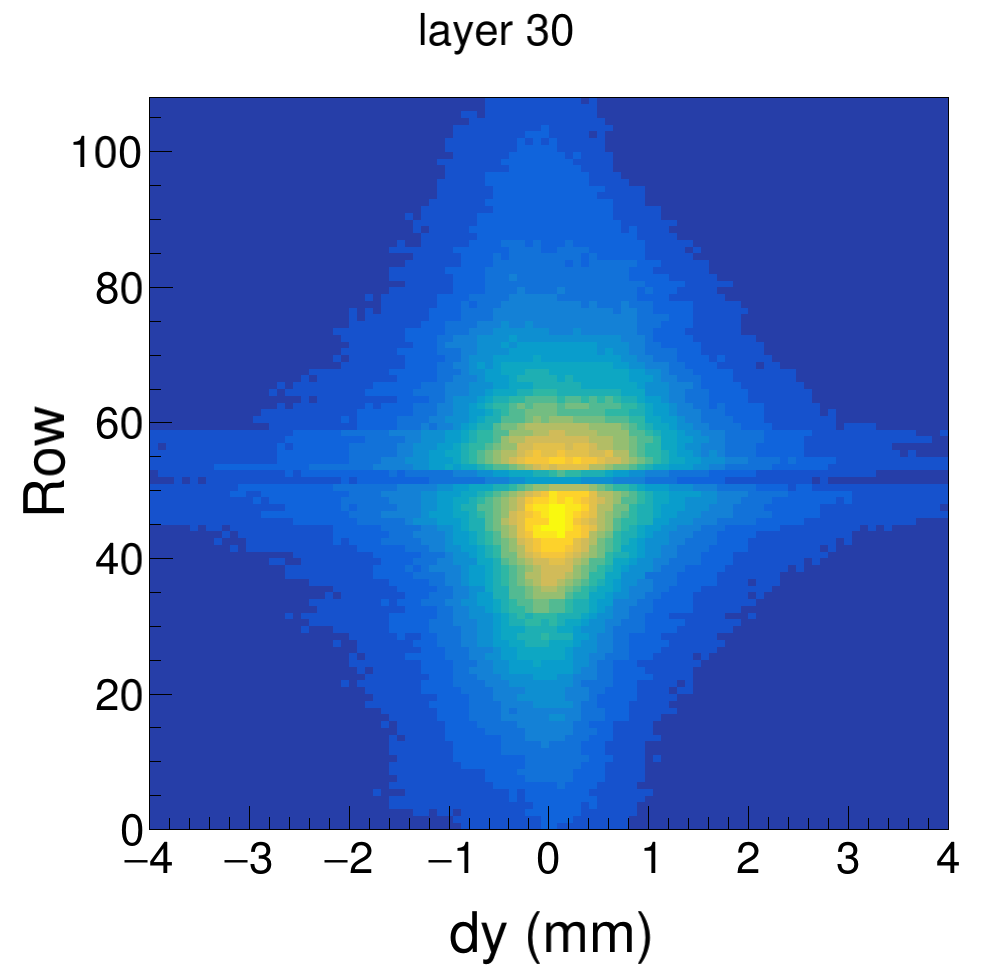
\includegraphics[width=.3\textwidth,valign=c]{run2907_yoffset5after_row_at_layer30.png} \label{}}}%
    \subfloat[]{{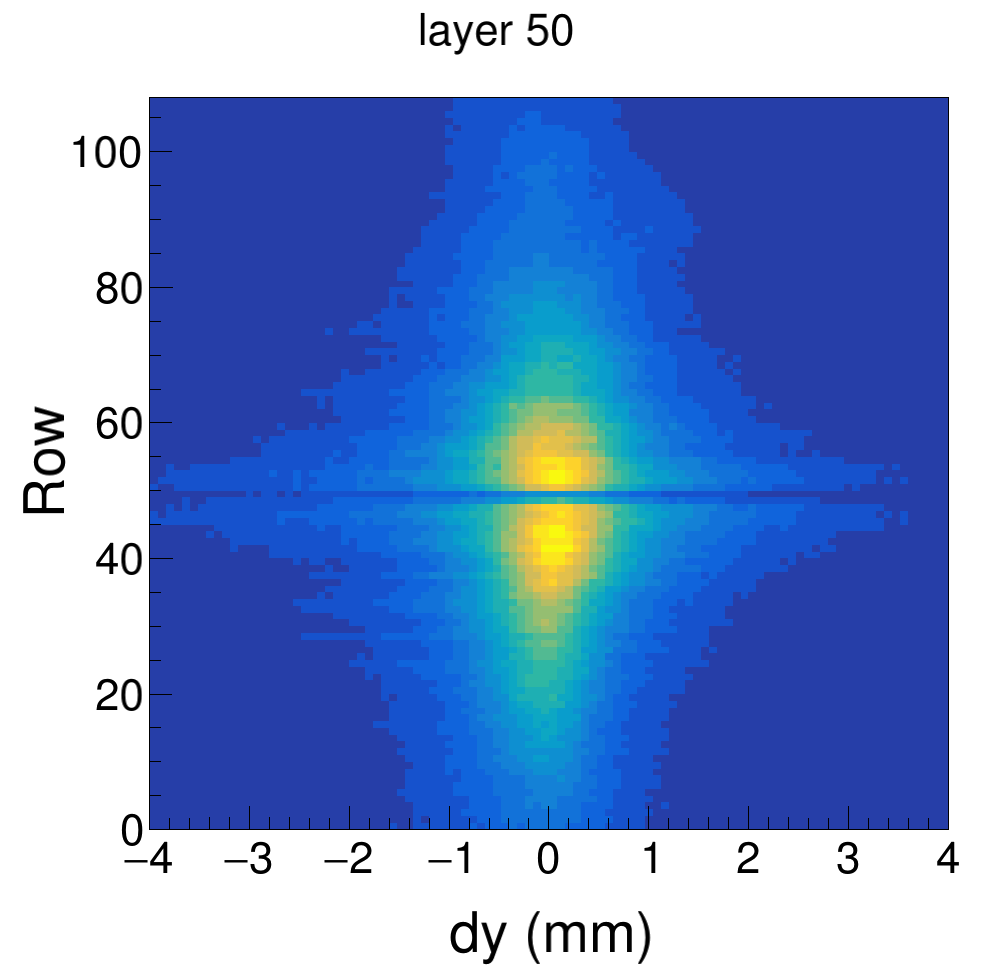
\includegraphics[width=.3\textwidth,valign=c]{run2907_yoffset4after_row_at_layer50.png} \label{}}}%

	\caption{Cobo timing correction for three different layers. One singe pad is represented by a unique layer and row number. The $dy$ residual of the track fitting shows, in the upper panel, that there is a timing calibration issue. This offset is fixed over several runs for a given pad. Therefore we can correct using a time correction map for each pad; the bottom panels show the distribution after correction. }
  	\label{fig:coboCorr}
\end{figure}



\begin{figure}[!htb]%
    \centering
    \subfloat[Before applying the timing correction.]{{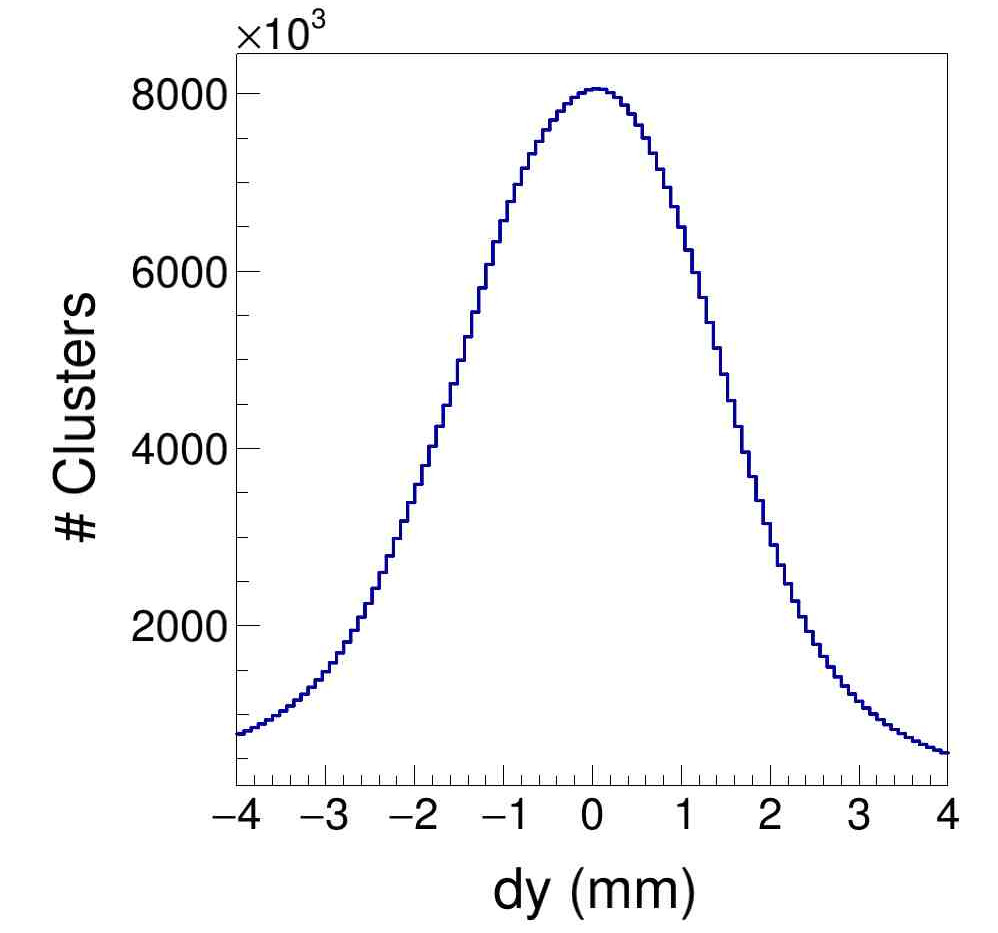
\includegraphics[width=.46\textwidth,valign=c]{run2905_yoffset1before_all.jpg} \label{fig:yoff_allBefore}}}%
    \qquad
    \subfloat[After applying the timing correction.]{{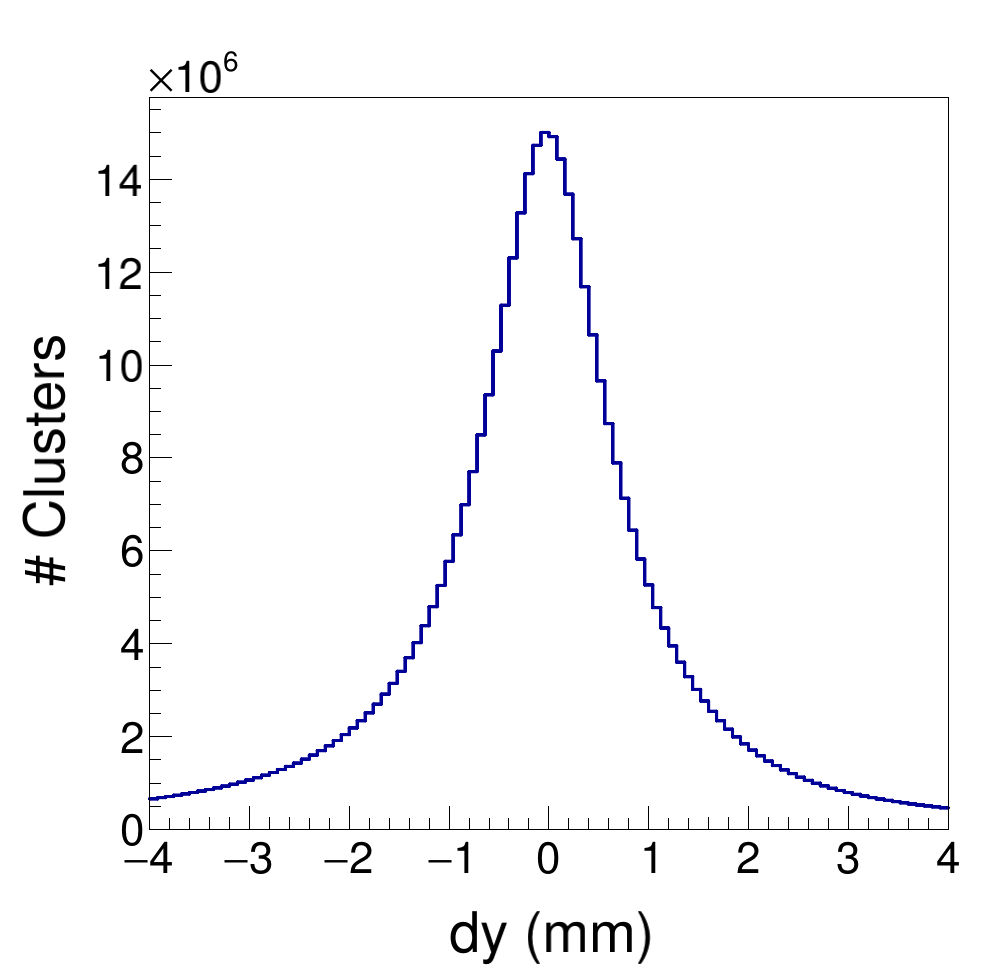
\includegraphics[width=.46\textwidth,valign=c]{run2905_yoffset1after_all.png} \label{fig:yoff_allAfter}}}%

    \caption{Y-residual distributions for all pads.}
	\label{fig:yoff}
\end{figure}


 Figure~\ref{fig:coboCorr} shows the y-residuals, across all the rows, for three different layers; where each row here represents a unique pad with a row and layer ID. Before the correction, one can see large deviations in the y-residuals which correspond to timing differences. The mean value of the y-residual distribution is fitted and an inverse correction map is constructed for each pad. The data is then reconstructed subtracting value from the inverse map, $dy$, for each pad. The resulting corrected distribution is shown in Fig.~\ref{fig:coboCorr} for the same layer set. Figure~\ref{fig:yoff} also shows the summary of all the pads before the correction and after the correction. There is a significant improvement in the width of the distribution going from \SI{1.5}{\milli\metre} to \SI{0.6}{\milli\metre}. 



%Reference appendix for poisson solver 
%Tables for ion drift velocity in P-10 Gas reference Sauli
%Figure of sDAC or POCA 
%Figure of cartoon of what is happening to tracks
%Figure of correction map in TPC and MC map 
%Figure of before and after correction BDC vs reco momentum
%Figure of track residuals before and after?



\section{Monte Carlo Simulation}
\label{sec:monteCarlo}

The MC simulation is composed of two separate simulations. The first simulation utilizes Geant4 to simulate the interactions of a particle passing through the various materials in the TPC. A scale model of the field cage was made, and the correct materials types were put in, with the correct gas mixture of P-10 gas at a pressure of 1 atm. The magnetic field map of the SAMURAI dipole magnet was also imported into Geant4 as well after assuming rotational symmetry along the axis perpendicular to the pole face -- since only 1/4 of the magnet was simulated. Along with the energy loss and particle transport, Geant4 also handles multiple scattering, and particle decays, which are all important effects especially for calculating the inefficiencies of pions. The output of Geant4 is a series of energy loss points which contain the amount of energy lost in $\si{\kilo\electronvolt\per\centi\metre}$ and the location of the energy loss in Cartesian space $(x,y,z)$. 

In the second part of the MC simulation, the physical processes of the TPC measurement are simulated, such as the electron drift, avalanche process, and all processes involved in the signal creation in the electronics. This is separated into three software tasks, the drift, pad response, and electronics tasks. In the following section we will discuss these tasks in more detail, the discussion of Geant4 is not covered here and the reader is refered to \cite{geant4}.  

\subsection{Drift Task}
 
 The first step of the drift task is to convert the primary and secondary ionization points of the MC track provided by Geant4 into electrons. The average number of electrons created in a gaseous detector,$N_{e^-}$, can be described as,
\begin{equation}
N_{e^{-}} =  \frac{\Delta E}{I},
\label{eq:kev2el}
\end{equation}
 
where $I$ is the ionization coefficient of P10 gas (Table~\ref{tb:gas}) and $\Delta E$ is the energy loss deposited. Each electron is then drifted along the electric field lines, under the assumption  that the electric field is uniform, which is true for most of the pad plane region. The total length drifted from the initial primary ionization point to the final anode wire is $L_{anode}$. 

\begin{table*}\centering
\ra{1.3}
\begin{tabular}{@{}rr@{}}\toprule 
\multicolumn{2}{c}{Electron Transport Gas Properties} \\
 \midrule
Drift velocity & 5.53 $\si{\centi\meter\per\micro\second}$\\
Transverse diffusion & 240 $\si{\micro \meter \centi\meter}^{-1/2}$\\
Longitudinal diffusion &  340 $\si{\micro \meter \centi\meter}^{-1/2}$\\
Gas Ionization & 26.2 $\si{\eV}$\\
\bottomrule
\end{tabular}
\caption{An overview of electron drift properties in P10 gas.}
\label{tb:gas}
\end{table*}

Drifting electrons frequently collide with the detector gas causing them to change direction. This stochastic motion is  described by a diffusion process occurring along the direction of travel (longitudinal) and transverse to the motion. The longitudinal ($c_{l}$) and transverse ($c_{t}$) diffusion coefficients are determined by Garfield++ calculation  \cite{garfield++} in the presence of a \SI{0.5}{\tesla} magnetic field, listed in Tb.~\ref{tb:gas}. The diffusion process is modeled by randomly sampling from a Gaussian distributions describing the diffusion in both of the directions. The random displacement vector is then added to the final position of the electron. The deviation in the transverse direction, $dr$, is randomly sampled from the distribution,

\begin{equation}
dr = e^{-\frac{r^2}{2\sigma_{t}^2}},
\end{equation}

where $\sigma_{t}=c_{t}\cdot\sqrt{L_{anode}}$.The transverse Cartesian directions can be written as $dx = dr \cdot \cos(\alpha)$ and $dz = dr \cdot \sin(\alpha)$, where $\alpha$ is a random angle from 0 to 2$\pi$, since there is no preferential angle  of emission in the transverse plane. The shift associated with the longitudinal diffusion, $dl$, is randomly sampled from, 

\begin{equation}
dl = e^{-\frac{t^2}{2\sigma_{l}^2}},
\end{equation}

where $\sigma_{l}=c_{l}\cdot\sqrt{L_{anode}}$. 

The final position of the electron along the wire is calculated  $x' = x + dx$. The electron will terminate on the closest anode wire, that is the anode wire that is closest to the shifted z-position $z\textprime = z + dz$, and the final electron z position is then updated to be the same as the anode wire it terminated on. The total drift time of the electron $t$ is calculated as,

\begin{equation}
 t = \frac{L_{anode} + dl}{v_d} + t_{offset},
 \label{eq:electronTime}
\end{equation}
 
where $v_d$ is the drift velocity. The parameter $t_{offset} = \SI{49.92}{\nano\second}$ is to allow for an alignment of the MC time bucket spectrum with the data. This is because the y-position corresponding to $t=0$ in the data time bucket spectra, does not correspond to the same position in the MC.  

Once the electrons have terminated on a particular wire, the avalanche process is simulated. The total number of electrons produced in the avalanche process of a single electron was simulated in Garfield++ and discussed in Section~\ref{sec:wireplanes} for the anode wire voltages used in the experiment. The number of electrons produced in the avalanche is randomly sampled from the Polya distribution  corresponding to the anode wire sections the electron terminated. The number of electrons produced is stored as a gain factor in that particular electron, instead of multiple instances of the original electron, to save storage space and computation time. 

%We assume that the lateral movement along the wire arising form $\vec{E}\times\vec{B}$ effect near the wire is negligible as compared with diffusion and other effects described later. 

It is worth mentioning there is the possibility to simulate the space charge effects in this task. This is not used for calculating the response of the TPC for efficiency calculations since it is a trivial exercise to input the space charge map only to then correct for it using the inverse map.  

\subsection{Pad Response Task}
The total charge of each avalanche is then distributed according to the pad response function (PRF) described in Section~\ref{sec:prf}. The PRF is simulated as the double integral of a 2-dimensional Gaussian. The final output charge on all the pads are the superposition of the PRFs of all drifted electrons. The MC PRF is expressed as, 

\begin{equation}
PRF(x,z) = \iint e^{-\frac{(x-x_o)^2}{2\sigma_x^2}} e^{-\frac{(z-z_o)^2}{2\sigma_z^2}}dxdz,
\end{equation}

where $\sigma_x = 3.4$ and $\sigma_z = 3.5$, and $x_0$ and $z_0$ are the final position of the drifted electron. These Gaussian parameters were determined as a best fit of the MC PRF and the experimental data PRF. 


\subsection{Electronics Task}

The purpose of the electronics task is to simulate the electronics response to a particular charge induced on each pad, converting charge into ADC channels. In a simplified picture, the induced charge on each pad goes through a pre-amplifier and shaping amplifier which determine the final pulse shape that is read out. The pulse shape did not change significantly in any circumstance, such as pulse height, data type, or particle type, as long as the electronics settings were fixed. This allows us to assume the pulse shape is constant and can be described by two variables, the height of the pulse, $Q$, and the starting time bucket of the pulse, $t_o$. The starting time of the pulse is defined as the time at 10\% pulse height, on the rising edge. The shape of the pulse depends on the shaping time constant which was set to \SI{117}{\nano\second} for the data analyzed here. Figure~\ref{fig:pulseshape} shows the pulse shape which was extracted from the experimental signals in the data. These were signals that did not saturate the electronics and were averaged over a wide range of ADC values. Here it is normalized so the maximum height is 1. 



\begin{figure}[!htb]
    \centering       
    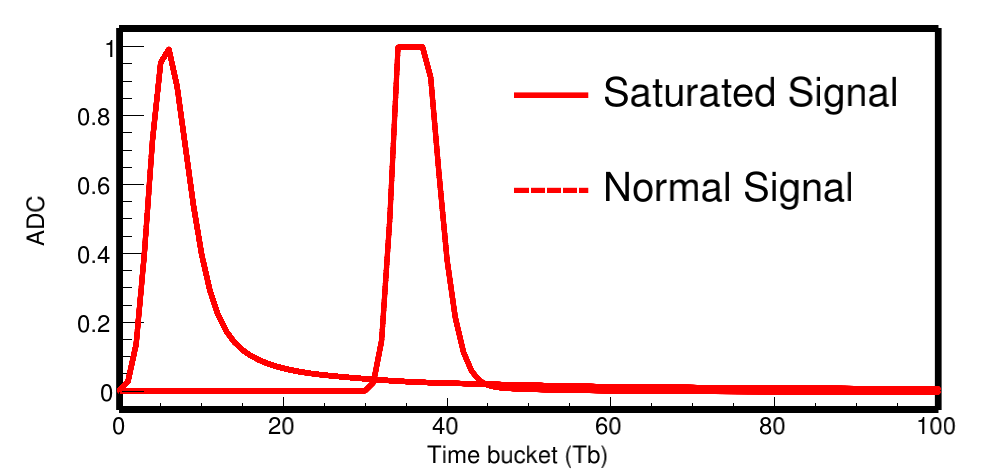
\includegraphics[width=\linewidth]{satpulse.png} 
    \caption{The standard pulse shape and saturated pulse shape extracted from the experimental data, and used in the MC software.}
    \label{fig:pulseshape}
\end{figure}


Converting the charge in each pad into the height of the ADC response in the electronics is calculated as, 

\begin{equation}
Q = f_G  N_{e}  \cdot e \cdot\frac{ADC_{max} - ADC_{pedestal}}{f_c}
\label{eq:etoADC}
\end{equation},

where $e$ is the fundamental charge of the electron in $\si{\femto \coulomb}$, $N_{e}$ is the total number of avalanche electrons, $ADC_{pedestal}$) is the pedestal (300 ADC, $\mathrm{ADC_{Max}}$ is the maximum allowed ADC value (4096), and $f_c$ is the dynamic range setting (\SI{120}{\femto\coulomb}). The pulse shape given in Fig.~\ref{fig:pulseshape} is multiplied by the pulse height $Q$ giving the full time bucket estimate of the TPC response. Random Gaussian noise is added to each time bucket, where the root-mean-squared value of the electronics noise was measured to be around 6 ADC. The timing information of the pulse is calculated from Eq.~\ref{eq:electronTime}. The coefficient $f_G$ corresponds to a factor which allows for fine tuning of the ADC calibration. This factor is calculated by

\begin{equation}
f_G^p = \frac{\langle dE/dx\rangle_{Data}^p}{\langle dE/dx\rangle_{MC}^p}
\label{eq:dedxcalibration}
\end{equation}

where $\langle dE/dx\rangle_{MC}^p$ and $\langle dE/dx\rangle_{Data}^p$  are the energy loss values for a particle in a given momentum bin $p$. The calibration will be discussed later in Section~\ref{sec:mccomparison}.


\section{Monte Carlo Track Embedding}
\label{sec:embedding}

There are several effects in a complex experimental setup that influence the data in either unknown or un-quantifiable ways. One such effect is the bias of the triggering system, here the Kyoto and Katana multiplicity arrays preferentially select data that are emitted in a particular reaction plane. As previously discussed, the saturation effects of the electronics, notably the shadowing of other tracks. The effects of track multiplicity and the distribution of heavy ion and residues from the breakup of the target and projectile which can cause tracking failures. In these cases, a full MC simulation would be cumbersome if not impossible to do. Simply put, there is no better substitute for simulating experimental data, than the experimental data itself. By embedding MC tracks into experimental data -- and propagating through the tracking and reconstruction algorithm -- one can account for all these sources of biases which are contained in the data, while at the same time measuring the response of the TPC.

%As discussed in Section~\ref{sec:software}, the software is composed of several tasks, each of which have the possibility of introducing errors or biases through assumptions made in the tracking algorithm. The TPC system itself introduces errors related to the physical measurement which can be addressed through modeling the TPC, and its materials. 

%For all of the sources of biases in the TPC, it is clear that a MC type approach to solving for the response of the TPC would be the most practical method. Also by embedding MC events into real data we can take into account the effects of the experimental setup as well as the software and the detector system all together at once. Track embedding is the process of taking a MC simulated track and embedding its response into an experimental data event. After reconstructing this new embedded event we match the input MC track to the corresponding final reconstructed track.  By doing so, we can evaluate the response of the entire TPC system to any given input. 



%\begin{sidewaysfigure}[!htb]
%\centering
%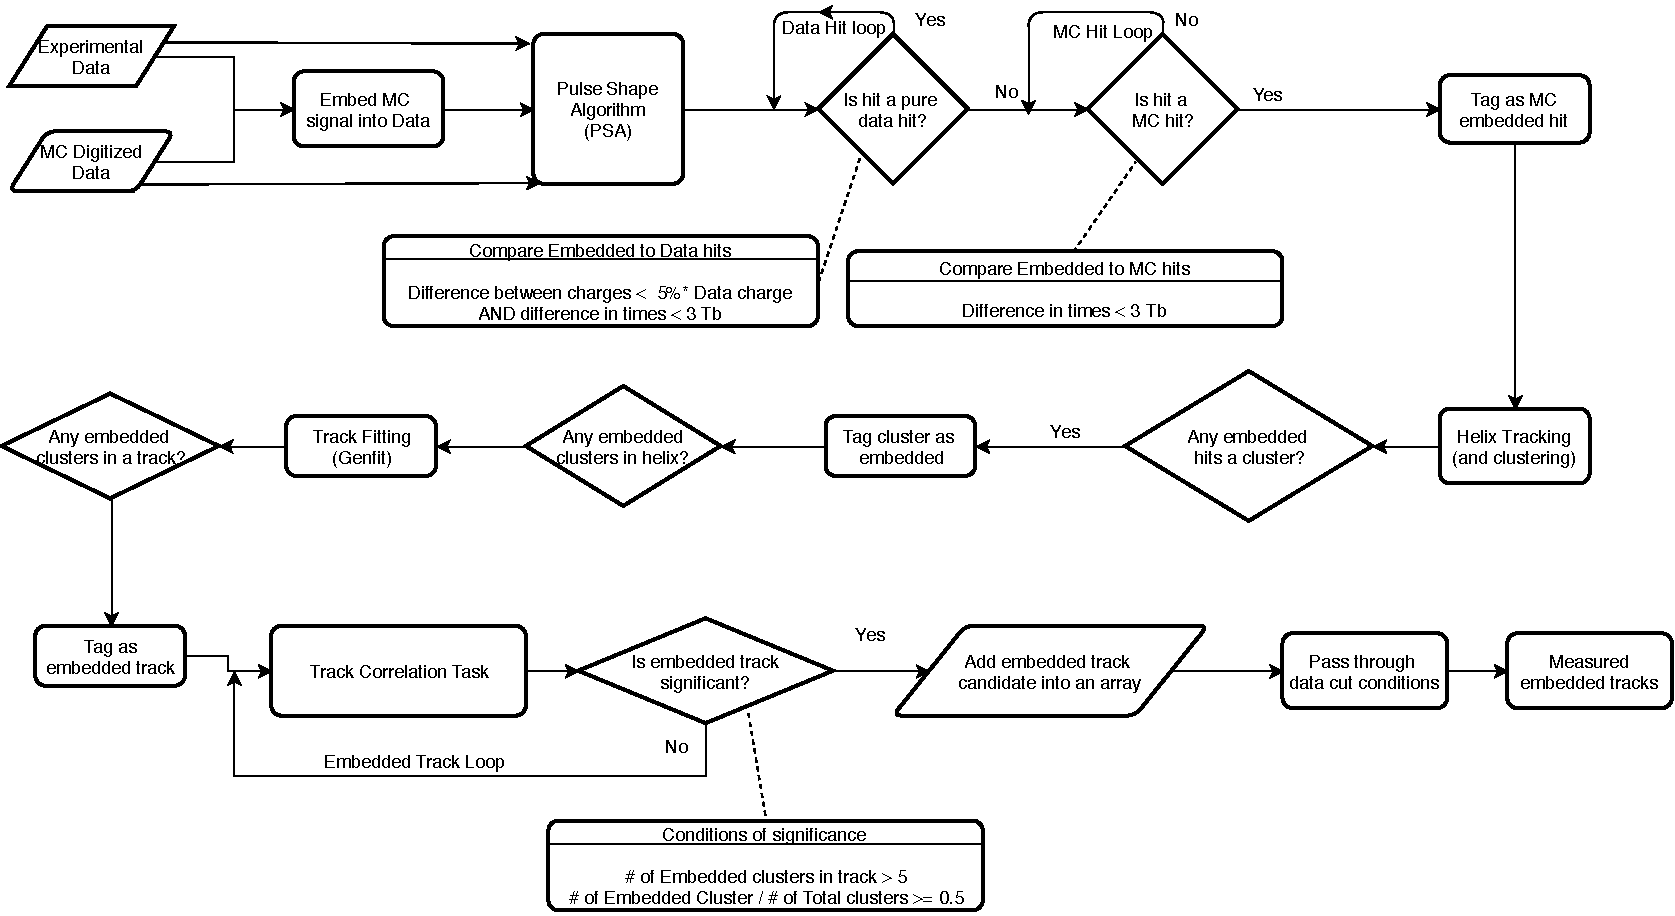
\includegraphics[width=\textwidth]{FlowEmbedding.pdf}
%\caption{Flow of embedding implementation in the software.}
%\label{fig:flow}
%\end{sidewaysfigure}


%\clearpage
%\pagestyle{lscape} % first clear the page and change the pagestyle
%\begin{landscape}
% your landscape table(s) or figure(s) here
%CONSIDER ROTATING THIS FIGURE IF ALLOWED
\begin{figure}[!htb]
\centering
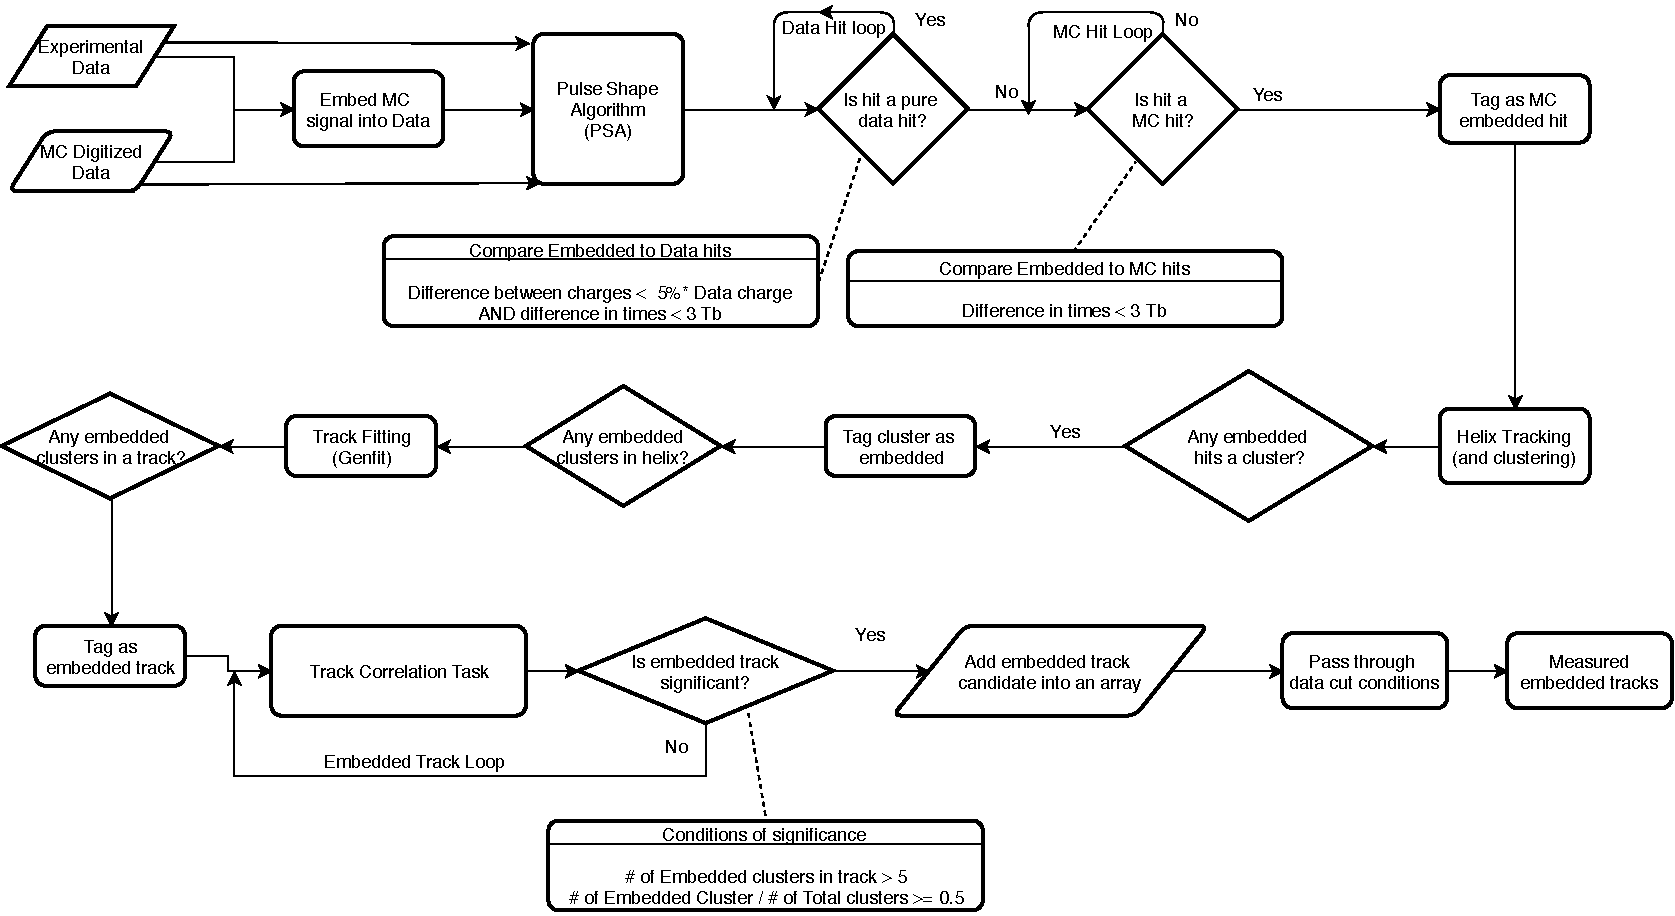
\includegraphics[width=\textwidth]{FlowEmbedding.pdf}
\caption{Flow diagram of the embedding software.}
\label{fig:flow}
\end{figure}

%\end{landscape}
%\pagestyle{plain}

\begin{figure}[!htb]%
    \centering
    \subfloat[200 MeV/c $\pi^-$ MC digitized track]{{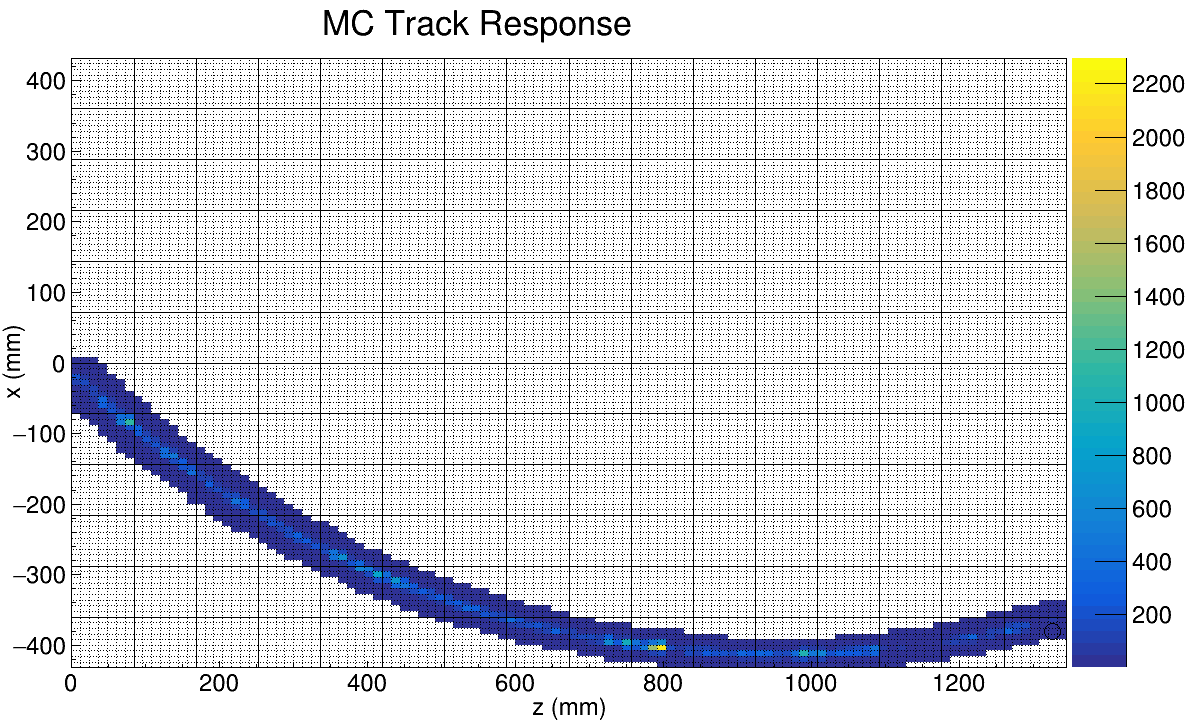
\includegraphics[width=.46\textwidth,valign=c]{mcresponse.png} \label{fig:mcevent}}}%
    \qquad
    \subfloat[Experimental data event.]{{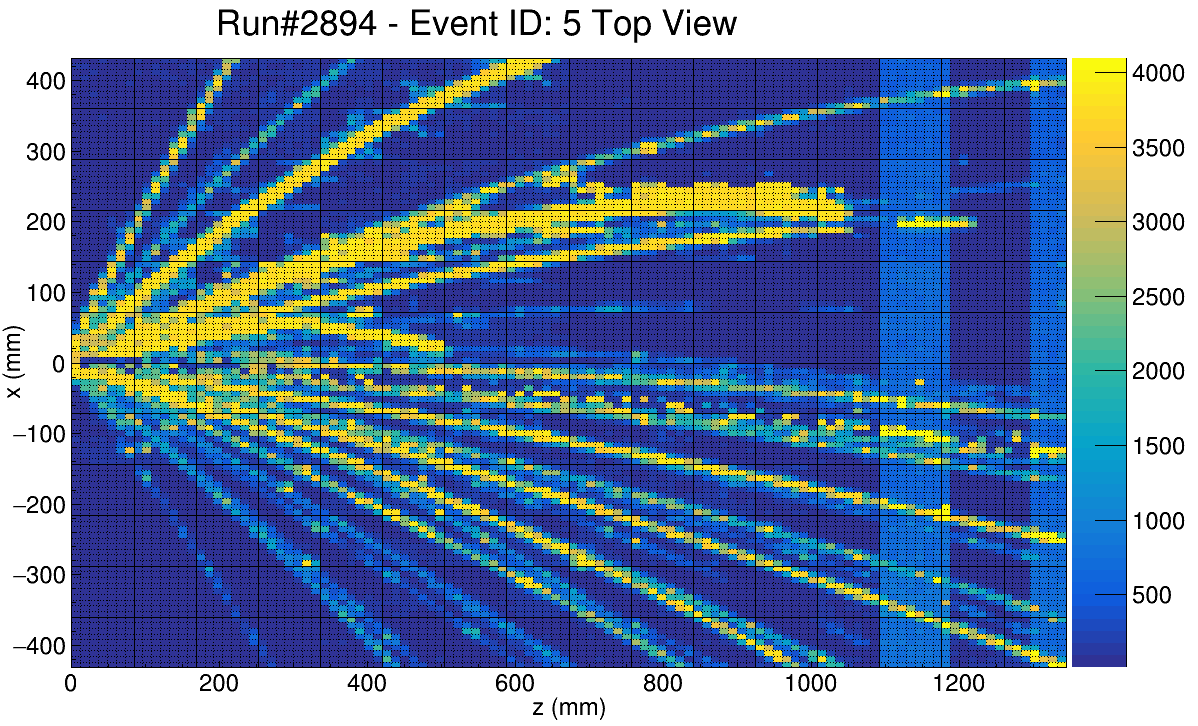
\includegraphics[width=.46\textwidth,valign=c]{event5.png} \label{fig:dataevent}}}%
    \caption{Charge readout of the pad plane, showing the max ADC in a given pad, for both the MC simulation and experimental data.}
	\label{fig:mcDataEmbedtrack}
\end{figure}


\begin{figure}[!htb]%
    \centering
    \subfloat[Perspective view.]{{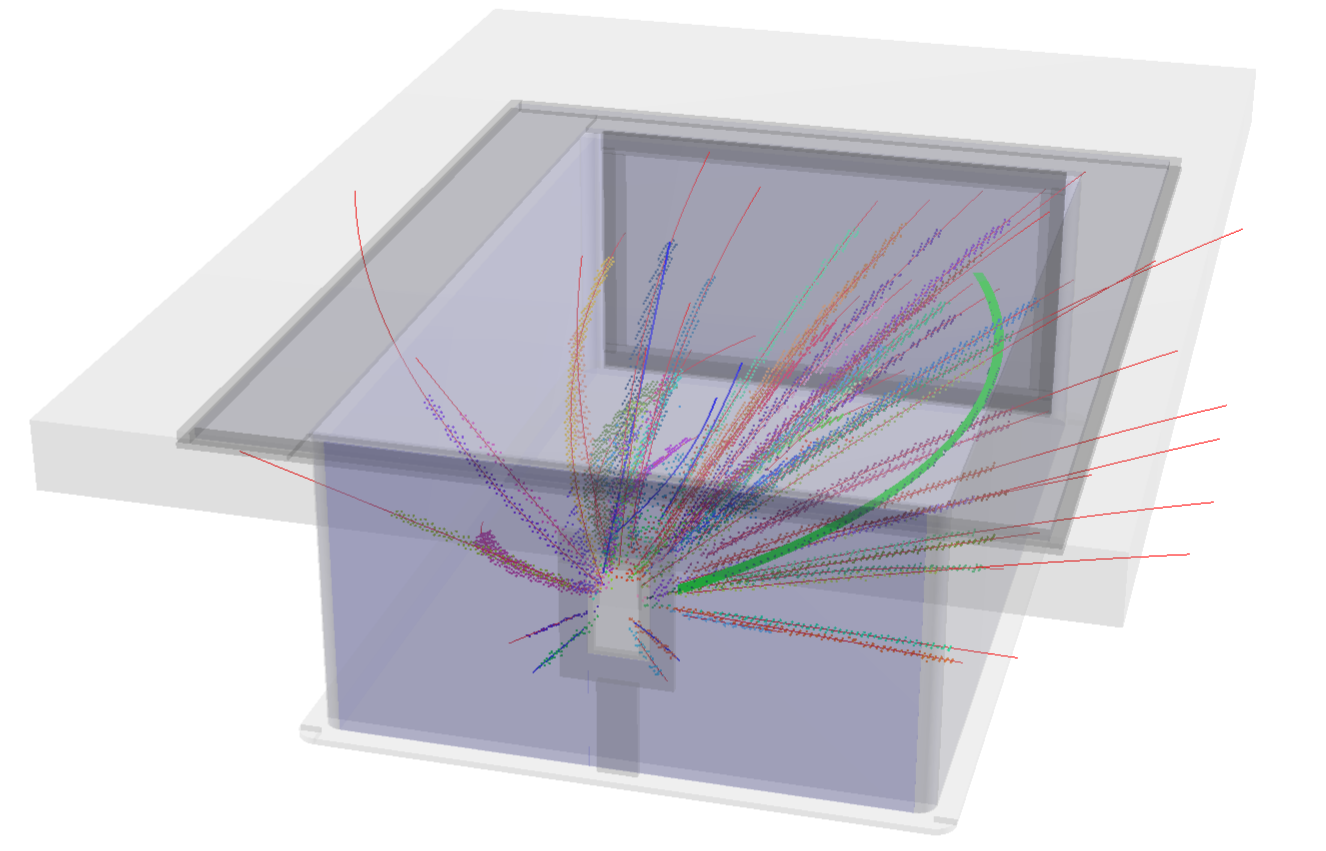
\includegraphics[width=.5\textwidth,valign=c]{perspective_embed} \label{fig:persEmbed}}}%
    \qquad
    \subfloat[Top down view.]{{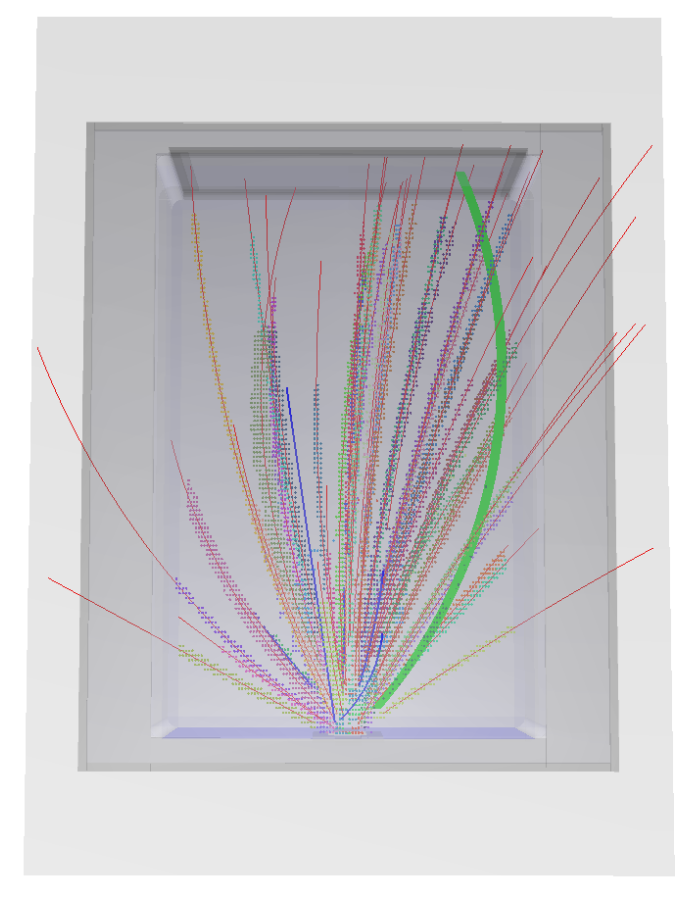
\includegraphics[width=.3\textwidth,valign=c]{top_embed} \label{fig:topEmbed}}}%
    \subfloat[Side view.]{{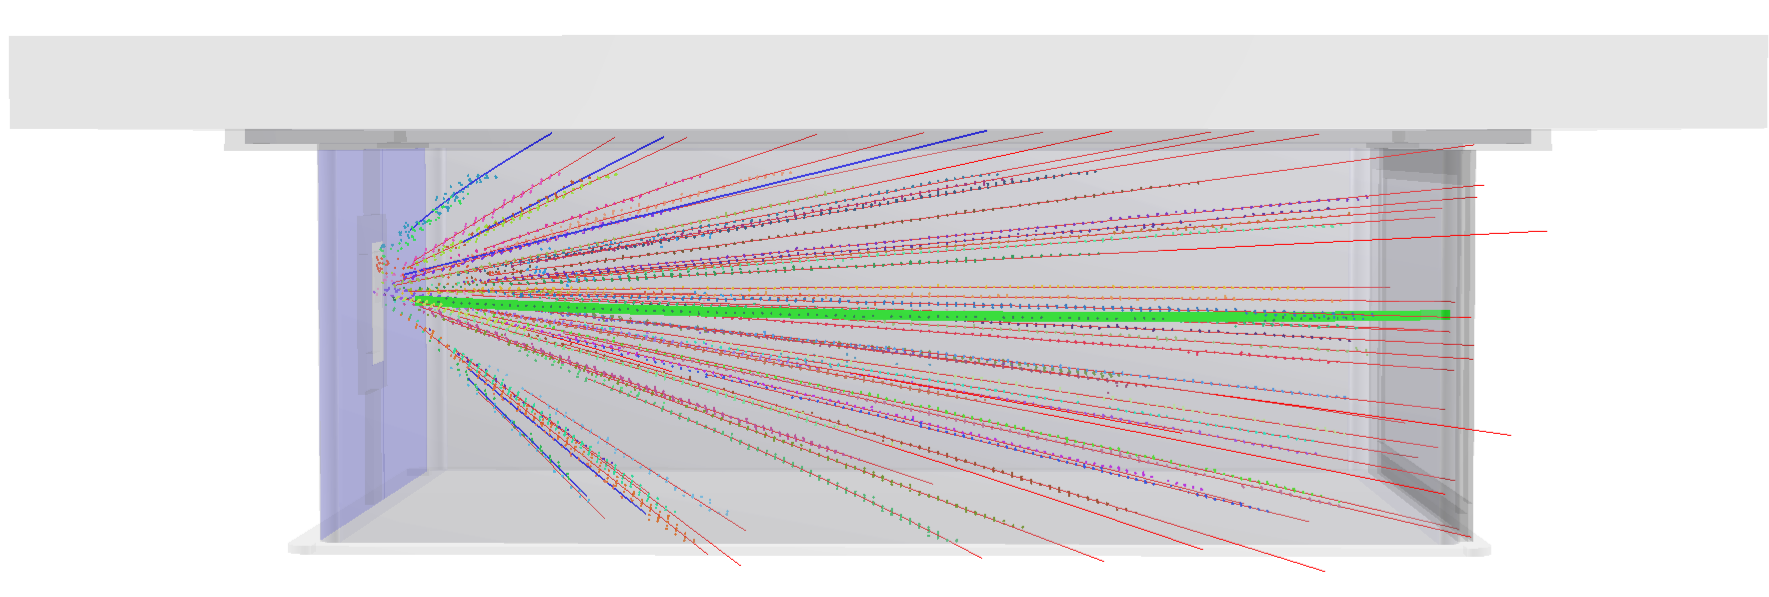
\includegraphics[width=.55\textwidth,valign=c]{side_embed} \label{fig:sideEmbed}}}%
  
    \caption{A 200 MeV/c $\pi^-$ embedded into a nuclear collision type event. The embedded track identified by the software is highlighted by the solid green line. }
	\label{fig:embedtrack}
\end{figure}


The detailed software flow diagram of the embedding algorithm is shown in Figure~\ref{fig:flow}. Starting from Geant4 and passing through the 3 MC digitization tasks described above, the output response of the MC track in the TPC is created. From here we directly embed the MC signals into experimental data by adding the MC signals directly into the experimental time bucket spectrum, pad-by-pad. As will be described in Sec.~\ref{sec:simSat}, prior to embedding the MC signals, all pads which are saturated in the experimental data are identified and flagged. MC signals are forbidden to be embedded after the (MC) saturation time bucket position identified in the procedure outlined in Section~\ref{sec:simSat}. Figure~\ref{fig:mcevent} shows the response of a \SI{200}{\mega\electronvolt\per\clight} $\pi^-$ track in the TPC. Figure~\ref{fig:dataevent} shows this track embedded into an experimental event. In the following, here I will refer to experimental data with embedded MC signals as \emph{embedded data} for short, the MC generated response as \emph{MC data}, and data only containing the experimental signals as \emph{experimental data}. The three sets of data are independently analyzed by the PSA algorithm described in Section~\ref{sec:psa},  which finds all the hits associated with each data set. These three independent hit data sets are temporarily stored. 

Here within the PSA algorithm, is the first and most important part of the embedding software. If the embedding portion of the PSA task is turned on,  it has the job to identify which hits in the embedded data set originate from the MC hits set and which are from the experimental data. Once the MC hits are identified, these embedded hits can be tagged and tracked through the entire software. 

First, the hits in the embedded set are matched against the experimental data, identifying which of the embedded hits originate from the experimental hit set. For two hits to match, they must satisfy two criteria, $\left|(Q_{\mathrm{Data}} - Q_{\mathrm{Embed} })/Q_{\mathrm{Data}}\right| < .05$ and $\left|t_{\mathrm{Embed} } - t_{\mathrm{Data} }\right| < 3$ where $Q$ and $t$ represent the charge and time of the hit respectively. Hits that satisfy these criteria are then removed from the embedded data set.

The surviving hits are then compared with the MC hit data set, where the criteria for a matching MC hit is, $\left|t_{\mathrm{Embed} } - t_{\mathrm{MC} }\right| < 3$.  There is no requirement for a matching criteria for the charge values which would artificially bias the charge values selected depending on our cut. This is critical for minimum ionizing particles such as pions; this can only be accomplished by first removing almost all of the experimental hits as was done in the first step. Each embedded hit that passes this step of criteria is tagged as originating from a MC hit. From here, the embedded data is treated as if it were real data passing through the same software analysis. 

 If a helix track has one hit that is embedded it will also be tagged as embedded. When the hits in a helix track are clustered, if a cluster contains one embedded hit it is itself tagged as an embedded cluster. Furthermore, if a track that is reconstructed contains any embedded clusters, it is tagged as an embedded track also. The goal of this na\"ive tagging approach is to preserve all the information of where the embedded hits, clusters, and tracks have gone, preserving as much information until the end without introducing a bias.
 
  When MC embedding is performed, another task is added to the end of the analysis routine, namely the embedded correlation task. It is the job of this task to identify which of the final embedded tracks are candidates for the original input track. For example, several things may happen along the process of embedding that may disqualify a track as a candidate in this na\"ive tagging approach. A track could break up, lose or share its charge with an adjacent track, or it may not be identified at all for a variety of other reasons. For the final reconstructed track to be a candidate for the input MC track, it must satisfy two conditions, $N_{sat} > 5$ and $N_{\mathrm{sat}}/N_{\mathrm{Total}} \geq .5$, where $N_{\mathrm{sat}}$ is the number of saturated clusters in a track, and $N_{\mathrm{Total}}$ is the number of total clusters. The first criteria is a simple minimum cut where to ensure the minimum condition of a embedded track is met at least having 5 clusters. The second criteria is the strongest cut, ensuring the track has at least half of its clusters coming from embedded MC signals. The set of tracks which satisfy both conditions are saved into an array of candidate tracks, which may represent the original MC track. This is done so that if any track splitting has occurred, all of the split tracks will be saved into the vector. it is then left to the user to decide how to further study these tracks. 

If the embedded track is split into multiple tracks, the user must select what they believe to be the track which most represents the original track, for the purposes of calculating efficiency. This is to preserve the definition of efficiency is strictly $\leq 1$. Typically only one of the tracks in the set will satisfy one of the reasonable quality cut conditions in an analysis which will be discussed further in Section~\ref{sec:qualitycut}. For example, the most reasonable assumption is the track originating from the vertex is the most correct in this case, whereas the split fraction of the track wont originate from the vertex but instead have a large distance to vertex value. In this thesis, the track with the minimum distance to vertex is identified as the track in which the efficiency analysis will be performed.



\subsection{Simulating Saturation}
\label{sec:simSat}

Since saturation is one of the largest and most important effects in the data, simulating it correctly in MC embedding becomes paramount. In general all preamplifiers have a finite range of output values set by a positive and negative rail (typically -12V and +12V). If the input charge into a charge sensitive preamplifier causes the output voltage to reach the max (or min) output voltage, the preamplifier saturates and the response may be non-linear. The picture is complicated by the fact that there is usually an RC feedback loop which dissipates the input charge. The time a pre-amplifier returns to linear behavior depends on the input charge and how quickly it can be dissipated \cite{akiGET}. The pad is otherwise considered dead and no further charge can be measured until the channel can recover. There are several types of saturation that must be simulated or accounted for to correctly model the TPC response. They all are varying degrees of the same effect which manifest in different ways in the detector. 
 
Due to the long, high energy tail in  the energy loss distribution of a particle traversing matter, it is common to see pads along the track which have collected large energy loss values saturating the electronics of a couple of pads. This occurs for all tracks, even for minimum ionizing tracks. In this case, the saturation is infrequent and typically not an issue as there are many other clusters that are not saturated. As the charge of the particle gets higher, or the momentum gets lower, the  energy loss value also becomes higher, and a significant fraction of pads in a track may be saturated. In Section~\ref{sec:desat}, we outlined an algorithm to correct for the saturation for a  particular track, but saturation also affects the measurement of surrounding tracks. In order to make an accurate MC simulation, we must understand how saturation affects surrounding tracks. 

Pads that saturate have no signal or are \emph{dead} for a given amount of time after the saturating signal, depending on the input charge. For charges that are at or above the level of the dynamic range, the pad will certainly be dead from that moment on for the remaining time of the measurement. Signals from tracks passing directly underneath this pad, arriving later in time,  will therefore not be observed in that pad. In a sense the saturating signal is \emph{shadowing} any future tracks. As the track multiplicity of an event increases, the probability of track shadowing increases. This will change event by event and is very difficult to simulate except through a MC track embedding approach, which will be discussed in Section~\ref{sec:embedding}. 

\begin{figure}[!htb]
\centering
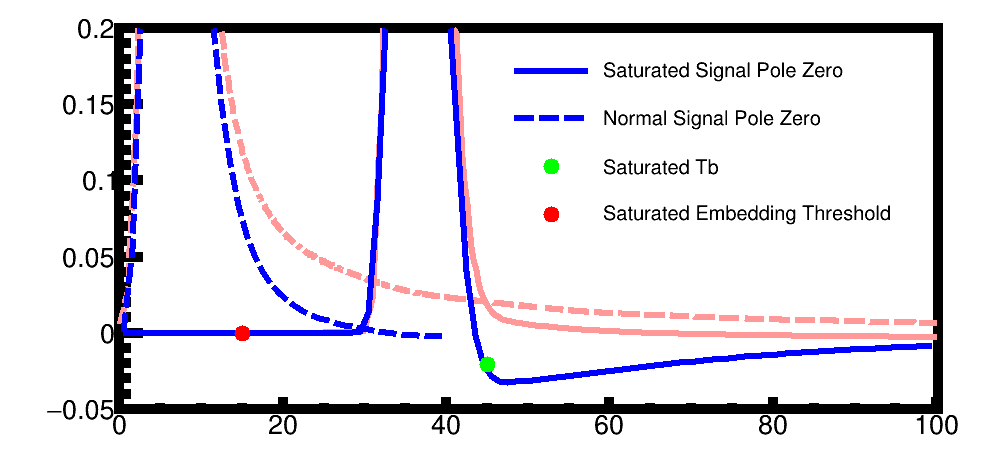
\includegraphics[width=\linewidth]{satpulsepz.png} 
\caption{Example of the pole zero correction when applied to the normal pulse and saturated pulse.} 
\label{fig:pulseSatTag}
\end{figure}


When the input signal is very large, the electronics can be dead for up to \SI{35}{\milli\second} \cite{akiGET}. The beam rate in the experiment was about \SI{10}{\kilo\hertz}, which corresponds to an average of \SI{100}{\micro\second} between subsequent beams. In this case, channels can be effectively dead for several events before recovering. There is a large amount of high energy electrons, commonly referred to as \emph{delta rays},  which are produced from the beam passing through the gas. The number of electrons produced scale with the charge of a particle, in which the Sn beam produces several high energy electrons \cite{pdg}. In the presence of the magnetic field, almost all of the electrons traveling perpendicular to the field curl up and cannot travel very far, even for very high energy electrons. Figure~\ref{fig:deltaE} shows the horizontal and vertical extent of the delta rays in a top down and side views of the TPC. While many electrons can stop in the gas, some electrons have a high enough kinetic energy in the vertical direction where they can penetrate the gating grid without being blocked. Then they either terminate on the anode wire or possibly deposit their charge directly in the pad. In either case, the charge induced on the pad is large enough to kill the pad for a time long enough to last until at least the next event. This manifests as random dead pads in the experiment, that follow the beam path.  

%Example picture of dead pads?


\begin{figure}[!htb]%
    \centering
    \subfloat[Top view]{{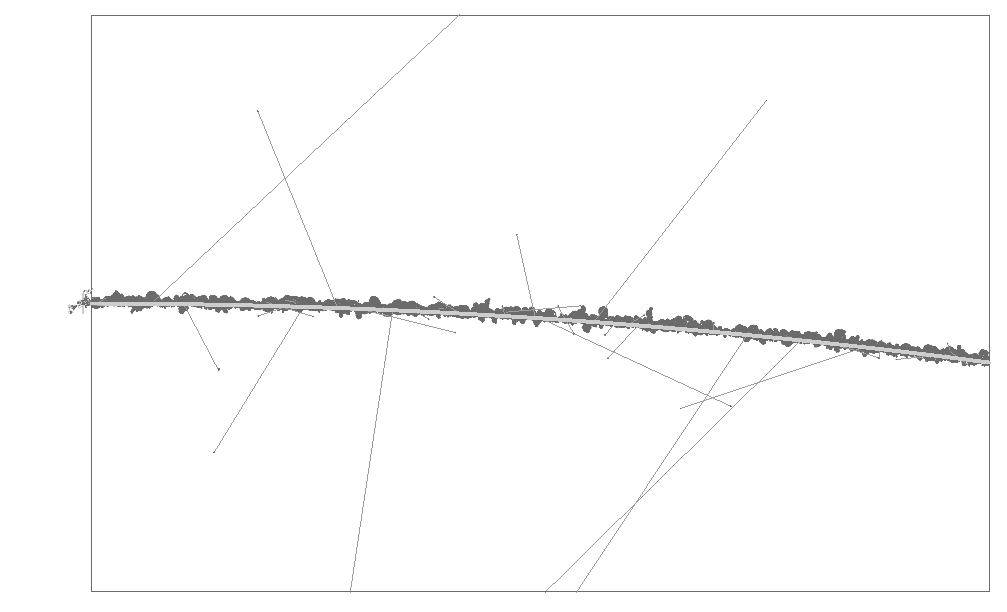
\includegraphics[width=.46\textwidth,valign=c]{deltaE_topview_neg} \label{fig:deltaE_topview}}}%
    \qquad
    \subfloat[Side view]{{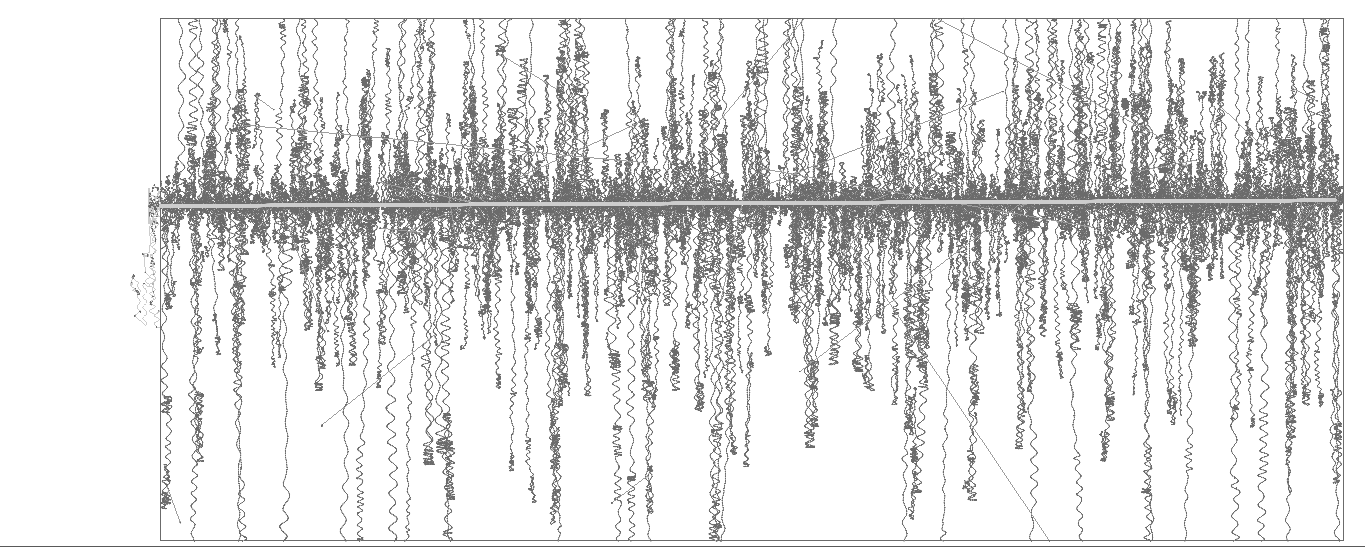
\includegraphics[width=.46\textwidth,valign=c]{deltaE_sideview_neg} \label{fig:deltaE_sideview}}}%

  	 \caption{Geant4 simulation of ${}^{108}$Sn beam at 270 MeV/A in P10 gas. Notice the extent of the delta electrons in the vertical direction as compared to the horizontal extent. }
	\label{fig:deltaE}
\end{figure}


\begin{figure}[!htb]
\includegraphics[width=\textwidth]{padplane_sat.png}
\caption{Results of the algorithm to tag saturated pads, where the black dot denotes a pad was saturated. The charge values plotted is the maximum charge in the pad plane for the entire event.}
\label{fig:satTag}
\end{figure}

Simulating the saturation effects is handled naturally by embedding. Once the time bucket of the saturating signal has been identified, no further signals are embedded since the pad is assumed to be dead. In the case a pad is dead for the whole event, the time of saturation is set to the first time bucket and no signal is embedded for any time bucket. We only need to identify where the time of saturation occurs. The characteristic signature of a saturated signal is the fast fall time of a pulse, which quickly reaches zero, as opposed to the long tail of normal pulses as seen in Figure~\ref{fig:pulseshape}. The long exponential tail can be effectively removed by a software technique which is similar to the electronics concept of pole-zero compensation \cite{polezero}. If the raw ADC value at a particular time, $i$, is represented as $f_i$, the corrected pulse which differentiates out the exponential tail, $f_i^{'}$ can be expressed as, 

\begin{equation}
f_i^{'} = \frac{-b_1\cdot f_{i-1}^{'} + a_o\cdot f_i + a_1 \cdot f_{i-1}}{b_o}
\label{eq:satpolez}
\end{equation}

where $a_o$ = .9723, $a_1$=-.9453, $b_o$=.9545, and $b_1$=-.9203. These coefficients were tuned to remove the long tail of the standard non-saturating pulse, without producing any negative undershoots. If the same procedure is applied to the saturated pulse, the correction produces a negative undershoot, since there was no long exponential tail to begin with. Figure~\ref{fig:pulseshape} shows the pulses as the red curves, and after the pole-zero correction as the blue curves for both the normal and saturated pulses. 

By applying this technique to the real data, we can identify whether a pad has a saturating pulse by looking for this negative undershoot. A negative peak is identified as a saturated signal if it exceeds the threshold of less than -20$\cdot G$ ADC for more than 8 time buckets, and if the max ADC value is > $G\cdot$500, where $G$ is the gain calibration coming from low gain sections discussed in Section~\ref{sec:anodeCalib}. The max ADC condition eliminates false positives which come from  the dead pads where the gating grid subtraction is still applied, introducing large false negative peaks, but have no positive signals. After meeting these two conditions, the pad is flagged as saturated and the time bucket position of saturation is set to $t_{peak} - 5$, where $t_{peak}$ is the time bucket position of the negative peak. This is because the falling edge is around 5 time buckets after the rising edge of the saturation. A separate time is also stored called the MC time bucket position, which sets the point in time in which a signal cannot be embedded any further. This time is set to $t_{peak} - 30$ to ensure that the MC embedded signals do not overlap the real saturating data signal, which would be impossible. These two positions are also shown in Figure~\ref{fig:pulseSatTag}.

There is another way a pad can saturate which occurs when all the pulse heights within the time bucket spectrum add to more than the max ADC threshold of 3500 ADC. This arises since the fall time of the preamplifier circuit is much longer than the time bucket measurement window, and pulses are allowed to pile up in the preamplifier. In this case, no single pulse will reach over the max ADC value yet the last pulse will have a pulse shape that is missing the long characteristic tail, but otherwise looking like a normal pulse. These pulses are also identified by the algorithm described above, since this type of saturated pulse  still has no long tail. 

 When embedding signals into pads, we do not consider the previous amount of total charge in the pad. We assume this type of saturation is a higher order correction, and the current algorithm approximates most of the saturation effects.  Figure~\ref{fig:satTag} shows all of the pads in an event which are tagged by the algorithm as saturated, denoted by the black dots. The max ADC values in a pad are shown in the z-axis color scale, to give a sense of the success of the algorithm. It may appear that the ADC values of some pads appear to be lower than 3500 ADC, but upon further inspection they all satisfy the mode of saturation where the total sum of heights is greater than the max ADC value as mentioned earlier. 

Dead pads are identified earlier in the software when reading in the raw data (STCore class). A dead pad is simply a pad which only contains electronic noise and no signals. A dead pad is identified by having a total ADC r.m.s. value  of less than 50 ADC and a max ADC < 50 over the full time bucket spectrum. Here the dead pad is also tagged as saturated and the time bucket position of saturation is set to the first time bucket. 

%NEED TO ADDRESS WHY THE MAX ADC THRESHOLD IS 3500
%maybe simple pream fig
%maybe example from aki paper about times
%maybe 

%Add figure showing saturated time bucket spectra with location of saturation identified and with pulse shape from embedding I would like to add and how it blocks it.
%Add Figure with 2D pad plane response with and without saturation flag

\subsection{MC and Data Comparison}
\label{sec:mccomparison}
Here we compare several important observables to ensure the MC is simulating the data sufficiently. These observables will be relevant later in the discussion of quality cuts and efficiency analysis discussed in Section~\ref{sec:efficiency}. The most important observable is the total number of clusters, $N_{clust}$. The number of clusters in a track depends on the geometry of the TPC, the spherical angles of the track, and the clustering algorithm. MC tracks were embedded into data for several particle types. The input angular and momentum distribution was uniform. The final measured distributions were weighted such that the angular and momentum distribution matched that of the data for a fair comparison. Figure~\ref{fig:clustcomp} shows the normalized cluster distributions for the MC and data for several particle types. There is no data below $N_{clust} < 20$ because this is the minimum cut to ensure quality PID lines in the data. The normalization is changed for each particle type to display them on the same scale. Very good agreement is seen between the MC and data over a wide range of particle species. 

\begin{figure}[!hbt]
\includegraphics[width=\linewidth]{numcluster.png}
\caption{Comparing the distribution of the number of clusters in MC embedded tracks to experimental data.}
\label{fig:clustcomp}
\end{figure}

The second most important observable is the distance-of-closest-approach (DOCA) to the vertex. Figure~\ref{fig:pocacomp} shows the DOCA distributions for the MC embedded tracks and the data, for the same range of particle species. The distributions were again normalized to different values to display on the same scale. Here the only other cut was the $N_{clust} > 20,$ which cleaned up the background spectrum. It is also worth mentioning the data plotted is also after the space charge correction. Before the space charge correction the distributions would be much wider. It is a fair comparison to compare the space charge corrected data distributions to the MC without space charge effects.  

\begin{figure}[!hbt]
\includegraphics[width=\linewidth]{poca.png}
\caption{Comparison of the DOCA distribution of MC embedded tracks to data.}
\label{fig:pocacomp}
\end{figure}


The other important cut which is made inside of the software is on the PRF distribution of each cluster discussed in Section~\ref{sec:corrTask}. We can also see good agreement between the MC PRF for $\pi^-$ in Figure~\ref{fig:prfpimMC}, and the data PRF, Figure~\ref{fig:prfpimData}, where the black line is the PRF fit to the experimental data. It is sufficient to use such a simple universal PRF function as we can describe all the crossing angle effects discussed in \ref{sec:prf}. Therefore these effects must arise from geometric effects related to the track angle, the amount of charge distributed over an anode wire, and the superposition of the PRF from neighboring anode wires which contribute to the appearance of a changing PRF.

\begin{figure}[!htb]
         \centering
         \includegraphics[width=\textwidth]{PRFs_MC_wcut.png}
         \caption{PRF response of the MC $\pi^-$ tracks.}
         \label{fig:prfpimMC}
\end{figure}


%Add Figure of Pad response function for pion,proton.... for MC vs Data vs angles...
%Add Figure of Number of clusters of MC vs Data
%Add Figure of dEdx MC vs Data
%Add Figure of Momentum resolution MC vs Data
%Add Figure of track residuals? MC vs data?


%\section{Aligning TPC}

%explain the different shifts in the TPC
%BDC shift
%Hit offshet shift




\section{Efficiency Corrections}
\label{sec:efficiency}

Since the \spirit TPC is a fixed target experiment its angular coverage is certainly not 4$\pi$. Because the target is several cm away from the window of the field cage the geometric acceptance is not even 2$\pi$. The rectangular design complicates the calculation of the geometric acceptance of the TPC. Because of this, there are regions of the TPC where it is impossible to reconstruct a track due to the geometric constraints; in these regions the efficiency is exactly 0. In general the efficiency is a function of at least four main parameters. Three define the phase space of a track, momentum $p$ and the two spherical lab angles $\theta_{Lab}$ and $\phi_{Lab}$, and one is the multiplicity of the event. These are the main contributing factors to the efficiency calculations. 

The track efficiency $\epsilon$ is calculated bin-by-bin and is simply written as, 
\begin{equation}
\epsilon = \frac{n_{reco}}{N},
\end{equation}

where $n_{reco}$ is the number of embedded tracks which are successfully reconstructed, and $N$ is the total number of input embedded tracks for that given bin. A track is defined to be successfully reconstructed if it exists in the correlation task described in \ref{sec:embedding}, and therefore meets the minimum criteria for an embedded track, and if it passes the various quality cuts performed on the experimental data set; this could be angular cuts, multiplicity cuts, PID cuts, etc. The TPC's response introduces a finite resolution in both the angles and the momentum. Because of the final measured track could have migrated out of the input bin into another bin. The bin-by-bin correction method is only valid if this effect is small as compared with the size of the bin. If not a more complicated unfolding procedure is needed. A track is defined as successfully reconstructed even it it has migrated out of the bin, and has successfully passed all cuts. The efficiency value is assumed to represent the center of the input MC bin.  
%TALK ABOUT BIN SIZES HEREE????? 

 MC tracks are embedded into a set of \num{e4} on target events and the measured output tracks are correlated to the input track using the embedding software. If the track split in the analysis software, and there are several tracks identified by the software as an embedded track, or part of one, we certainly cannot double count the track as the efficiency is  defined strictly as $\epsilon < 0$. In this case, the track with the minimum distance to vertex is taken for the purposes of calculating efficiency. It is very rare for the later segments of the track to have a distance-to-vertex which originates from the target region. It's reasonable to assume the track with the minimum distance to vertex is the track that best represents the MC input track. The embedded MC tracks are generated as a uniform distribution in $\theta$,$\phi$, and $p$, to ensure each bin has a similar number of input tracks $N$, giving approximately the same statistical error. Here the efficiency distribution is independent of the initial input distribution since we were careful to define reconstructed tracks, as those which may have migrated out of the bin. Neglecting them would make the efficiency biased by the input distribution. Embedding into \num{e4}  events ensures a good sample of the multiplicity distribution, which the efficiency is also a function of. 
 
 \begin{figure}[!htb]%
    \centering
    \subfloat[Polar efficiency plot where $\theta$ is represented by the radius of the circle and $\phi$ is measured as the polar angle made between the y and x axis; this view is  best understood as looking at the TPC from the downstream point of view.]{{\includegraphics[width=.46\textwidth,valign=c]{pim_200_pol.png} \label{fig:pim_pol_eff_ex}}}%
    \qquad
    \subfloat[Cartesian representation of the same efficiency plot  as in the polar plot.]{{\includegraphics[width=.46\textwidth,valign=c]{pim_200_efficiency.png} \label{fig:pim_flat_eff_ex}}}%
	\caption{Efficiency calculations for $\pi^-$ particle traveling at \SI{200}{\mega\eVperc}.}
	\label{fig:pim_eff_ex}
\end{figure}
 
 
Figure~\ref{fig:pim_eff_ex} shows the efficiency calculated for $\pi^-$ tracks traveling with momentum \SI{200}{\mega\eVperc} as a function of the two laboratory angles. It is easiest to visualize the efficiency distribution first in a polar representation which is most like viewing the actual TPC and progressing to a visualization that is better suited to see the values. Figure~\ref{fig:pim_pol_eff_ex} shows the efficiency values plotted in a polar representation where $\theta_{Lab}$ is represented as the radial dimension and $\phi$ is represented as the polar angle. This representation is best understood as if one looked at the tracks in the TPC from the downstream point of view. Of course the vertical direction of the TPC,$\phi$=\ang{90}, is limited in vertical space, therefore tracks are not reconstructed well. The same is the case in downward going tracks, the region centered around $\phi$=\ang{270}. The most efficient regions left and right in the TPC where it has the most acceptance. Though this view is the most intuitive to think about in geometric sense, the values of the efficiency in each bin are difficult to see. Figure~\ref{fig:pim_flat_eff_ex} shows the same efficiency plot but in a Cartesian plot. Here we can see even better the acceptance of downward going tracks, $\phi$=\ang{270}, is greater than the dip in upward going tracks, $\phi$=\ang{90}, resulting from the field cage being shorter in the top than in the bottom, this was due to the space the electronics took up on the top of the TPC, making the field cage asymmetric up and down. 

The area enclosed by the red lines represent the region of the highest efficiency over the full region in $\theta_{Lab}$.  Since we take cuts similar to these in the real data, we assume the efficiency is independent of $\phi$ over these small regions. The efficiency then can be represented as just a function of the two remaining variables. Figure~\ref{fig:132_eff} shows the efficiency of $\pi^-$ and $\pi^+$ particles in the $\tin{132}{124}$ system and Figure~\ref{fig:108_eff} for the $\tin{108}{112}$ system as a function of $\theta_{Lab}$ and momentum $p_{Lab}$. 



\begin{figure}[!htb]%
    \centering
    \subfloat[$\pi^-$ efficiency for $\tin{132}{124}$]{{\includegraphics[width=.46\textwidth,valign=c]{pim_132_efficiency.png} \label{fig:pim_132_eff}}}%
    \qquad
    \subfloat[$\pi^+$ efficiency for $\tin{132}{124}$]{{\includegraphics[width=.46\textwidth,valign=c]{pip_132_efficiency.png} \label{fig:pip_132_eff}}}%
    \caption{Pion efficiencies in the $\tin{132}{124}$ system. }
	\label{fig:132_eff}
\end{figure}



\begin{figure}[!htb]%
    \centering
    \subfloat[$\pi^-$ efficiency for $\tin{108}{112}$]{{\includegraphics[width=.46\textwidth,valign=c]{pim_132_efficiency.png} \label{fig:pim_108_eff}}}%
    \qquad
    \subfloat[$\pi^+$ efficiency for $\tin{108}{112}$]{{\includegraphics[width=.46\textwidth,valign=c]{pip_108_efficiency.png} \label{fig:pip_108_eff}}}%
 	\caption{ Pion efficiencies in the $\tin{108}{112}$ system. }
	\label{fig:108_eff}
\end{figure}



\section{PID Analysis}
\label{sec:pid}
%PID lines over all picture


%PID of pion cut
%background estimation

The energy loss curve in Eq.~\ref{eq:bb} can be described as a 5-parameter general function as, 

\begin{equation}
\frac{dE}{dx} = \frac{p_0}{\beta^{p_3}}(p_1 - \beta^{p_3} + \ln(p_2 + {\beta\gamma}^{-p_4})),
\label{eq:5par_bb}
\end{equation}

where the parameters $p_0-p_4$ are free parameters, $\beta= pc/\sqrt{{pc}^2 + m^2c^4}$, where $m$ is the mass of the particle and $p$ is the momentum. The PID lines vary slightly as a function of the emission angle of each track. The PID was subdivided into 6 pitch angles, $\theta_P = \arctan(p_y/p_z)$, and 6 yaw angles, $\theta_Y = \arctan(p_x/p_z)$, ranging from \ang{-90} to \ang{90} for both. The pion spectra of each yaw-pitch bin was fit with Eq.~\ref{eq:5par_bb} to get the PID line which best describes the data. The distribution around this mean value is not a Gaussian distribution. The variable $z$ has been used before to transform the energy loss of a particular track $dE/dx$ into a more Gaussian variable, defined as

\begin{equation}
z_i = \ln\Big(\frac{\langle dE/dx\rangle}{\langle dE/dx\rangle_i}\Big),
\end{equation}

where $\langle dE/dx\rangle_i$ is the mean energy loss curve fit from Eq.~\ref{eq:5par_bb} for a given particle type $i$. The $z_i$ distribution of the particle of interest will be centered around 0 in this new variable. Figure~\ref{fig:pidpion_raw} shows the typical PID lines zoomed in on the pions. Figure~\ref{fig:pidpion} shows the corresponding $z_i$ distribution after all the pitch-yaw bins have been merged. Both charged pions lie on $z_i=0$, where other particle species rapidly diverge. 


\begin{figure}[!htb]%
    \centering
    \subfloat[Output PID pions.]{{\includegraphics[width=.46\textwidth,valign=c]{pidPion.png} \label{fig:pidpion_raw}}}%
    \qquad
    \subfloat[PID plot for $\pi^-$ and $\pi^+$ species in $z_i$. ]{{\includegraphics[width=.46\textwidth,valign=c]{pidPion_zi.png} \label{fig:pipion_zi}}}%
 	\caption{The charged pion PID plot achieved in the $\tin{132}{124}$ system. PID is achieve by plotting $\langle dE/dx\rangle$ versus particle rigidity, $p/q$. Unique hyperbolic lines show different particle species, where negatively charged particles are plotted as negative rigidity.  }
	\label{fig:pidpion}
\end{figure}


Now that the pion distribution is flattened, we take bin slices along $p/q$ to determine the particle yield in a certain bin and also estimate the background contribution. The background relevant to  the charged pions comes from the $e^+$ and $e^-$ resulting from the $\pi^0$ Dalitz decay described in Appendix~\ref{appen:dalitz}. Figure~\ref{fig:pimmom_flat} shows the Gaussian fits to the $z_i$ distribution for two different $p/q$ binned cuts around the $\pi^-$ particles, whereas Figure~\ref{fig:pipmom_flat} shows the background $\pi^+$ particles. A Gaussian fit is performed to the pions and to the $e$ spectrum to estimate the background contribution. 

\begin{figure}[!htb]%
    \centering
    \subfloat[Bin -54 MeV/c < p/q < -52. ]{{\includegraphics[width=.46\textwidth,valign=c]{pim_mom2.png} \label{fig:pimmom2}}}%
    \qquad
    \subfloat[Bin -68 MeV/c < p/q < -66.]{{\includegraphics[width=.46\textwidth,valign=c]{pim_mom1.png} \label{fig:pimmom1}}}%

    \caption{Flattened PID $z_i$ distribution for binned slices in $p/q$ around the $\pi^-$.}
	\label{fig:pimmom_flat}
\end{figure}


\begin{figure}[!htb]%
    \centering
    \subfloat[Bin 74 MeV/c < p/q < 76.]{{\includegraphics[width=.46\textwidth,valign=c]{pip_mom1.png} \label{fig:pipmom1}}}%
    \qquad
    \subfloat[Bin 94 MeV/c < p/q < 86.]{{\includegraphics[width=.46\textwidth,valign=c]{pip_mom2.png} \label{fig:pipmom2}}}%
 	\caption{Flattened PID $z_i$ distribution  for binned slices in p/q around the $\pi^+$.}
	\label{fig:pipmom_flat}
\end{figure}


We can write the Gaussian fit for the pions as, 

\begin{equation}
G_\pi(z) = A_\pi e^{-\frac{(x-\mu_\pi)^2}{2\sigma_\pi^2}},
\end{equation}

and for the background spectra, in the pion cases $e^+$ and $e^-$:

\begin{equation}
G_B(z) = A_B e^{-\frac{(x-\mu_\pi)^2}{2\sigma_\pi^2} }.
\end{equation}

The probability that a particle is a pion can be described as,

\begin{equation}
P(\pi) = \left( 1 + \frac{A_B}{A_\pi} e^{-\frac{(x-\mu_\pi)^2}{2\sigma_\pi^2}  + \frac{(x-\mu_B)^2}{2\sigma_B^2} } \right)^{-1}
\label{eq:pionProbs}
\end{equation}

The probability value will be used later as a weighting factor when filling the histogram track-by-track as will be discussed in Section~\ref{sec:corrSpectra}. 